% ══════════════════════════════════════════════════════════════════════════════
% Paper A — Archaeometry Submission Wrapper
% Target: Archaeometry (Wiley USG.cls template)
%
% Body content is in manuscript/shared_content.tex (single source of truth).
% This file provides only the Wiley-specific preamble, metadata, and abstract.
%
% SUBMISSION NOTES:
%   - American English spelling used throughout.
%   - Author-date (Harvard) citation system via manual thebibliography.
%   - All LaTeX macros (\NclusterTotal, \simDomePermP, etc.) are generated by:
%       bash manuscript/reproduce_all_macros.sh --macros-only
%   - WORD LIMIT: Archaeometry enforces 8,000 words. Verify before submission.
%   - ABSTRACT: Archaeometry enforces 100-word abstract limit.
%   - KEYWORDS: Maximum 10 keywords.
%   - Zenodo DOI: https://doi.org/10.5281/zenodo.19938283 (v1.6.0, verified)
% ══════════════════════════════════════════════════════════════════════════════

\documentclass[HARVARD,twocolumn]{USG}

% ── Packages ──────────────────────────────────────────────────────────────────
\usepackage[utf8]{inputenc}
\usepackage[T1]{fontenc}
\usepackage{amsmath,amssymb}
\usepackage{booktabs}
\usepackage{graphicx}
\graphicspath{{../figures/}}
\usepackage{array}
\usepackage{microtype}
\usepackage{url}
\usepackage{multirow}
\usepackage{adjustbox}
\setlength{\emergencystretch}{3em}
\newcommand{\degr}{\textdegree{}}

% ── Journal header metadata ────────────────────────────────────────────────────
\articletype{ORIGINAL ARTICLE}
\journal{Archaeometry}
\volume{}
\copyyear{2026}
\startpage{1}

% ══════════════════════════════════════════════════════════════════════════════
%  PIPELINE-GENERATED MACROS
%  All numeric/statistical macros are generated by:
%    bash manuscript/reproduce_all_macros.sh --macros-only
%  Do NOT add \newcommand definitions here — edit the analysis scripts instead.
% ══════════════════════════════════════════════════════════════════════════════
% Generated macros -- 2026-05-08T05:01:40Z
% Source: bash manuscript/reproduce_all_macros.sh
% IMPORTANT: values are computed fresh each run -- do NOT hardcode

% --- analysis/global/emit_constants.py
  \newcommand{\GerizimLon}{35.269}  % anchor longitude, decimal degrees E
  \newcommand{\GerizimLonDMS}{E35~16~08}  % anchor longitude, DMS (from config)
  \newcommand{\GerizimLatDMS}{N32~12~44}  % anchor latitude, DMS (from config)
  \newcommand{\JerusalemLon}{35.232}  % Jerusalem longitude, decimal degrees E
  \newcommand{\GerizimJerusalemSep}{0.037}  % Gerizim-Jerusalem separation (degrees, equatorial)
  \newcommand{\GerizimJerusalemKm}{4.1}  % Gerizim-Jerusalem separation (km, equatorial)
  \newcommand{\NwhcTotal}{1248}  % total UNESCO WHC inscribed sites (all types)
  \newcommand{\NclusterTotalPreCoord}{1013}  % Cultural+Mixed before coordinate filter
  \newcommand{\NexcNatural}{235}  % Natural-only sites excluded from analysis corpus
  \newcommand{\NexcNoCoord}{2}  % Cultural/Mixed sites excluded for missing coordinates
  \newcommand{\NfineSweepSpacings}{7}  % number of spacings in the fine unit sweep (Table tab:unitsweep_fine)
  \newcommand{\NharmonicsCoarse}{120}  % number of 0.1-beru harmonics in 360 degrees
  \newcommand{\simSeed}{42}  % random seed used in all permutation/simulation tests
  \newcommand{\NullRateApp}{4\%}  % geometric null rate for Tier-A++
  \newcommand{\NullRateAp}{10\%}  % geometric null rate for Tier-A+
  \newcommand{\NullRateA}{20\%}  % geometric null rate for Tier-A
  \newcommand{\NullRateB}{100\%}  % geometric null rate for Tier-B
  \newcommand{\NullRateC}{20\%}  % geometric null rate for Tier-C (= A, symmetric)
  \newcommand{\NullRateCMinus}{10\%}  % geometric null rate for Tier-C- (= A+, symmetric)
  \newcommand{\NullRateCMinusTwo}{4\%}  % geometric null rate for Tier-C-- (= A++, symmetric)
  \newcommand{\ApThreshDeg}{0.15}  % A+ threshold (degrees)
  \newcommand{\ApThreshKm}{16.6}  % A+ threshold (km, equatorial)
  \newcommand{\AppThreshDeg}{0.06}  % A++ threshold (degrees)
  \newcommand{\AppThreshKm}{6.66}  % A++ threshold (km, equatorial)
  \newcommand{\ATierThreshDeg}{0.3}  % A-tier threshold (degrees)
  \newcommand{\ATierThreshKm}{33}  % A-tier threshold (km, equatorial)
  \newcommand{\BTierThreshDeg}{1.5}  % B-tier threshold (degrees)
  \newcommand{\BTierThreshKm}{166}  % B-tier threshold (km, equatorial)
  \newcommand{\ApThreshBeru}{0.005}  % A+ threshold (beru) -- appendix use
  \newcommand{\AppThreshBeru}{0.002}  % A++ threshold (beru) -- appendix use
  \newcommand{\ATierThreshBeru}{0.01}  % A-tier threshold (beru) -- appendix use
  \newcommand{\BTierThreshBeru}{0.05}  % B-tier threshold (beru) -- appendix use
  \newcommand{\CMinusThreshDeg}{0.15}  % C- threshold (degrees)
  \newcommand{\CMinusThreshKm}{16.6}  % C- threshold (km)
  \newcommand{\CTierThreshDeg}{0.3}  % C-tier threshold (degrees)
  \newcommand{\CMinusTwoThreshDeg}{0.06}  % C-- threshold (degrees)
  \newcommand{\CMinusThreshBeru}{0.005}  % C- threshold (beru) -- appendix use
  \newcommand{\CTierThreshBeru}{0.01}  % C-tier threshold (beru) -- appendix use
  \newcommand{\CMinusTwoThreshBeru}{0.002}  % C-- threshold (beru) -- appendix use
  \newcommand{\NullRateApPct}{10}  % A+ null rate as plain number (no %)
  \newcommand{\NullRateApFormula}{$2 \times 0.15^\circ / 1.5^\circ$}  % null rate formula in degrees
  \newcommand{\threeStar}{***}  % *** significance shorthand for p<0.001 literal comparisons
  \newcommand{\twoStar}{**}    % ** significance shorthand
  \newcommand{\oneStar}{*}     % * significance shorthand
  \newcommand{\nsLabel}{ns}    % ns label -- use for editorial ns where no single p-value macro exists
  \newcommand{\CorpusPctEurope}{50}  % pct Europe & North America in analysis corpus
  \newcommand{\CorpusPctAsiaPac}{23}  % pct Asia and the Pacific in analysis corpus
  \newcommand{\CorpusPctLatAm}{11}  % pct Latin America & Caribbean in analysis corpus
  \newcommand{\CorpusPctArabStates}{9}  % pct Arab States in analysis corpus
  \newcommand{\CorpusPctAfrica}{7}  % pct Africa in analysis corpus

% --- analysis/global/vonmises_threshold_validation.py
  \newcommand{\vmKappaOwtrad}{9.58}  % von Mises kappa, OWTRAD corpus
  \newcommand{\vmKappaStupa}{6.17}   % von Mises kappa, Q180987 stupa corpus
  \newcommand{\vmKappaRatio}{1.6}  % ratio max/min kappa across corpora
  \newcommand{\vmNOwtrad}{1674}     % N, OWTRAD corpus
  \newcommand{\vmNStupa}{229}      % N, Q180987 stupa corpus
  \newcommand{\vmMixtureWeightOwtrad}{0.0229}  % VM mixture weight, OWTRAD corpus
  \newcommand{\vmMixtureWeightStupa}{0.1297}   % VM mixture weight, stupa corpus
  \newcommand{\vmSigmaBeruOwtrad}{0.00514}   % sigma (beru), OWTRAD -- appendix use
  \newcommand{\vmSigmaBeruStupa}{0.00641}    % sigma (beru), stupa -- appendix use
  \newcommand{\vmSigmaBeruPooled}{0.00529}  % N-weighted pooled sigma (beru) -- appendix use
  \newcommand{\vmSigmaDegOwtrad}{0.1543}   % sigma (degrees), OWTRAD
  \newcommand{\vmSigmaDegStupa}{0.1922}    % sigma (degrees), stupa
  \newcommand{\vmSigmaDegPooled}{0.1588}  % N-weighted pooled sigma (degrees)
  \newcommand{\vmHalfSigmaStupa}{0.0016}  % 0.25*sigma_stupa (beru) -- A++ proxy -- appendix use
  \newcommand{\vmOneSigmaStupa}{0.0032}   % 0.50*sigma_stupa (beru) -- A+  proxy -- appendix use
  \newcommand{\vmTwoSigmaStupa}{0.00641}   % 1.00*sigma_stupa (beru) -- A   proxy -- appendix use
  \newcommand{\vmHalfSigmaDegStupa}{0.048}  % 0.25*sigma_stupa (degrees) -- A++ proxy
  \newcommand{\vmOneSigmaDegStupa}{0.096}   % 0.50*sigma_stupa (degrees) -- A+ proxy
  \newcommand{\vmTwoSigmaDegStupa}{0.1923}   % 1.00*sigma_stupa (degrees) -- A proxy

% --- analysis/global/geodesic_sensitivity.py
  \newcommand{\GeodesicApCurrent}{132}  % A+ count under angular criterion
  \newcommand{\GeodesicApPhysical}{162}  % A+ count under 16.65-km geodesic threshold
  \newcommand{\GeodesicDropOut}{0}  % angular A+ sites that exceed 16.65 km physically
  \newcommand{\GeodesicGainIn}{30}  % non-A+ sites within 16.65 km physically
  \newcommand{\GeodesicThresholdKm}{16.65}  % physical km threshold used in geodesic check
  \newcommand{\GeodesicKmPerDegAtSixty}{55.7}  % east-west km per degree at 60.0degN

% --- analysis/global/owtrad_route_alignment.py
\newcommand{\NOwtradEdges}{1946}
\newcommand{\NOwtradVertices}{1674}
\newcommand{\NOwtradMidApp}{90}
\newcommand{\NOwtradMidAp}{215}
\newcommand{\NOwtradMidA}{420}
\newcommand{\NOwtradVertexApp}{84}
\newcommand{\NOwtradVertexAp}{190}
\newcommand{\NOwtradVertexA}{362}
\newcommand{\NOwtradPerms}{100000}
\newcommand{\NOwtradDegW}{3892}
\newcommand{\NOwtradDegWApp}{211}
\newcommand{\NOwtradDegWAp}{457}
\newcommand{\NOwtradDegWA}{886}
\newcommand{\owtradVertexAppEnrich}{1.25}
\newcommand{\owtradVertexAEnrich}{1.08}
\newcommand{\owtradDegWAppEnrich}{1.36}
\newcommand{\owtradDegWAEnrich}{1.14}
\newcommand{\owtradMidAppEnrich}{1.16}
\newcommand{\owtradMidApEnrich}{1.10}
\newcommand{\owtradMidAEnrich}{1.08}
\newcommand{\zOwtradVertexApp}{2.13}
\newcommand{\zOwtradVertexA}{1.66}
\newcommand{\zOwtradDegWApp}{4.53}
\newcommand{\zOwtradDegWA}{4.31}
\newcommand{\zOwtradMidApp}{1.41}
\newcommand{\zOwtradMidAp}{1.54}
\newcommand{\zOwtradMidA}{1.75}
\newcommand{\pOwtradVertexApp}{0.0224}
\newcommand{\pOwtradVertexAp}{0.0377}
\newcommand{\pOwtradVertexA}{0.0524}
\newcommand{\pOwtradDegWApp}{< 0.0001}
\newcommand{\pOwtradDegWAp}{0.0002}
\newcommand{\pOwtradDegWA}{< 0.0001}
\newcommand{\pOwtradMidApp}{0.0908}
\newcommand{\pOwtradMidAp}{0.0679}
\newcommand{\pOwtradMidAppAdj}{0.3633}
\newcommand{\pOwtradMidApAdj}{0.2715}
\newcommand{\pOwtradMidAppPerm}{0.0799}
\newcommand{\pOwtradMidApPerm}{0.0653}
\newcommand{\pOwtradVertexAppPhase}{0.0202}
\newcommand{\pOwtradVertexApPhase}{0.0491}
\newcommand{\pOwtradMidAppPhase}{0.1006}
\newcommand{\pOwtradMidApPhase}{0.1388}
\newcommand{\NOwtradAppHarmonics}{30}
\newcommand{\NOwtradNonAppHarmonics}{11}
\newcommand{\owtradClustDegRatio}{2.70}
\newcommand{\pOwtradClustDeg}{0.0007}
\newcommand{\pOwtradClustCount}{0.0003}

% --- analysis/global/clustered_control_sweep.py
  \newcommand{\clusterCtrlPermP}{0.522}        % permutation p-value (clustered control sweep)
  \newcommand{\clusterCtrlNsim}{2000}         % number of simulations (clustered control sweep)
  \newcommand{\clusterCtrlTobs}{4.0741}        % observed maximum enrichment ratio
  \newcommand{\clusterCtrlTsimMean}{4.1433}        % mean T_sim across simulations
  \newcommand{\clusterCtrlTsimPctNF}{5.0}        % 95th percentile of T_sim
  \newcommand{\clusterCtrlOmegaMatchPct}{0.0}        % pct of sims where best omega is near 3 deg
  \newcommand{\clusterCtrlPhaseMatchPct}{2.1}        % pct of sims where best phi is near 35 E
  \newcommand{\clusterCtrlObsOmega}{13.75}        % observed best-fit period (deg)
  \newcommand{\clusterCtrlObsPhase}{233.0}        % observed best-fit anchor longitude (deg)
  \newcommand{\clusterCtrlSatTarget}{1.4444}        % saturation target S

% --- analysis/unesco/spherical_monument_test.py
  \newcommand{\pCircApValidated}{0.0076}  % p-value, A+ binomial (context-validated dome corpus)
  \newcommand{\pCircAValidated}{0.0098}   % p-value, A binomial (context-validated dome corpus)
  \newcommand{\circEnrichApValidated}{1.93}  % enrichment ratio, A+ (context-validated dome corpus)
  \newcommand{\NdomeGateNeg}{28}  % number of negative-context gate patterns (Gate 1)
  \newcommand{\NdomeGatePos}{86}  % number of positive-context gate patterns (Gate 2)
  \newcommand{\pCircAppValidatedFisher}{0.0041}  % p-value, A++ Fisher exact dome-validated vs corpus
  \newcommand{\pCircApValidatedFisher}{0.0614}   % p-value, A+ Fisher exact dome-validated vs corpus
  \newcommand{\pCircAValidatedFisher}{0.0346}    % p-value, A Fisher exact dome-validated vs corpus
  \newcommand{\circAppValidatedFisherOR}{3.00}  % OR, A++ Fisher exact dome-validated vs corpus
  \newcommand{\circApValidatedFisherOR}{1.67}   % OR, A+ Fisher exact dome-validated vs corpus
  \newcommand{\circAValidatedFisherOR}{1.64}    % OR, A Fisher exact dome-validated vs corpus
  \newcommand{\NcircValidatedApp}{11}  % Tier-A++ hits (context-validated dome corpus)
  \newcommand{\NcircValidatedAp}{16}   % Tier-A+ hits (context-validated dome corpus)
  \newcommand{\NcircValidatedA}{26}    % Tier-A hits (context-validated dome corpus)

% --- analysis/unesco/spherical_monument_raw_sweep.py
  \newcommand{\NcircTotal}{90}           % raw-sweep population size
  \newcommand{\NcircValidated}{83}             % context-validated population (Test 2)
  \newcommand{\NcircKeywords}{7}               % number of dome-form keywords
  \newcommand{\NcircExcluded}{0}               % excluded (natural/no-coord)
  \newcommand{\NcircContextRejected}{7}               % added by raw sweep vs validated
  \newcommand{\NcircTierApp}{11}           % Tier-A++ hits (raw sweep)
  \newcommand{\NcircTierAp}{18}             % Tier-A+ hits (raw sweep)
  \newcommand{\NcircApRate}{20.0}     % A+ rate (%) = 18/90, rounded to 1 d.p.
  \newcommand{\NcircAppRate}{12.2}     % A++ rate (%) = 11/90, rounded to 1 d.p.
  \newcommand{\NcircTierA}{29}             % Tier-A hits (raw sweep)
  \newcommand{\NcircTierB}{45}             % Tier-B hits (raw sweep)
  \newcommand{\NcircTierC}{9}               % Tier-C hits (raw sweep)
  \newcommand{\pCircApp}{0.0009}         % p-value, A++ binomial (raw sweep)
  \newcommand{\pCircAp}{0.0032}          % p-value, A+ binomial (raw sweep)
  \newcommand{\pCircA}{0.0043}          % p-value, A  binomial (raw sweep)
  \newcommand{\pCircAppFisher}{0.0077}      % p-value, A++ Fisher exact vs rest (raw sweep)
  \newcommand{\circAppFisherOR}{2.71}      % OR, A++ Fisher exact vs rest (raw sweep)
  \newcommand{\pCircApFisher}{0.0346}      % p-value, A+ Fisher exact vs rest (raw sweep)
  \newcommand{\circApFisherOR}{1.77}      % OR, A+ Fisher exact vs rest (raw sweep)
  \newcommand{\pCircAFisher}{0.0175}       % p-value, A Fisher exact vs rest (raw sweep)
  \newcommand{\circAFisherOR}{1.72}       % OR, A Fisher exact vs rest (raw sweep)
  \newcommand{\pCircChi}{0.0732}          % chi-sq uniform, 5 bins, df=4 (raw sweep)
  \newcommand{\GerizimPctileAp}{97}            % anchor-sweep percentile, A+ (raw sweep)
  \newcommand{\GerizimPctileA}{97}            % anchor-sweep percentile, A  (raw sweep)
  \newcommand{\circEnrichAp}{2.00}           % enrichment ratio, A+
  \newcommand{\circEnrichA}{1.61}           % enrichment ratio, A
  \newcommand{\circMeanDev}{0.6586}        % mean deviation in degrees (raw sweep)
  \newcommand{\circEnrichApp}{3.06}           % enrichment ratio, A++
  \newcommand{\circExpAp}{9.0}         % expected A+ count under H0 (= N x 4%)
  \newcommand{\circExpA}{18.0}          % expected A count under H0 (= N x 20%)
  \newcommand{\circARate}{32.2}         % Tier-A rate (%) = 29/90
  \newcommand{\circApCIlo}{12.3}         % Clopper-Pearson 95% CI lower, A+ rate (%)
  \newcommand{\circApCIhi}{29.8}         % Clopper-Pearson 95% CI upper, A+ rate (%)
  \newcommand{\circACIlo}{22.8}          % Clopper-Pearson 95% CI lower, A rate (%)
  \newcommand{\circACIhi}{42.9}          % Clopper-Pearson 95% CI upper, A rate (%)
  \newcommand{\circEnrichCIlo}{1.23}        % Clopper-Pearson 95% CI lower, A+ enrichment ratio
  \newcommand{\circEnrichCIhi}{2.98}        % Clopper-Pearson 95% CI upper, A+ enrichment ratio
  \newcommand{\NcircValidatedApRate}{21.7}  % A+ rate (%) = 18/83, validated pop
  \newcommand{\domeMeanDevDeg}{0.6586}     % mean deviation, dome sites (degrees)
  \newcommand{\domeMeanDevBootP}{0.04364}  % p, bootstrap (Test 2 primary)
  \newcommand{\domeMeanDevDiffKm}{8.51}    % effect size: dome closer by X km
  \newcommand{\fullCorpusMeanDevDeg}{0.7353}  % mean deviation, full corpus (degrees)

% --- analysis/unesco/cluster_asymmetry_test.py
  \newcommand{\clusterRadiusDeg}{0.30}       % cluster radius in degrees (TIER_A_MAX x BERU)
  \newcommand{\NclusterTotal}{1011}          % full Cultural/Mixed corpus
  \newcommand{\NclusterAp}{132}              % Tier-A+ sites
  \newcommand{\clusterApRate}{13.1}           % A+ rate (%)
  \newcommand{\clusterEnrichAp}{1.31}          % enrichment ratio, A+ vs geometric null
  \newcommand{\NclusterExpAp}{101.1}           % expected A+ count under geometric null
  \newcommand{\NclusterExcessAp}{31}          % excess A+ above chance (observed - expected)
  \newcommand{\clusterApBinom}{0.0011}        % binomial p, A+
  \newcommand{\clusterApMean}{6.56}          % mean cluster size, A+ sites
  \newcommand{\clusterNonApMean}{4.96}          % mean cluster size, non-A+ sites
  \newcommand{\clusterRatio}{1.32}           % A+/non-A+ cluster size ratio
  \newcommand{\clusterMWp}{0.0025}        % Mann-Whitney p (site-level)
  \newcommand{\clusterPermP}{0.0000}        % permutation p (site-level)
  \newcommand{\clusterPermZ}{3.96}          % permutation Z-score
  \newcommand{\NpermCluster}{10,000}         % permutation draws, cluster asymmetry test
  \newcommand{\NclusterApHarmonics}{36}              % harmonics with >=1 A+ site
  \newcommand{\NclusterNonApHarmonics}{19}              % harmonics with 0 A+ sites
  \newcommand{\clusterHarmonicApMean}{25.0}          % mean UNESCO sites/harmonic (A+ harmonics)
  \newcommand{\clusterHarmonicNonApMean}{5.9}           % mean UNESCO sites/harmonic (non-A+ harmonics)
  \newcommand{\clusterHarmonicRatio}{4.24}           % harmonic-level density ratio
  \newcommand{\clusterHarmonicMWp}{0.0000}        % Mann-Whitney p (harmonic-level)
  \newcommand{\clusterHarmonicMWpStr}{< 0.0001}  % formatted harmonic MW p-value string
  \newcommand{\NclusterNodeAp}{64}              % node-side A+ sites (phase-split)
  \newcommand{\NclusterAntiAp}{55}              % anti-side A+ sites (phase-split)
  \newcommand{\clusterNodeApMean}{9.25}          % mean cluster size, node-side A+
  \newcommand{\clusterAntiApMean}{6.49}          % mean cluster size, anti-side A+
  \newcommand{\clusterNodeNonApMean}{8.10}          % mean cluster size, node-side non-A+
  \newcommand{\clusterAntiNonApMean}{7.25}          % mean cluster size, anti-side non-A+
  \newcommand{\clusterNodeVsAntiApRatio}{1.43}           % node A+ / anti A+ cluster ratio
  \newcommand{\clusterNodeVsAntiApMWp}{0.0527}        % Mann-Whitney p, node A+ > anti A+
  \newcommand{\clusterNodeAllMean}{8.25}          % mean cluster size, all node-side
  \newcommand{\clusterAntiAllMean}{7.17}          % mean cluster size, all anti-side
  \newcommand{\clusterNodeVsAntiAllMWp}{0.0075}        % Mann-Whitney p, all node > all anti
  \newcommand{\fullMeanDevDeg}{0.7353}      % mean deviation, full corpus (degrees)
  \newcommand{\fullMeanDevPermP}{0.04729}   % p, phase-rotation permutation (Test 1 primary)
  \newcommand{\fullMeanDevZ}{-1.484}       % Z-score, phase-rotation (Test 1)
  \newcommand{\fullMeanDevNullDeg}{0.7500}  % null mean deviation (degrees)
  \newcommand{\spearmanDevClusterRho}{-0.1076}   % Spearman ?, deviation vs cluster size
  \newcommand{\spearmanDevClusterP}{0.00065}  % p, Spearman permutation (Test 3 primary)
  \newcommand{\clusterCondN}{50000}          % perms in conditional subtest
  \newcommand{\clusterCondClusterOk}{6}    % perms reproducing observed clustering
  \newcommand{\clusterCondClusterP}{0.0001}    % p-value, clustering alone (cluster ok / N_COND_PERMS)
  \newcommand{\clusterCondPeakAndCluster}{1}    % perms with clustering AND unit peak
  \newcommand{\clusterCondPeakFrac}{0.1667}    % conditional fraction (peak | cluster)
  \newcommand{\clusterCondPeakFracUncond}{0.1786}    % unconditional peak fraction
  \newcommand{\clusterCondPeakSig}{ns}    % significance label, conditional fraction

% --- analysis/global/emit_cluster_ap_ci.py
  \newcommand{\clusterApCIlo}{11.0}  % Clopper-Pearson 95\% CI lower, A+ rate (%)
  \newcommand{\clusterApCIhi}{15.3}  % Clopper-Pearson 95\% CI upper, A+ rate (%)

% --- analysis/unesco/harmonic_density_attractor_test.py
  \newcommand{\attractorApMeanN}{6.56}           % mean 0.3deg neighbors, A+ sites
  \newcommand{\attractorNonApMeanN}{4.96}           % mean 0.3deg neighbors, non-A+ sites
  \newcommand{\attractorMWp}{0.0025}        % Mann-Whitney p, A+ > non-A+ at 0.3deg
  \newcommand{\attractorMWpWide}{0.1361}        % Mann-Whitney p, A+ > non-A+ at 1.0deg
  \newcommand{\attractorSpearmanRho}{-0.108}          % Spearman rho, dev vs 0.3deg density
  \newcommand{\attractorSpearmanP}{0.00061}       % Spearman p-value
  \newcommand{\attractorHarmonicRatio}{3.83}           % A+ harmonic / non-A+ harmonic density ratio
  \newcommand{\attractorHarmonicMWp}{0.0004}        % Mann-Whitney p, harmonic-level density
  \newcommand{\attractorEUMWp}{0.0005}        % Mann-Whitney p, Europe-only sub-analysis
  \newcommand{\NaraKyotoMaxDist}{34.2}          % max pairwise distance (km), Nara/Kyoto cluster

% --- analysis/unesco/origin_sites_test.py
  \newcommand{\NoriginCorpus}{1011}          % full Cultural/Mixed corpus
  \newcommand{\NoriginAp}{132}              % full-corpus A+ count
  \newcommand{\originApRate}{13.1}            % full-corpus A+ rate (%)
  \newcommand{\pOriginAll}{0.0011}         % p-value, full-corpus A+ binomial
  \newcommand{\originEnrichAll}{1.31}           % enrichment ratio, full corpus
  \newcommand{\NcanonSites}{138}            % sites inscribed 1978-1984 (founding canon)
  \newcommand{\NcanonAp}{19}              % canon A+ count
  \newcommand{\canonApRate}{13.8}            % canon A+ rate (%)
  \newcommand{\pCanon}{0.0950}         % p-value, canon A+ binomial
  \newcommand{\pCanonFisher}{0.4384}    % p-value, canon A+ Fisher exact vs rest
  \newcommand{\orCanonVsRest}{1.07}    % OR, canon A+ Fisher exact vs rest
  \newcommand{\canonEnrich}{1.38}           % enrichment ratio, canon
  \newcommand{\NpreTwoK}{501}            % sites inscribed pre-2000
  \newcommand{\NpreTwoKAp}{66}              % pre-2000 A+ count
  \newcommand{\preTwoKApRate}{13.2}            % pre-2000 A+ rate (%)
  \newcommand{\pPreTwoK}{0.0132}         % p-value, pre-2000 A+ binomial
  \newcommand{\pPreTwoKFisher}{0.4934}   % p-value, pre-2000 A+ Fisher exact vs rest
  \newcommand{\orPreTwoKVsRest}{1.02}   % OR, pre-2000 A+ Fisher exact vs rest
  \newcommand{\preTwoKEnrich}{1.32}           % enrichment ratio, pre-2000
  \newcommand{\NmodernSites}{510}            % sites inscribed 2000+
  \newcommand{\NmodernAp}{66}              % modern A+ count
  \newcommand{\modernApRate}{12.9}            % modern A+ rate (%)
  \newcommand{\pModern}{0.0188}         % p-value, modern A+ binomial
  \newcommand{\modernEnrich}{1.29}           % enrichment ratio, modern
  \newcommand{\pFisherCanonModern}{0.4471}         % Fisher p, canon vs modern
  \newcommand{\orCanonModern}{1.07}           % Fisher OR, canon vs modern
  \newcommand{\NreligUnion}{577}            % any-religion union N
  \newcommand{\NreligUnionAp}{76}              % religion-union A+ count
  \newcommand{\religUnionApRate}{13.2}            % religion-union A+ rate (%)
  \newcommand{\pReligUnion}{0.0085}         % p-value, religion-union A+ binomial
  \newcommand{\pReligUnionFisher}{0.4889}   % p-value, religion-union A+ Fisher exact vs rest
  \newcommand{\pReligChiSq}{0.3136}      % p-value, chi-sq A+ across 5 religion groups
  \newcommand{\religChiSqStat}{4.753}       % chi-sq statistic, religion groups
  \newcommand{\religChiSqDof}{4}                 % df, chi-sq religion groups
  \newcommand{\religUnionFisherOR}{1.02}   % OR, religion-union A+ Fisher exact
  \newcommand{\religUnionEnrich}{1.32}           % enrichment ratio, religion union
  \newcommand{\NchristSites}{397}            % Christian sacred sites N
  \newcommand{\NchristAp}{48}              % Christian sites A+ count
  \newcommand{\christApRate}{12.1}            % Christian sites A+ rate (%)
  \newcommand{\pChrist}{0.0983}         % p-value, Christian sites A+ binomial
  \newcommand{\pChristFisher}{0.7958}      % p-value, Christian A+ Fisher exact vs rest
  \newcommand{\christFisherOR}{0.87}      % OR, Christian A+ Fisher exact
  \newcommand{\NchristA}{93}              % Christian sites A-tier count
  \newcommand{\christARate}{23.4}            % Christian sites A-tier rate (%)
  \newcommand{\pChristA}{0.0522}         % p-value, Christian sites A-tier binomial
  \newcommand{\pChristAFisher}{0.3228}     % p-value, Christian A-tier Fisher exact vs rest
  \newcommand{\christAFisherOR}{1.09}     % OR, Christian A-tier Fisher exact
  \newcommand{\NIslam}{178}            % Islam sacred sites N
  \newcommand{\IslamApCount}{26}              % Islam A+ count
  \newcommand{\IslamApRate}{14.6}            % Islam A+ rate (%)
  \newcommand{\pIslam}{0.0321}         % p-value, Islam A+ binomial
  \newcommand{\pIslamFisher}{0.2853}        % p-value, Islam A+ Fisher exact vs rest
  \newcommand{\islamFisherOR}{1.17}        % OR, Islam A+ Fisher exact
  \newcommand{\NbudSitesRelig}{71}            % Buddhism religion-tagged sites N
  \newcommand{\NbudATier}{20}              % Buddhism A-tier count (dev <= 0.010 beru)
  \newcommand{\budATierRate}{28.2}            % Buddhism A-tier rate (%)
  \newcommand{\budApRateRelig}{21.1}            % Buddhism religion-tagged A+ rate (%)
  \newcommand{\pBudRelig}{0.0040}         % p-value, Buddhism religion-tagged A+ binomial
  \newcommand{\pBudFisher}{0.0335}         % p-value, Buddhism A+ Fisher exact vs rest
  \newcommand{\budFisherOR}{1.88}         % OR, Buddhism A+ Fisher exact
  \newcommand{\NbudInterHarmonic}{19}             % Buddhist C-tier sites (dist_mid <= 0.010 beru)
  \newcommand{\budInterHarmonicRate}{26.8}            % Buddhist C-tier rate (%)
  \newcommand{\budInterHarmonicEnrich}{1.33}           % Buddhist C-tier enrichment vs corpus
  \newcommand{\NInterHarmonicCorpus}{203}           % full-corpus C-tier count
  \newcommand{\corpusInterHarmonicRate}{20.1}           % full-corpus C-tier rate (%)
  \newcommand{\pBudJoint}{0.0052}         % joint p: Buddhism A >= 20 AND C-tier >= 19 (multivariate hypergeometric)
  \newcommand{\NhinSites}{39}            % Hinduism-tagged sites N
  \newcommand{\NhinATier}{11}             % Hinduism A-tier count
  \newcommand{\hinATierRate}{28.2}       % Hinduism A-tier rate (%)
  \newcommand{\hinApCount}{7}               % Hinduism A+ count
  \newcommand{\hinApRate}{17.9}            % Hinduism A+ rate (%)
  \newcommand{\NhinInterHarmonic}{10}             % Hinduism C-tier sites
  \newcommand{\hinInterHarmonicRate}{25.6}            % Hinduism C-tier rate (%)
  \newcommand{\pHinJoint}{0.0324}         % joint p: Hinduism A >= 11 AND C-tier >= 10 (multivariate hypergeometric)
  \newcommand{\NhinCminus}{7}            % Hinduism C- tier sites
  \newcommand{\hinCminusRate}{17.9}            % Hinduism C- tier rate (%)
  \newcommand{\hinCminusEnrich}{1.74}           % Hinduism C- tier enrichment vs corpus
  \newcommand{\pHinCminus}{0.0894}         % p-value, Hinduism C- tier binomial
  \newcommand{\pHinApCminus}{0.0020}         % joint p: Hinduism A+ >= 7 AND C- >= 7 (multivariate hypergeometric)
  \newcommand{\NBudHinShared}{14}            % Buddhism-Hinduism co-tagged sites
  \newcommand{\pBudExclJoint}{0.0123}         % joint p: Buddhism exclusive of shared Hindu sites
  \newcommand{\pHinExclJoint}{0.0862}         % joint p: Hinduism exclusive of shared Buddhist sites

% --- analysis/unesco/founding_sites_analysis.py
  \newcommand{\NthematicTotal}{132}                 % total A+ sites
  \newcommand{\NthematicFounding}{42}             % A+ with founding/origin theme
  \newcommand{\thematicFoundingPct}{32}          % % of A+ with founding theme
  \newcommand{\NthematicCapital}{22}             % founding/capital theme count
  \newcommand{\NthematicMonument}{8}             % monument theme count
  \newcommand{\NthematicSacred}{8}              % sacred/religious theme count
  \newcommand{\NthematicAxis}{4}              % cosmic axis theme count
  \newcommand{\NthematicLandscape}{10}           % sacred landscape theme count
  \newcommand{\NthematicUnclassified}{80}         % unclassified A+ sites
  \newcommand{\NfoundKwAll}{290}                % corpus sites with founding keyword
  \newcommand{\foundKwBaseRate}{28.7}          % base rate, founding keyword (%)
  \newcommand{\NfoundKwAp}{42}             % A+ sites with founding keyword
  \newcommand{\foundKwApRate}{31.8}          % founding keyword rate in A+ (%)
  \newcommand{\NfoundKwNonAp}{248}           % non-A+ sites with founding keyword
  \newcommand{\foundKwNonApRate}{28.2}        % founding keyword rate in non-A+ (%)
  \newcommand{\foundKwFisherOR}{1.19}          % Fisher OR, A+ vs non-A+ founding keyword
  \newcommand{\pFoundKwFisher}{0.225}         % p-value, Fisher test founding keyword
  \newcommand{\NfoundKwApp}{24}              % A++ sites with founding keyword
  \newcommand{\NfoundKwTotalApp}{56}           % total A++ sites
  \newcommand{\foundKwAppRate}{42.9}          % founding keyword rate in A++ (%)
  \newcommand{\foundKwAppFisherOR}{1.94}       % Fisher OR, A++ vs non-A++ founding keyword
  \newcommand{\pFoundKwAppFisher}{0.014}    % p-value, Fisher test founding keyword A++

% --- analysis/unesco/sacred_origin_test.py
  \newcommand{\sacredHitOne}{Lumbini, the Birthplace of the Lord Buddha}  % top-ranked sacred-origin A+ site (by beru deviation)
  \newcommand{\sacredHitTwo}{Historic Centre of Oaxaca and Archaeological Site of Monte Albán}  % 2nd-ranked sacred-origin A+ site
  \newcommand{\sacredHitThree}{Old City of Jerusalem and its Walls}  % 3rd-ranked sacred-origin A+ site

% --- analysis/unesco/meta_keyword_test.py
  \newcommand{\NmetaKeywords}{1741}          % total keyword permutations tested
  \newcommand{\NmetaBeatingChi}{41}           % keywords beating Gerizim chi-sq
  \newcommand{\metaBeatingChiPct}{2.4}         % % of keywords beating Gerizim chi-sq

% --- analysis/unesco/keyword_sensitivity_stupa.py
\newcommand{\kwSensCombinedAN}{26}
\newcommand{\kwSensCombinedAOR}{1.83}
\newcommand{\kwSensCombinedAP}{0.0130}
\newcommand{\kwSensCombinedARate}{31.3}
\newcommand{\kwSensCombinedApN}{16}
\newcommand{\kwSensCombinedApOR}{2.15}
\newcommand{\kwSensCombinedApP}{0.0109}
\newcommand{\kwSensCombinedApRate}{19.3}
\newcommand{\kwSensCombinedAppN}{11}
\newcommand{\kwSensCombinedAppOR}{3.71}
\newcommand{\kwSensCombinedAppP}{< 0.001}
\newcommand{\kwSensCombinedAppRate}{13.3}
\newcommand{\kwSensCombinedN}{83}
\newcommand{\kwSensDomeAN}{19}
\newcommand{\kwSensDomeAOR}{1.65}
\newcommand{\kwSensDomeAP}{0.0554}
\newcommand{\kwSensDomeARate}{29.2}
\newcommand{\kwSensDomeApN}{10}
\newcommand{\kwSensDomeApOR}{1.64}
\newcommand{\kwSensDomeApP}{0.1223}
\newcommand{\kwSensDomeApRate}{15.4}
\newcommand{\kwSensDomeAppN}{7}
\newcommand{\kwSensDomeAppOR}{2.93}
\newcommand{\kwSensDomeAppP}{0.0193}
\newcommand{\kwSensDomeAppRate}{10.8}
\newcommand{\kwSensDomeN}{65}
\newcommand{\kwSensMoundAN}{0}
\newcommand{\kwSensMoundApN}{0}
\newcommand{\kwSensMoundAppN}{0}
\newcommand{\kwSensMoundN}{0}
\newcommand{\kwSensNoStupaAN}{19}
\newcommand{\kwSensNoStupaAOR}{1.65}
\newcommand{\kwSensNoStupaAP}{0.0554}
\newcommand{\kwSensNoStupaARate}{29.2}
\newcommand{\kwSensNoStupaApN}{10}
\newcommand{\kwSensNoStupaApOR}{1.64}
\newcommand{\kwSensNoStupaApP}{0.1223}
\newcommand{\kwSensNoStupaApRate}{15.4}
\newcommand{\kwSensNoStupaAppN}{7}
\newcommand{\kwSensNoStupaAppOR}{2.93}
\newcommand{\kwSensNoStupaAppP}{0.0193}
\newcommand{\kwSensNoStupaAppRate}{10.8}
\newcommand{\kwSensNoStupaN}{65}
\newcommand{\kwSensStupaAN}{7}
\newcommand{\kwSensStupaAOR}{2.55}
\newcommand{\kwSensStupaAP}{0.0536}
\newcommand{\kwSensStupaARate}{38.9}
\newcommand{\kwSensStupaApN}{6}
\newcommand{\kwSensStupaApOR}{4.5}
\newcommand{\kwSensStupaApP}{0.0072}
\newcommand{\kwSensStupaApRate}{33.3}
\newcommand{\kwSensStupaAppN}{4}
\newcommand{\kwSensStupaAppOR}{6.94}
\newcommand{\kwSensStupaAppP}{0.0057}
\newcommand{\kwSensStupaAppRate}{22.2}
\newcommand{\kwSensStupaN}{18}

% --- analysis/unesco/temporal_gradient_test.py
  \newcommand{\ZcochranThree}{-0.206}       % Cochran-Armitage Z, A+, 3-bin
  \newcommand{\pCochranThree}{0.4184}      % p-value, Cochran-Armitage A+, 3-bin
  \newcommand{\ZcochranFive}{0.190}         % Cochran-Armitage Z, A+, 5-bin
  \newcommand{\pCochranFive}{0.5752}      % p-value, Cochran-Armitage A+, 5-bin
  \newcommand{\ZcochranAppThree}{-1.664}  % Cochran-Armitage Z, A++, 3-bin
  \newcommand{\pCochranAppThree}{0.0481} % p-value, Cochran-Armitage A++, 3-bin
  \newcommand{\ZcochranAppFive}{-1.655}   % Cochran-Armitage Z, A++, 5-bin
  \newcommand{\pCochranAppFive}{0.0489}  % p-value, Cochran-Armitage A++, 5-bin
  \newcommand{\pCanonApp}{0.0232}       % p-value, A++ binomial, canon cohort (1978-1984)
  \newcommand{\canonAppRate}{8.0}     % A++ rate (%), canon cohort
  \newcommand{\NcohortAppA}{138}         % N, A++ canon cohort
  \newcommand{\NcohortAppAapp}{11}   % A++ count, canon cohort
  \newcommand{\cohortAppArate}{8.0}   % A++ rate (%), canon cohort (alias)
  \newcommand{\cohortAppErate}{4.5}  % A++ rate (%), modern cohort (2000-2025)
  \newcommand{\rhoSpearman}{0.0146}        % Spearman rho, A+ rate vs era
  \newcommand{\pSpearman}{0.643431}        % p-value, Spearman rank correlation
  \newcommand{\NcohortRawA}{138}  % 1978-1984 cohort N
  \newcommand{\NcohortRawAap}{19}  % 1978-1984 cohort A+ count
  \newcommand{\cohortRawArate}{13.8}  % 1978-1984 cohort A+ rate (%)
  \newcommand{\NcohortA}{138}  % 1978-1984 cohort N (alias)
  \newcommand{\NcohortAap}{19}  % 1978-1984 cohort A+ count (alias)
  \newcommand{\cohortArate}{13.8}  % 1978-1984 cohort A+ rate (%) (alias)
  \newcommand{\NcohortRawB}{141}  % 1985-1991 cohort N
  \newcommand{\NcohortRawBap}{14}  % 1985-1991 cohort A+ count
  \newcommand{\cohortRawBrate}{9.9}  % 1985-1991 cohort A+ rate (%)
  \newcommand{\NcohortB}{141}  % 1985-1991 cohort N (alias)
  \newcommand{\NcohortBap}{14}  % 1985-1991 cohort A+ count (alias)
  \newcommand{\cohortBrate}{9.9}  % 1985-1991 cohort A+ rate (%) (alias)
  \newcommand{\NcohortRawC}{222}  % 1992-1999 cohort N
  \newcommand{\NcohortRawCap}{33}  % 1992-1999 cohort A+ count
  \newcommand{\cohortRawCrate}{14.9}  % 1992-1999 cohort A+ rate (%)
  \newcommand{\NcohortC}{222}  % 1992-1999 cohort N (alias)
  \newcommand{\NcohortCap}{33}  % 1992-1999 cohort A+ count (alias)
  \newcommand{\cohortCrate}{14.9}  % 1992-1999 cohort A+ rate (%) (alias)
  \newcommand{\NcohortRawD}{211}  % 2000-2009 cohort N
  \newcommand{\NcohortRawDap}{26}  % 2000-2009 cohort A+ count
  \newcommand{\cohortRawDrate}{12.3}  % 2000-2009 cohort A+ rate (%)
  \newcommand{\NcohortD}{211}  % 2000-2009 cohort N (alias)
  \newcommand{\NcohortDap}{26}  % 2000-2009 cohort A+ count (alias)
  \newcommand{\cohortDrate}{12.3}  % 2000-2009 cohort A+ rate (%) (alias)
  \newcommand{\NcohortRawE}{299}  % 2010-2025 cohort N
  \newcommand{\NcohortRawEap}{40}  % 2010-2025 cohort A+ count
  \newcommand{\cohortRawErate}{13.4}  % 2010-2025 cohort A+ rate (%)
  \newcommand{\NcohortE}{299}  % 2010-2025 cohort N (alias)
  \newcommand{\NcohortEap}{40}  % 2010-2025 cohort A+ count (alias)
  \newcommand{\cohortErate}{13.4}  % 2010-2025 cohort A+ rate (%) (alias)
  \newcommand{\pAdjTestTwoB}{---}  % Test 2b excluded from Bonferroni (sensitivity variant, not independent)

% --- analysis/unesco/deep_temporal_analysis.py
  \newcommand{\NdatedSites}{579}          % sites with known founding date
  \newcommand{\NpreCE}{173}             % pre-CE (antiquity) sites
  \newcommand{\NpreCEap}{22}            % A+ sites pre-CE
  \newcommand{\preCErate}{12.7}           % A+ rate in pre-CE sites (%)
  \newcommand{\preCEenrich}{1.27}          % enrichment, pre-CE A+
  \newcommand{\pPreCEbinom}{0.1441}        % p-value, pre-CE A+ binomial
  \newcommand{\NpostCE}{406}            % post-CE sites
  \newcommand{\NpostCEap}{51}           % A+ sites post-CE
  \newcommand{\postCErate}{12.6}           % A+ rate in post-CE sites (%)
  \newcommand{\preCEfisherOR}{1.01}          % Fisher OR, pre- vs post-CE A+
  \newcommand{\pPreCEfisher}{0.5285}         % p-value, Fisher pre- vs post-CE
  \newcommand{\NapPreCE}{22}           % A+ sites with pre-CE founding date
  \newcommand{\apPreCEpct}{17}            % % of all A+ that are pre-CE
  \newcommand{\NapDeep}{8}             % A+ sites deeply pre-CE (antiquity)
  \newcommand{\apPreCEofDated}{30}           % % of dated A+ that are pre-CE
  \newcommand{\nonApPreCEpct}{30}           % % of dated non-A+ that are pre-CE
  \newcommand{\preCEantiqFisherOR}{1.01}       % Fisher OR, A+ vs non-A+ pre-CE antiquity
  \newcommand{\pPreCEantiqFisher}{0.0226}         % p-value, A+ vs non-A+ antiquity Fisher
  \newcommand{\rhoFoundDate}{0.0117}          % Spearman rho, founding date vs A+ status
  \newcommand{\pFoundDateSpearman}{0.7796}      % p-value, founding date Spearman
  \newcommand{\earlyModernN}{126}  % early modern (1500-1800 CE) N
  \newcommand{\earlyModernAp}{18}  % early modern A+ count
  \newcommand{\earlyModernRate}{14.3}  % early modern A+ rate (%)
  \newcommand{\pEarlyModern}{0.0778}  % p-value, early modern binomial
  \newcommand{\canonPostCEN}{53}  % canon (<=1984) sites with post-CE founding date N
  \newcommand{\canonPostCEap}{9}  % canon + post-CE A+ count
  \newcommand{\canonPostCErate}{17.0}  % canon + post-CE A+ rate (%)
  \newcommand{\pCanonPostCE}{0.0785}  % p-value, canon + post-CE binomial
  \newcommand{\peakSigYear}{2024}             % UNESCO inscription year with peak A+ signal
  \newcommand{\peakSigN}{989}              % cumulative sites at peak signal year
  \newcommand{\peakSigAp}{131}             % cumulative A+ at peak signal year
  \newcommand{\peakSigRate}{13.2}           % A+ rate at peak signal year (%)
  \newcommand{\peakSigP}{0.00063459}     % p-value at peak signal year
  \newcommand{\peakNegLogP}{3.20}          % -log10(p) at peak signal year
  \newcommand{\firstSigYear}{1997}           % first year A+ signal reached p<0.05
  \newcommand{\firstSigN}{438}             % cumulative sites at first significant year
  \newcommand{\firstSigRate}{12.8}          % A+ rate at first significance (%)
  \newcommand{\NfirstHalf}{505}             % sites inscribed in first half of UNESCO record
  \newcommand{\NapFirstHalf}{67}            % A+ sites in first half
  \newcommand{\firstHalfRate}{13.3}           % A+ rate in first half (%)
  \newcommand{\pFirstHalf}{0.010907}       % p-value, first-half A+ binomial
  \newcommand{\NsecondHalf}{506}            % sites inscribed in second half of UNESCO record
  \newcommand{\NapSecondHalf}{65}           % A+ sites in second half
  \newcommand{\secondHalfRate}{12.8}           % A+ rate in second half (%)
  \newcommand{\pSecondHalf}{0.022568}       % p-value, second-half A+ binomial
  \newcommand{\halfFisherOR}{1.04}          % Fisher OR, first vs second half A+
  \newcommand{\pHalfFisher}{0.457987}       % p-value, Fisher half-corpus comparison
  \newcommand{\blockOneRate}{14.0}  % A+ rate in sites 1-100 (block 1)
  \newcommand{\pBlockOne}{0.1239}  % binomial p, block 1
  \newcommand{\blockThreeRate}{16.0}  % A+ rate in sites 201-300 (block 3)
  \newcommand{\pBlockThree}{0.0399}  % binomial p, block 3
  \newcommand{\blockFiveRate}{17.0}  % A+ rate in sites 401-500 (block 5)
  \newcommand{\pBlockFive}{0.0206}  % binomial p, block 5

% --- analysis/global/anchor_uniqueness_audit.py
  \newcommand{\anchorSweepNanchors}{36{,}000}          % number of anchor points in sweep
  \newcommand{\anchorSweepApMean}{101.2}           % mean A+ count across all anchors
  \newcommand{\anchorSweepApStd}{10.9}            % std A+ count across all anchors
  \newcommand{\anchorSweepGlobalMax}{133}           % global max A+ at any anchor
  \newcommand{\anchorSweepGlobalMaxA}{133}           % global max A+ (symmetric corpus)
  \newcommand{\optimalPhaseApA}{133}           % max A+ at any x.18degE anchor
  \newcommand{\GerizimSweepApp}{56}             % Gerizim A++ in sweep
  \newcommand{\GerizimSweepAp}{132}              % Gerizim A+ in sweep
  \newcommand{\GerizimSweepA}{228}             % Gerizim A in sweep
  \newcommand{\anchorSweepPctile}{99.7}          % Gerizim percentile in A+ anchor sweep
  \newcommand{\anchorSweepGeApPct}{0.66}          % % of anchors beating Gerizim A+
  \newcommand{\JerusalemSweepApp}{57}           % Jerusalem A++ in sweep
  \newcommand{\JerusalemSweepAp}{128}            % Jerusalem A+ in sweep
  \newcommand{\JerusalemSweepA}{218}           % Jerusalem A in sweep
  \newcommand{\JerusalemSweepPctile}{97.7}        % Jerusalem percentile in A+ anchor sweep
  \newcommand{\anchorSweepJerApPct}{3.00}          % % of anchors beating Jerusalem A+
  \newcommand{\anchorSweepTopPct}{2.3}          % top-N% globally (corridor, both anchors)
  \newcommand{\sweepABDiff}{4}          % A+ count difference Gerizim vs Jerusalem

% --- analysis/unesco/verify_phase_peak_periodicity.py
  \newcommand{\xbandLabel}{x.25}         % optimal phase band label (e.g. x.21degE)
  \newcommand{\optimalPhase}{2.25}          % optimal phase (degrees mod 3)
  \newcommand{\optimalPhaseAp}{132}           % A+ count at optimal phase
  \newcommand{\GerizimPhase}{2.269}         % Gerizim longitude mod 3
  \newcommand{\phaseGap}{0.019}           % gap between Gerizim and optimal phase (deg)
  \newcommand{\phaseGapKm}{1.8}           % phase gap converted to km

% --- analysis/global/peak_geography_audit.py
  \newcommand{\JerichoAnchorAp}{111}           % A+ count with Jericho as anchor
  \newcommand{\DeadSeaAnchorAp}{103}          % A+ count with Dead Sea center as anchor
  \newcommand{\MtNeboAnchorAp}{97}           % A+ count with Mt Nebo as anchor
  \newcommand{\DamascusAnchorAp}{101}          % A+ count with Damascus as anchor
  \newcommand{\localBestLon}{35.242}          % longitude of local peak A+ in Levant sweep
  \newcommand{\localBestAp}{133}           % A+ count at local peak longitude

% --- analysis/global/landmark_anchor_ranking.py
  \newcommand{\GerizimTempleAp}{132}          % A+ count at Gerizim Temple anchor
  \newcommand{\GerizimTempleRank}{8}          % rank of Gerizim Temple among all landmarks

% --- analysis/global/anchor_site_comparison.py
  \newcommand{\LumbiniDevKm}{0.79}          % Lumbini deviation from Gerizim (km)
  \newcommand{\LumbiniDevM}{789}           % Lumbini deviation from Gerizim (m)
  \newcommand{\LumbiniDevBeru}{0.000237}      % Lumbini deviation from Gerizim (beru)
  \newcommand{\LumbiniTier}{A++}            % Lumbini tier relative to Gerizim
  \newcommand{\LumbiniJerDevKm}{4.93}        % Lumbini deviation from Jerusalem (km)
  \newcommand{\LumbiniJerDevBeru}{0.001480}    % Lumbini deviation from Jerusalem (beru)
  \newcommand{\LumbiniJerTier}{A++}          % Lumbini tier relative to Jerusalem
  \newcommand{\TakhtGerizimDevKm}{3.77}       % Takht-e Soleyman deviation from Gerizim (km)
  \newcommand{\TakhtGerizimDevBeru}{0.001133}   % Takht-e Soleyman deviation from Gerizim (beru)
  \newcommand{\TakhtGerizimTier}{A++}         % Takht-e Soleyman tier relative to Gerizim
  \newcommand{\TakhtJerDevKm}{0.37}          % Takht-e Soleyman deviation from Jerusalem (km)
  \newcommand{\TakhtJerDevM}{366}         % Takht-e Soleyman deviation from Jerusalem (m)
  \newcommand{\TakhtJerDevBeru}{0.000110}      % Takht-e Soleyman deviation from Jerusalem (beru)
  \newcommand{\TakhtJerTier}{A++}            % Takht-e Soleyman tier relative to Jerusalem
  \newcommand{\KhojaGerizimDevKm}{0.23}       % Khoja Ahmed Yasawi deviation from Gerizim (km)
  \newcommand{\KhojaGerizimDevBeru}{0.000069}   % Khoja Ahmed Yasawi deviation from Gerizim (beru)
  \newcommand{\KhojaGerizimTier}{A++}         % Khoja Ahmed Yasawi tier relative to Gerizim
  \newcommand{\KhojaJerDevKm}{4.37}          % Khoja Ahmed Yasawi deviation from Jerusalem (km)
  \newcommand{\KhojaJerDevBeru}{0.001312}      % Khoja Ahmed Yasawi deviation from Jerusalem (beru)
  \newcommand{\KhojaJerTier}{A++}            % Khoja Ahmed Yasawi tier relative to Jerusalem
  \newcommand{\NappTotal}{56}             % total A++ sites from Gerizim anchor
  \newcommand{\GerizimAppCount}{56}        % Gerizim A++ count (alias)
  \newcommand{\WPPDeltaKm}{0.59}          % World Peace Pagoda deviation from Gerizim (km)
  \newcommand{\WPPDeltaBeru}{0.000177}      % World Peace Pagoda deviation from Gerizim (beru)
  \newcommand{\topHitNameOne}{\textit{Sacri Monti} of Piedmont and Lombardy}  % rank-one A++ site name
  \newcommand{\topHitLonOne}{8.2697}  % rank-one A++ site longitude (degE)
  \newcommand{\topHitDevBeruOne}{0.000024}  % rank-one beru deviation
  \newcommand{\topHitDevKmOne}{0.08}  % rank-one deviation (km)
  \newcommand{\topHitDevMOne}{80}  % rank-one deviation (m)
  \newcommand{\topHitOne}{Sacri Monti}  % rank-one short name
  \newcommand{\appSiteNameOne}{\textit{Sacri Monti} of Piedmont and Lombardy}  % A++ table rank One: name
  \newcommand{\appSiteLonOne}{8.2697}  % A++ table rank One: longitude
  \newcommand{\appSiteDevBeruOne}{0.000024}  % A++ table rank One: beru deviation
  \newcommand{\appSiteDevKmOne}{0.08}  % A++ table rank One: km
  \newcommand{\appSiteDevMOne}{80}  % A++ table rank One: m
  \newcommand{\topHitNameTwo}{Mausoleum of Khoja Ahmed Yasawi}  % rank-two A++ site name
  \newcommand{\topHitLonTwo}{68.2711}  % rank-two A++ site longitude (degE)
  \newcommand{\topHitDevBeruTwo}{0.000069}  % rank-two beru deviation
  \newcommand{\topHitDevKmTwo}{0.23}  % rank-two deviation (km)
  \newcommand{\topHitDevMTwo}{228}  % rank-two deviation (m)
  \newcommand{\topHitTwo}{Khoja Ahmed Yasawi}  % rank-two short name
  \newcommand{\appSiteNameTwo}{Mausoleum of Khoja Ahmed Yasawi}  % A++ table rank Two: name
  \newcommand{\appSiteLonTwo}{68.2711}  % A++ table rank Two: longitude
  \newcommand{\appSiteDevBeruTwo}{0.000069}  % A++ table rank Two: beru deviation
  \newcommand{\appSiteDevKmTwo}{0.23}  % A++ table rank Two: km
  \newcommand{\appSiteDevMTwo}{228}  % A++ table rank Two: m
  \newcommand{\topHitNameThree}{Site of Palmyra}  % rank-three A++ site name
  \newcommand{\topHitLonThree}{38.2667}  % rank-three A++ site longitude (degE)
  \newcommand{\topHitDevBeruThree}{0.000078}  % rank-three beru deviation
  \newcommand{\topHitDevKmThree}{0.26}  % rank-three deviation (km)
  \newcommand{\topHitDevMThree}{259}  % rank-three deviation (m)
  \newcommand{\topHitThree}{Site of Palmyra}  % rank-three short name
  \newcommand{\appSiteNameThree}{Site of Palmyra}  % A++ table rank Three: name
  \newcommand{\appSiteLonThree}{38.2667}  % A++ table rank Three: longitude
  \newcommand{\appSiteDevBeruThree}{0.000078}  % A++ table rank Three: beru deviation
  \newcommand{\appSiteDevKmThree}{0.26}  % A++ table rank Three: km
  \newcommand{\appSiteDevMThree}{259}  % A++ table rank Three: m
  \newcommand{\appSiteNameFour}{Boyana Church}  % A++ table rank Four: name
  \newcommand{\appSiteLonFour}{23.2662}  % A++ table rank Four: longitude
  \newcommand{\appSiteDevBeruFour}{0.000094}  % A++ table rank Four: beru deviation
  \newcommand{\appSiteDevKmFour}{0.31}  % A++ table rank Four: km
  \newcommand{\appSiteDevMFour}{312}  % A++ table rank Four: m
  \newcommand{\appSiteNameFive}{Antigua Guatemala}  % A++ table rank Five: name
  \newcommand{\appSiteLonFive}{-90.7282}  % A++ table rank Five: longitude
  \newcommand{\appSiteDevBeruFive}{0.000095}  % A++ table rank Five: beru deviation
  \newcommand{\appSiteDevKmFive}{0.32}  % A++ table rank Five: km
  \newcommand{\appSiteDevMFive}{315}  % A++ table rank Five: m
  \newcommand{\appSiteNameSix}{Hola\v{s}ovice Historic Village}  % A++ table rank Six: name
  \newcommand{\appSiteLonSix}{14.2726}  % A++ table rank Six: longitude
  \newcommand{\appSiteDevBeruSix}{0.000120}  % A++ table rank Six: beru deviation
  \newcommand{\appSiteDevKmSix}{0.40}  % A++ table rank Six: km
  \newcommand{\appSiteDevMSix}{401}  % A++ table rank Six: m
  \newcommand{\appSiteNameSeven}{Historic Town of Grand-Bassam}  % A++ table rank Seven: name
  \newcommand{\appSiteLonSeven}{-3.7364}  % A++ table rank Seven: longitude
  \newcommand{\appSiteDevBeruSeven}{0.000180}  % A++ table rank Seven: beru deviation
  \newcommand{\appSiteDevKmSeven}{0.60}  % A++ table rank Seven: km
  \newcommand{\appSiteDevMSeven}{598}  % A++ table rank Seven: m
  \newcommand{\appSiteNameEight}{Lumbini, the Birthplace of the Lord Buddha}  % A++ table rank Eight: name
  \newcommand{\appSiteLonEight}{83.2761}  % A++ table rank Eight: longitude
  \newcommand{\appSiteDevBeruEight}{0.000237}  % A++ table rank Eight: beru deviation
  \newcommand{\appSiteDevKmEight}{0.79}  % A++ table rank Eight: km
  \newcommand{\appSiteDevMEight}{789}  % A++ table rank Eight: m
  \newcommand{\appSiteNameNine}{Br\^{a}ncu\c{s}i Monumental Ensemble of T\^{a}rgu Jiu}  % A++ table rank Nine: name
  \newcommand{\appSiteLonNine}{23.2788}  % A++ table rank Nine: longitude
  \newcommand{\appSiteDevBeruNine}{0.000326}  % A++ table rank Nine: beru deviation
  \newcommand{\appSiteDevKmNine}{1.09}  % A++ table rank Nine: km
  \newcommand{\appSiteDevMNine}{1085}  % A++ table rank Nine: m
  \newcommand{\appSiteNameTen}{Historic Centre of Florence}  % A++ table rank Ten: name
  \newcommand{\appSiteLonTen}{11.2561}  % A++ table rank Ten: longitude
  \newcommand{\appSiteDevBeruTen}{0.000430}  % A++ table rank Ten: beru deviation
  \newcommand{\appSiteDevKmTen}{1.43}  % A++ table rank Ten: km
  \newcommand{\appSiteDevMTen}{1431}  % A++ table rank Ten: m
  \newcommand{\JerusalemAp}{127}  % Jerusalem A+ count (self-excluded corpus)
  \newcommand{\NjerSelfExclCorpus}{1010}  % corpus size, Jerusalem self-excluded (Sweep B)
  \newcommand{\NgerizimSweepCorpus}{1011}  % corpus size for sweep focal anchors (extended 1012, self-exclusion -1)
  \newcommand{\pJerusalemAp}{0.0047}  % p-value, Jerusalem A+ binomial (self-excluded)
  \newcommand{\MeccaAp}{107}  % Mecca A+ count (full corpus)
  \newcommand{\pMeccaAnchor}{0.2825}  % p-value, Mecca binomial (A+, one-sided)
  \newcommand{\MeruAp}{104}  % Mt. Meru (Tanzania, 36.750E) A+ count
  \newcommand{\pMeruAnchor}{0.3956}  % p-value, Mt. Meru binomial (A+, one-sided)
  \newcommand{\KailashAp}{104}  % Mt. Kailash (81.312E) A+ count
  \newcommand{\pKailashAnchor}{0.3956}  % p-value, Kailash binomial (A+, one-sided)

% --- analysis/unesco/spatial_independence_test.py
  \newcommand{\DEFFhalf}{1.842}          % design effect (DEFF), half-degree blocks
  \newcommand{\NeffHalf}{549}            % effective N, half-degree blocks
  \newcommand{\pNeffHalf}{0.011}           % p-value, A+ test with effective N (half-deg)
  \newcommand{\ICChalf}{0.187}           % intracluster correlation, half-degree blocks
  \newcommand{\DEFFquarter}{1.974}         % design effect (DEFF), quarter-degree blocks
  \newcommand{\NeffQuarter}{512}          % effective N, quarter-degree blocks
  \newcommand{\pNeffQuarter}{0.014}         % p-value, A+ test with effective N (quarter-deg)
  \newcommand{\blockBootCIlo}{10.50}        % block-bootstrap CI lower bound, A+ rate (%)
  \newcommand{\blockBootCIhi}{15.43}        % block-bootstrap CI upper bound, A+ rate (%)
  \newcommand{\blockBootZ}{2.42}           % block-bootstrap Z-score, A+

% --- analysis/unesco/regional_temporal_gradient.py
  \newcommand{\pLogRegCohort}{0.7206}   % logistic regression cohort p
  \newcommand{\orLogRegCohort}{0.954}  % logistic regression cohort OR per step
  \newcommand{\zLogRegCohort}{-0.358}   % logistic regression cohort Z
  \newcommand{\pLogRegCohortApp}{0.0784}   % logistic regression cohort p (A++)
  \newcommand{\orLogRegCohortApp}{0.722}  % logistic regression cohort OR per step (A++)
  \newcommand{\zLogRegCohortApp}{-1.760}   % logistic regression cohort Z (A++)
  \newcommand{\MHcommonOR}{1.065}             % MH common OR (early vs late)
  \newcommand{\CMHchisq}{0.109}              % CMH chi-squared
  \newcommand{\pCMH}{0.7418}                  % CMH p-value
  \newcommand{\stratNconcordant}{3}    % regions with early > late
  \newcommand{\stratNregions}{5}   % total regions tested
  \newcommand{\stratNsig}{0}          % regions sig at p<0.05
  \newcommand{\stratVerdict}{directionally consistent but underpowered within strata}
  \newcommand{\pRegionEmpAll}{0.7978}    % region-specific empirical null, all sites
  \newcommand{\pRegionEmpPreTwoK}{0.7534}  % region-specific empirical null, pre-2000
  \newcommand{\EuropeNAN}{487}  % N sites, Europe & North America
  \newcommand{\EuropeNAApCount}{62}  % A+ count, Europe & North America
  \newcommand{\EuropeNAApRate}{12.7}  % A+ rate (%), Europe & North America
  \newcommand{\EuropeNAApShare}{47.0}  % share of total A+, Europe & North America
  \newcommand{\EuropeNAEarlyApRate}{13.7}  % early A+ rate (pre-2000), Europe & North America
  \newcommand{\EuropeNALateApRate}{11.6}   % late A+ rate (2000+), Europe & North America
  \newcommand{\AsiaPacN}{232}  % N sites, Asia & Pacific
  \newcommand{\AsiaPacApCount}{34}  % A+ count, Asia & Pacific
  \newcommand{\AsiaPacApRate}{14.7}  % A+ rate (%), Asia & Pacific
  \newcommand{\AsiaPacApShare}{25.8}  % share of total A+, Asia & Pacific
  \newcommand{\AsiaPacEarlyApRate}{15.4}  % early A+ rate (pre-2000), Asia & Pacific
  \newcommand{\AsiaPacLateApRate}{14.2}   % late A+ rate (2000+), Asia & Pacific
  \newcommand{\AfricaN}{68}  % N sites, Africa
  \newcommand{\AfricaApCount}{11}  % A+ count, Africa
  \newcommand{\AfricaApRate}{16.2}  % A+ rate (%), Africa
  \newcommand{\AfricaApShare}{8.3}  % share of total A+, Africa
  \newcommand{\AfricaEarlyApRate}{9.5}  % early A+ rate (pre-2000), Africa
  \newcommand{\AfricaLateApRate}{19.1}   % late A+ rate (2000+), Africa
  \newcommand{\ArabStatesN}{110}  % N sites, Arab States
  \newcommand{\ArabStatesApCount}{15}  % A+ count, Arab States
  \newcommand{\ArabStatesApRate}{13.6}  % A+ rate (%), Arab States
  \newcommand{\ArabStatesApShare}{11.4}  % share of total A+, Arab States
  \newcommand{\ArabStatesEarlyApRate}{10.9}  % early A+ rate (pre-2000), Arab States
  \newcommand{\ArabStatesLateApRate}{16.4}   % late A+ rate (2000+), Arab States
  \newcommand{\LatAmN}{114}  % N sites, Latin America & Caribbean
  \newcommand{\LatAmApCount}{10}  % A+ count, Latin America & Caribbean
  \newcommand{\LatAmApRate}{8.8}  % A+ rate (%), Latin America & Caribbean
  \newcommand{\LatAmApShare}{7.6}  % share of total A+, Latin America & Caribbean
  \newcommand{\LatAmEarlyApRate}{11.1}  % early A+ rate (pre-2000), Latin America & Caribbean
  \newcommand{\LatAmLateApRate}{5.9}   % late A+ rate (2000+), Latin America & Caribbean

% --- analysis/unesco/tumulus_dome_evolution_test.py

% --- analysis/unesco/tumulus_dome_evolution_raw_sweep.py
  \newcommand{\NevoTotal}{110}            % total dome-evolution corpus
  \newcommand{\NevoApp}{13}            % A++ sites in dome-evolution corpus
  \newcommand{\evoAppRate}{11.8}          % A++ rate, dome-evolution corpus (%)
  \newcommand{\evoEnrichApp}{2.95}         % enrichment ratio, A++ in dome corpus
  \newcommand{\pEvoApp}{0.0005}         % p-value, A++ binomial (dome corpus)
  \newcommand{\pEvoAppFisher}{0.0049}     % p-value, A++ Fisher exact (dome corpus)
  \newcommand{\evoAppFisherOR}{2.67}      % OR, A++ Fisher exact (dome corpus)
  \newcommand{\NevoAp}{20}             % A+ sites in dome-evolution corpus
  \newcommand{\evoApRate}{18.2}           % A+ rate, dome-evolution corpus (%)
  \newcommand{\evoEnrichAp}{1.82}          % enrichment ratio, A+ in dome corpus
  \newcommand{\pEvoAp}{0.0062}          % p-value, A+ binomial (dome corpus)
  \newcommand{\pEvoApFisher}{0.0658}      % p-value, A+ Fisher exact (dome corpus)
  \newcommand{\evoApFisherOR}{1.57}    % OR, A+ Fisher exact (dome corpus)
  \newcommand{\NevoA}{35}             % Tier-A sites in dome-evolution corpus
  \newcommand{\evoARate}{31.8}           % A rate, dome-evolution corpus (%)
  \newcommand{\evoEnrichA}{1.59}           % enrichment ratio, A in dome corpus
  \newcommand{\pEvoA}{0.0023}          % p-value, A binomial (dome corpus)
  \newcommand{\pEvoAFisher}{0.0113}        % p-value, A Fisher exact (dome corpus)
  \newcommand{\evoAFisherOR}{1.71}      % OR, A Fisher exact (dome corpus)
  \newcommand{\NevoMound}{24}           % sites with mound stage
  \newcommand{\NevoMoundAp}{2}            % A+ sites with mound stage
  \newcommand{\evoMoundApRate}{8.3}           % A+ rate, mound stage (%)
  \newcommand{\NevoMoundA}{6}            % A-tier sites with mound stage
  \newcommand{\evoMoundARate}{25.0}           % A-tier rate, mound stage (%)
  \newcommand{\evoMoundEnrich}{0.83}          % enrichment ratio, mound stage
  \newcommand{\pEvoMound}{0.7075}          % p-value, A+ binomial in mound stage
  \newcommand{\pEvoMoundFisher}{0.8430}      % p-value, A+ Fisher exact in mound stage
  \newcommand{\evoMoundFisherOR}{0.60}    % OR, A+ Fisher exact in mound stage
  \newcommand{\pEvoMoundAFisher}{0.4653}      % p-value, A Fisher exact in mound stage
  \newcommand{\evoMoundAFisherOR}{1.15}    % OR, A Fisher exact in mound stage
  \newcommand{\NevoStupa}{18}            % sites with stupa stage
  \newcommand{\NevoStupaAp}{6}             % A+ sites with stupa stage
  \newcommand{\evoStupaApRate}{33.3}            % A+ rate, stupa stage (%)
  \newcommand{\NevoStupaA}{7}             % A-tier sites with stupa stage
  \newcommand{\evoStupaARate}{38.9}            % A-tier rate, stupa stage (%)
  \newcommand{\evoStupaEnrich}{3.33}           % enrichment ratio, stupa stage
  \newcommand{\pEvoStupa}{0.0064}          % p-value, A+ binomial in stupa stage
  \newcommand{\pEvoStupaFisher}{0.0216}      % p-value, A+ Fisher exact in stupa stage
  \newcommand{\evoStupaFisherOR}{3.44}    % OR, A+ Fisher exact in stupa stage
  \newcommand{\pEvoStupaAFisher}{0.0874}      % p-value, A Fisher exact in stupa stage
  \newcommand{\evoStupaAFisherOR}{2.22}    % OR, A Fisher exact in stupa stage
  \newcommand{\NevoDome}{75}            % sites with dome stage
  \newcommand{\NevoDomeAp}{13}             % A+ sites with dome stage
  \newcommand{\evoDomeApRate}{17.3}            % A+ rate, dome stage (%)
  \newcommand{\NevoDomeA}{23}             % A-tier sites with dome stage
  \newcommand{\evoDomeARate}{30.7}            % A-tier rate, dome stage (%)
  \newcommand{\evoDomeEnrich}{1.73}           % enrichment ratio, dome stage
  \newcommand{\pEvoDome}{0.0343}          % p-value, A+ binomial in dome stage
  \newcommand{\pEvoDomeFisher}{0.1663}       % p-value, A+ Fisher exact in dome stage
  \newcommand{\evoDomeFisherOR}{1.44}     % OR, A+ Fisher exact in dome stage
  \newcommand{\pEvoDomeAFisher}{0.0576}       % p-value, A Fisher exact in dome stage
  \newcommand{\evoDomeAFisherOR}{1.58}     % OR, A Fisher exact in dome stage
  \newcommand{\NevoMoundOnly}{20}          % mound-only sites (no later dome/stupa)
  \newcommand{\NevoMoundOnlyAp}{2}           % A+ in mound-only sites
  \newcommand{\NevoOverlap}{4}            % sites with both mound and dome/stupa stages
  \newcommand{\NevoMoundApp}{2}           % A++ sites with mound stage
  \newcommand{\evoMoundAppRate}{8.3}          % A++ rate, mound stage (%)
  \newcommand{\pEvoMoundAppFisher}{0.3880}    % p-value, A++ Fisher exact in mound stage
  \newcommand{\evoMoundAppFisherOR}{1.57}   % OR, A++ Fisher exact in mound stage
  \newcommand{\NevoStupaApp}{4}           % A++ sites with stupa stage
  \newcommand{\evoStupaAppRate}{22.2}          % A++ rate, stupa stage (%)
  \newcommand{\pEvoStupaAppFisher}{0.0144}    % p-value, A++ Fisher exact in stupa stage
  \newcommand{\evoStupaAppFisherOR}{5.17}   % OR, A++ Fisher exact in stupa stage
  \newcommand{\NevoDomeApp}{8}            % A++ sites with dome stage
  \newcommand{\evoDomeAppRate}{10.7}           % A++ rate, dome stage (%)
  \newcommand{\pEvoDomeAppFisher}{0.0485}     % p-value, A++ Fisher exact in dome stage
  \newcommand{\evoDomeAppFisherOR}{2.21}    % OR, A++ Fisher exact in dome stage
  \newcommand{\evoStupaIndonesiaN}{5}          % stupa-stage sites in 95-141degE
  \newcommand{\evoStupaIndonesiaApN}{4}         % A+ stupa-stage sites in 95-141degE
  \newcommand{\evoStupaIndonesiaApRate}{80.0}      % A+ rate, stupa-stage 95-141degE (%)
  \newcommand{\evoStupaIndonesiaOR}{27.44}       % Fisher OR, stupa-stage 95-141degE vs corpus
  \newcommand{\pEvoStupaIndonesiaP}{0.0013}       % Fisher p, stupa-stage 95-141degE vs corpus

% --- analysis/unesco/mound_keyword_context_audit.py
  \newcommand{\NmoundRaw}{110}           % raw-sweep population (no context filter)
  \newcommand{\NmoundAccepted}{104}       % context-validated population
  \newcommand{\NmoundRejected}{6}        % sites failing all context validation
  \newcommand{\moundFPRate}{5.5}      % site-level FP rate (%) for mound-evo keywords
  \newcommand{\moundKwFPRate}{0.0}     % FP rate (%) for 'mound' keyword specifically
  \newcommand{\NmoundDeciding}{0}       % sites where 'mound' is the deciding inclusion factor
  \newcommand{\NmoundDecidingRej}{0}    % of those, rejected by context validation
  \newcommand{\NmoundRawAp}{20}        % Tier-A+ in raw sweep
  \newcommand{\NmoundAccAp}{18}       % Tier-A+ in validated population
  \newcommand{\pmoundRawAp}{0.0062}   % p-value A+ (raw sweep)
  \newcommand{\pmoundAccAp}{0.0148}   % p-value A+ (validated)
  \newcommand{\moundEnrichRaw}{1.82}  % enrichment A+ (raw sweep)
  \newcommand{\moundEnrichAcc}{1.73}  % enrichment A+ (validated)

% --- analysis/unesco/leave_one_out_sensitivity.py
  \newcommand{\LOOdomeN}{89}               % LOO dome: N after removing one A+ site
  \newcommand{\LOOdomeAp}{17}              % LOO dome: A+ after removing one A+ site
  \newcommand{\LOOdomeRate}{19.1}          % LOO dome: A+ rate after LOO (%)
  \newcommand{\LOOdomeEnrich}{1.91}        % LOO dome: enrichment after LOO
  \newcommand{\LOOdomeP}{0.0067}           % LOO dome: p-value after LOO (same for all 18 removals)
  \newcommand{\LOOstupaN}{17}              % LOO stupa: N after removing one A+ stupa site
  \newcommand{\LOOstupaAp}{5}              % LOO stupa: A+ after LOO
  \newcommand{\LOOstupaRate}{29.4}          % LOO stupa: A+ rate after LOO (%)
  \newcommand{\LOOstupaP}{0.0221}          % LOO stupa: p after LOO (same for all 6 removals)

% --- analysis/unesco/dome_leave_k_out.py
  \newcommand{\LKOsiteOneName}{Mausoleum of Khoja Ahmed Yasawi}  % LKO: closest A+ site name
  \newcommand{\LKOsiteTwoName}{Boyana Church}  % LKO: 2nd-closest A+ site name
  \newcommand{\LKOsiteThreeName}{Lumbini, the Birthplace of the Lord Budd}  % LKO: 3rd-closest A+ site name
  \newcommand{\LKOsiteOneDevKm}{0.23}  % LKO: closest A+ site deviation (km)
  \newcommand{\LKOsiteTwoDevKm}{0.31}  % LKO: 2nd-closest A+ site deviation (km)
  \newcommand{\LKOsiteThreeDevKm}{0.79}  % LKO: 3rd-closest A+ site deviation (km)
  \newcommand{\LKOtwoN}{88}  % LKO2: N after removing 2 closest
  \newcommand{\LKOtwoAp}{16}  % LKO2: A+ after removing 2 closest
  \newcommand{\LKOtwoRate}{18.2}  % LKO2: A+ rate (%) after removing 2 closest
  \newcommand{\LKOtwoP}{0.0133}  % LKO2: p-value after removing 2 closest
  \newcommand{\LKOthreeN}{87}  % LKO3: N after removing 3 closest
  \newcommand{\LKOthreeAp}{15}  % LKO3: A+ after removing 3 closest
  \newcommand{\LKOthreeRate}{17.2}  % LKO3: A+ rate (%) after removing 3 closest
  \newcommand{\LKOthreeP}{0.0253}  % LKO3: p-value after removing 3 closest
  \newcommand{\LKOworstTwoP}{0.0133}  % LKO: worst p across all C(18,2)=153 leave-2-out combos
  \newcommand{\LKOworstThreeP}{0.0253}  % LKO: worst p across all C(18,3)=816 leave-3-out combos
  \newcommand{\LKOnAp}{18}  % LKO: total A+ sites in dome corpus (n for C(n,k))
  \newcommand{\LKOnCombosTwo}{153}  % LKO: C(18,2) leave-2-out combinations
  \newcommand{\LKOnCombosThree}{816}  % LKO: C(18,3) leave-3-out combinations
  \newcommand{\LKOAppNApp}{11}  % LKO A++: total A++ sites in dome corpus
  \newcommand{\LKOAppNCombosTwoApp}{55}  % LKO A++: C(11,2) leave-2-out combinations
  \newcommand{\LKOAppNCombosThreeApp}{165}  % LKO A++: C(11,3) leave-3-out combinations
  \newcommand{\LKOApptwoN}{88}  % LKO A++: N after removing 2 closest A++ sites
  \newcommand{\LKOApptwoApp}{9}  % LKO A++: A++ count after removing 2 closest
  \newcommand{\LKOApptwoRate}{10.2}  % LKO A++: A++ rate (%) after removing 2 closest
  \newcommand{\LKOApptwoP}{0.0087}  % LKO A++: p-value after removing 2 closest A++ sites
  \newcommand{\LKOAppthreeN}{87}  % LKO A++: N after removing 3 closest A++ sites
  \newcommand{\LKOAppthreeApp}{8}  % LKO A++: A++ count after removing 3 closest
  \newcommand{\LKOAppthreeRate}{9.2}  % LKO A++: A++ rate (%) after removing 3 closest
  \newcommand{\LKOAppthreeP}{0.0233}  % LKO A++: p-value after removing 3 closest A++ sites
  \newcommand{\LKOAppworstTwoP}{0.0087}  % LKO A++: worst p across all C(11,2)=55 leave-2-out combos
  \newcommand{\LKOAppworstThreeP}{0.0233}  % LKO A++: worst p across all C(11,3)=165 leave-3-out combos

% --- analysis/unesco/evo_leave_k_out.py
  \newcommand{\EvoLKOworstTwoP}{0.0212}  % evo LKO worst C(20,2)=190
  \newcommand{\EvoLKOworstThreeP}{0.0371}  % evo LKO worst C(20,3)=1140
  \newcommand{\EvoLKOnCombosTwo}{190}  % evo C(20,2)
  \newcommand{\EvoLKOnCombosThree}{1140}  % evo C(20,3)

% --- analysis/global/dome_periodicity_audit.py
\newcommand{\domePhaseChiSq}{14.89}     % chi-sq for dome phase uniformity
\newcommand{\domePhaseChiP}{0.0940}     % p-value, dome phase chi-sq
\newcommand{\domePhaseChiSig}{~}        % significance label
\newcommand{\fullPhaseChiP}{0.0195}     % p-value, full-corpus phase chi-sq
\newcommand{\domePhaseKSD}{0.0975}      % KS statistic, dome vs full phases
\newcommand{\domePhaseKSP}{0.3854}      % KS p-value, dome vs full phases
\newcommand{\domeGerizimPctile}{96.5}    % Gerizim's percentile in dome sweep
\newcommand{\domeArtMeanAp}{20.00}      % mean dome A+ at x.18degE anchors
\newcommand{\domeArtMaxAp}{20}         % max dome A+ at any x.18degE anchor
\newcommand{\domeArtBeatGer}{120}         % x.18deg anchors beating Gerizim in dome sweep
\newcommand{\domeArtTotal}{120}          % total x.18degE anchors in sweep
\newcommand{\domeArtifactN}{20}          % dome sites in x.18deg artifact window
\newcommand{\domeResidualN}{70}          % dome sites outside artifact window
\newcommand{\domeResidualAp}{1}          % A+ in residual
\newcommand{\domeResidualRate}{1.4}     % A+ rate in residual (%)
\newcommand{\domeResidualEnrich}{0.14}    % enrichment in residual
\newcommand{\domeResidualP}{0.9994}      % binomial p, residual
\newcommand{\domeResidualSig}{ns}        % significance label, residual
\newcommand{\domeBandN}{20}           % dome sites in artifact-proximate band
\newcommand{\domeBandAp}{17}          % dome A+ in band
\newcommand{\domeBandRate}{85.0}      % dome A+ rate in band (%)
\newcommand{\nonDomeBandN}{98}       % non-dome sites in band
\newcommand{\nonDomeBandAp}{83}     % non-dome A+ in band
\newcommand{\nonDomeBandRate}{84.7} % non-dome A+ rate in band (%)
\newcommand{\domeBandFisherOR}{1.02}  % Fisher OR, dome vs non-dome in band
\newcommand{\domeBandFisherP}{1.0000}  % Fisher p, dome vs non-dome in band
\newcommand{\domeBandFisherSig}{ns}  % significance label

% --- analysis/global/phase_peak_periodicity_formal_test.py
\newcommand{\fullRayleighR}{0.0224}
\newcommand{\fullRayleighZ}{1.06}
\newcommand{\fullRayleighPermP}{0.3716}
\newcommand{\rayleighR}{0.9842}
\newcommand{\rayleighZ}{23.63}
\newcommand{\rayleighPermP}{0.0001}
\newcommand{\vTestFull}{0.902}
\newcommand{\vTestFullP}{0.1835}
\newcommand{\vTestAp}{15.986}
\newcommand{\vTestApP}{{<}10^{-300}}
\newcommand{\anchorShiftApCount}{132}
\newcommand{\anchorShiftNullMu}{101.05}
\newcommand{\anchorShiftZ}{2.88}
\newcommand{\anchorShiftPermP}{0.0061}
\newcommand{\NpermRayleigh}{10,000}
\newcommand{\Nap}{132}  % Tier-A+ count (alias for NclusterAp)
\newcommand{\rayleighRPctPhrasing}{nearly all}  % prose for R=0.9842: 'essentially all / nearly all / most'
\newcommand{\targetedDfull}{8.6103}
\newcommand{\targetedPfull}{0.0199}
\newcommand{\targetedWfull}{0.0312}
\newcommand{\targetedWfullPct}{3.1}
\newcommand{\targetedBgPct}{97}
\newcommand{\targetedKfull}{36.70}
\newcommand{\targetedSdFullDeg}{0.0788}
\newcommand{\targetedDAp}{562.7225}
\newcommand{\targetedPAp}{0.0010}
\newcommand{\targetedWAp}{1.0000}
\newcommand{\targetedKAp}{31.89}
\newcommand{\targetedSdApDeg}{0.0845}
\newcommand{\targetedB}{200}
\newcommand{\targetedDdome}{11.0006}
\newcommand{\targetedPdome}{0.00180}
\newcommand{\targetedWdome}{0.0876}
\newcommand{\targetedWdomePct}{8.8}
\newcommand{\targetedKdome}{252.19}
\newcommand{\targetedSdDomeDeg}{0.0301}
\newcommand{\targetedBdome}{10,000}
\newcommand{\targetedNdome}{90}

% --- analysis/unesco/periodogram_test.py
  \newcommand{\periodogramNperiods}{291}        % candidate periods in periodogram
  \newcommand{\periodogramPeakTDome}{4.60}     % dominant period, dome subset (degrees)
  \newcommand{\periodogramPeakTFull}{13.45}     % dominant period, full corpus (degrees)
  \newcommand{\periodogramSThreeDome}{1.6766}       % Rayleigh power S(3 deg), dome subset
  \newcommand{\periodogramSThreeFull}{0.5063}       % Rayleigh power S(3 deg), full corpus
  \newcommand{\periodogramRThreeDome}{0.1365}       % mean resultant length R at 3 deg, dome
  \newcommand{\periodogramRankThreeDome}{53}           % rank of 3 deg period (dome), 1=highest
  \newcommand{\periodogramPctileThreeDome}{82.1}    % percentile of 3 deg in dome periodogram
  \newcommand{\periodogramPermP}{0.17409}   % permutation p, S_dome(3 deg)
  \newcommand{\periodogramNPerm}{100,000}       % permutation draws
  \newcommand{\periodogramNullPeakAtThreeFrac}{0.0046} % fraction null draws with 3 deg as peak
  \newcommand{\periodogramPeakTDomeConstrained}{4.60}  % dome peak period constrained <10.0deg
  \newcommand{\periodogramPeakTFullConstrained}{6.80}  % full-corpus peak period constrained <10.0deg
  \newcommand{\periodogramRPeakDomeConstrained}{0.2441} % R at dome constrained peak
  \newcommand{\periodogramRPeakFullConstrained}{0.0850} % R at full-corpus constrained peak
  \newcommand{\periodogramRThreeDomeCompare}{0.1365}  % R at T=3deg dome (for direct comparison)
  \newcommand{\periodogramRankThreeDomeConstrained}{43}      % rank of 3deg among <10.0deg periods (dome)
  \newcommand{\periodogramRankThreeFullConstrained}{141}      % rank of 3deg among <10.0deg periods (full)
  \newcommand{\periodogramNConstrained}{190}      % number of periods in constrained grid
  \newcommand{\periodogramDomeOverlapTopTwentyFive}{7}   % 3deg-A+ sites in top-25 phasor at dome constrained peak
  \newcommand{\periodogramFullOverlapTopTwentyFive}{1}   % 3deg-A+ sites in top-25 phasor at full constrained peak
  \newcommand{\periodogramDomeOverlapExpected}{5.0}  % expected overlap by chance (dome)
  \newcommand{\periodogramFullOverlapExpected}{3.3}  % expected overlap by chance (full)
  \newcommand{\periodogramNDomeEurasia}{84}            % Eurasian dome N
  \newcommand{\periodogramNFullEurasia}{853}           % Eurasian full-corpus N
  \newcommand{\periodogramSThreeDomeEurasia}{1.8101}   % Rayleigh S(3deg), Eurasian domes
  \newcommand{\periodogramRThreeDomeEurasia}{0.1468}   % R at 3deg, Eurasian domes
  \newcommand{\periodogramRankThreeDomeEurasia}{51}         % rank of 3deg, Eurasian domes
  \newcommand{\periodogramPctileThreeDomeEurasia}{82.8}  % percentile of 3deg, Eurasian domes
  \newcommand{\periodogramPermPEurasia}{0.15698}  % perm p, Eurasian domes
  \newcommand{\periodogramPeakTDomeEurasia}{2.40}    % peak period, Eurasian domes
  \newcommand{\periodogramPeakTDomeEurasiaConstrained}{2.40}  % constrained peak, Eurasian domes
  \newcommand{\periodogramRankThreeDomeEurasiaConstrained}{41}  % rank of 3deg constrained, Eurasian domes

% --- analysis/unesco/joint_periodogram_test.py
  \newcommand{\npcNUnesco}{1011}
  \newcommand{\npcNDome}{90}
  \newcommand{\npcNStupa}{229}
  \newcommand{\npcNOwtrad}{1674}
  \newcommand{\npcNPerm}{100000}
  \newcommand{\npcDomeStupaK}{0.9675}
  \newcommand{\npcDomeStupaAnchor}{1.99}
  \newcommand{\npcDomeStupaGridLineNearE}{34.99}
  \newcommand{\npcDomeStupaGridDeltaE}{0.01}
  \newcommand{\npcDomeStupaPermP}{0.16287}
  \newcommand{\npcTwoK}{0.982}
  \newcommand{\npcTwoAnchor}{1.959}
  \newcommand{\npcTwoGridLineNearE}{34.959}
  \newcommand{\npcTwoGridDeltaE}{0.041}
  \newcommand{\npcTwoPermP}{0.12243}
  \newcommand{\npcMonK}{0.9766}
  \newcommand{\npcMonAnchor}{2.01}
  \newcommand{\npcMonGridLineNearE}{35.01}
  \newcommand{\npcMonGridDeltaE}{0.01}
  \newcommand{\npcMonPermP}{0.01988}
  \newcommand{\npcNAmericas}{145}
  \newcommand{\npcNEurasia}{866}
  \newcommand{\npcNegEuAmK}{0.4225}
  \newcommand{\npcNegEuAmAnchor}{1.654}
  \newcommand{\npcNegEuAmGridLineNearE}{34.654}
  \newcommand{\npcNegEuAmGridDeltaE}{0.346}
  \newcommand{\npcNegEuAmPermP}{0.72549}
  \newcommand{\npcNegUnAmK}{0.5557}
  \newcommand{\npcNegUnAmAnchor}{1.581}
  \newcommand{\npcNegUnAmGridDeltaE}{0.419}
  \newcommand{\npcNegUnAmPermP}{0.6242}
  \newcommand{\npcNegUnOwK}{0.7429}
  \newcommand{\npcNegUnOwAnchor}{2.4}
  \newcommand{\npcNegUnOwGridDeltaE}{0.4}
  \newcommand{\npcNegUnOwPermP}{0.46532}
  \newcommand{\npcNegThreeK}{0.6723}
  \newcommand{\npcNegThreeAnchor}{1.717}
  \newcommand{\npcNegThreeGridLineNearE}{34.717}
  \newcommand{\npcNegThreeGridDeltaE}{0.283}
  \newcommand{\npcNegThreePermP}{0.29819}
  \newcommand{\npcNOsm}{259}
  \newcommand{\npcOsmDomeK}{1.0}
  \newcommand{\npcOsmDomeGridDeltaE}{0.108}
  \newcommand{\npcOsmDomePermP}{0.00523}
  \newcommand{\npcOsmStupaK}{0.9695}
  \newcommand{\npcOsmStupaGridDeltaE}{0.014}
  \newcommand{\npcOsmStupaPermP}{0.15884}
  \newcommand{\npcOsmUnescoK}{0.9984}
  \newcommand{\npcOsmUnescoGridDeltaE}{0.077}
  \newcommand{\npcOsmUnescoPermP}{0.03704}
  \newcommand{\npcOsmThreeK}{0.972}
  \newcommand{\npcOsmThreeGridDeltaE}{0.029}
  \newcommand{\npcOsmThreePermP}{0.02437}
  \newcommand{\npcOwR}{0.0308}
  \newcommand{\npcOwAnchor}{2.75}
  \newcommand{\npcOwAnchorDelta}{0.74}
  \newcommand{\npcOwRayleighP}{0.2047}
  \newcommand{\npcAllK}{0.7791}
  \newcommand{\npcAllAnchor}{2.166}
  \newcommand{\npcAllPermP}{0.08646}
  \newcommand{\npcAllPermPGlobalmax}{0.27829}
  \newcommand{\npcPairDomeStupa}{0.244}
  \newcommand{\npcPairUnescoStupa}{0.182}
  \newcommand{\npcPairUnescoOwtrad}{0.7}

% --- analysis/unesco/circular_two_sample_tests.py
  \newcommand{\circTwoSampWatsonUSq}{0.09576}
  \newcommand{\circTwoSampWatsonP}{0.3026}
  \newcommand{\circTwoSampKuiperV}{0.16686}
  \newcommand{\circTwoSampKuiperP}{0.2796}
  \newcommand{\circXcorrPeakShiftDeg}{2.75}
  \newcommand{\circXcorrPeakVal}{0.0507}
  \newcommand{\circXcorrP}{1.0}
  \newcommand{\circWWF}{-1.4152}
  \newcommand{\circWWp}{1.0}
  \newcommand{\circConcDomeR}{0.1365}
  \newcommand{\circConcDomeP}{0.1883}
  \newcommand{\circConcStupaR}{0.1669}
  \newcommand{\circConcStupaP}{0.0016}
  \newcommand{\circConcFisherChi}{16.19}
  \newcommand{\circConcFisherP}{0.0028}
  \newcommand{\circTwoSampNDome}{90}
  \newcommand{\circTwoSampNStupa}{229}
  \newcommand{\circTwoSampNUnesco}{1011}
  \newcommand{\circXcorrNBins}{24}
  \newcommand{\circConcUnescoR}{0.0224}
  \newcommand{\circConcUnescoP}{0.6008}
  \newcommand{\circConcUnescoStupaFisherChi}{13.87}
  \newcommand{\circConcUnescoStupaFisherP}{0.0077}
  \newcommand{\circWatsonUSqUnescoStupa}{0.32039}
  \newcommand{\circWatsonPUnescoStupa}{0.0036}
  \newcommand{\circKuiperVUnescoStupa}{0.16385}
  \newcommand{\circKuiperPUnescoStupa}{0.0013}
  \newcommand{\sweepHitsTwoFour}{21}
  \newcommand{\sweepExpectedTwoFour}{18.0}
  \newcommand{\sweepBinomPTwoFour}{0.2503}
  \newcommand{\sweepBinomSigTwoFour}{ns}
  \newcommand{\sweepRayleighRTwoFour}{0.2262}
  \newcommand{\sweepRayleighPTwoFour}{0.0083}
  \newcommand{\sweepRayleighSigTwoFour}{**}
  \newcommand{\sweepHitsThreeZero}{29}
  \newcommand{\sweepExpectedThreeZero}{18.0}
  \newcommand{\sweepBinomPThreeZero}{0.0043}
  \newcommand{\sweepBinomSigThreeZero}{**}
  \newcommand{\sweepRayleighRThreeZero}{0.1365}
  \newcommand{\sweepRayleighPThreeZero}{0.1796}
  \newcommand{\sweepRayleighSigThreeZero}{ns}
  \newcommand{\sweepHitsThreeFive}{13}
  \newcommand{\sweepExpectedThreeFive}{18.0}
  \newcommand{\sweepBinomPThreeFive}{0.9312}
  \newcommand{\sweepBinomSigThreeFive}{ns}
  \newcommand{\sweepRayleighRThreeFive}{0.199}
  \newcommand{\sweepRayleighPThreeFive}{0.0267}
  \newcommand{\sweepRayleighSigThreeFive}{*}
  \newcommand{\sweepHitsThreeSix}{20}
  \newcommand{\sweepExpectedThreeSix}{18.0}
  \newcommand{\sweepBinomPThreeSix}{0.3383}
  \newcommand{\sweepBinomSigThreeSix}{ns}
  \newcommand{\sweepRayleighRThreeSix}{0.1867}
  \newcommand{\sweepRayleighPThreeSix}{0.0407}
  \newcommand{\sweepRayleighSigThreeSix}{*}

% --- analysis/global/phase_peak_max_permutation_test.py
\newcommand{\anchorMaxPermObsMax}{132}
\newcommand{\anchorMaxPermNullMu}{123.70}
\newcommand{\anchorMaxPermNullSD}{5.04}
\newcommand{\anchorMaxPermZ}{1.65}
\newcommand{\anchorMaxPermP}{0.0753}
\newcommand{\anchorMaxPermNperms}{10{,}000}
\newcommand{\anchorMaxPermBootMu}{137.19}
\newcommand{\anchorMaxPermBootSD}{7.96}
\newcommand{\anchorMaxPermBootZ}{-0.65}
\newcommand{\anchorMaxPermBootP}{0.7453}

% --- analysis/global/phase_envelope_analysis.py
  \newcommand{\phaseFullMin}{83}
  \newcommand{\phaseFullMedian}{100.0}
  \newcommand{\phaseFullMax}{132}
  \newcommand{\phaseFullPhiMax}{2.25}
  \newcommand{\phaseFullFracSig}{6.7}
  \newcommand{\phaseFullFracSigStrict}{0.0}
  \newcommand{\phaseFullWorstP}{0.9769}
  \newcommand{\phaseFullMedianP}{0.5612}
  \newcommand{\phaseFullGerCount}{132}
  \newcommand{\phaseFullGerPctile}{100.0}
  \newcommand{\phaseDomeMin}{4}
  \newcommand{\phaseDomeMedian}{8.0}
  \newcommand{\phaseDomeMax}{21}
  \newcommand{\phaseDomePhiMax}{2.21}
  \newcommand{\phaseDomeFracSig}{9.0}
  \newcommand{\phaseDomeFracSigStrict}{1.7}
  \newcommand{\phaseDomeWorstP}{0.9831}
  \newcommand{\phaseDomeMedianP}{0.6885}
  \newcommand{\phaseDomeGerCount}{18}
  \newcommand{\phaseDomeGerPctile}{96.7}
  \newcommand{\phaseGerizimPhase}{2.2690}
  \newcommand{\phaseNphases}{300}
  \newcommand{\phaseStep}{0.01}

% --- analysis/unesco/dome_footprint_window_sensitivity.py
  \newcommand{\geoNullDomeTwoDegN}{761}
  \newcommand{\geoNullDomeTwoDegMean}{10.36}
  \newcommand{\geoNullDomeTwoDegP}{0.0509}
  \newcommand{\geoNullDomeTenDegN}{967}
  \newcommand{\geoNullDomeTenDegMean}{10.99}
  \newcommand{\geoNullDomeTenDegP}{0.0779}
  \newcommand{\geoNullDomeTwoDegStar}{~}
  \newcommand{\geoNullDomeTenDegStar}{~}

% --- analysis/unesco/stupa_coordinate_perturbation.py
  \newcommand{\stupaCoordPerturbTrials}{10,000}
  \newcommand{\stupaCoordPerturbMean}{5.43}
  \newcommand{\stupaCoordPerturbStd}{0.64}
  \newcommand{\stupaCoordPerturbSigPct}{92}

% --- analysis/unesco/americas_directional_test.py
  \newcommand{\AmericasN}{145}
  \newcommand{\AmericasApCount}{14}
  \newcommand{\AmericasApRate}{9.7}
  \newcommand{\AmericasOneSidedP}{0.5149}
  \newcommand{\AmericasOneSidedStar}{ns}
  \newcommand{\AmericasTwoSidedP}{1.0000}
  \newcommand{\AmericasTwoSidedStar}{ns}
  \newcommand{\AmericasDirectional}{in}

% --- analysis/unesco/wikidata_q180987_stupa_audit.py
\newcommand{\wikiStupaTotal}{229}
\newcommand{\wikiStupaATierCount}{70}
\newcommand{\wikiStupaATierRate}{30.6}
\newcommand{\wikiStupaATierEnrich}{1.53}
\newcommand{\wikiStupaATierBinomP}{< 0.001}
\newcommand{\wikiStupaATierBinomStar}{***}
\newcommand{\wikiStupaPermNperms}{100,000}
\newcommand{\wikiStupaPermZ}{1.59}
\newcommand{\wikiStupaPermP}{0.065}
\newcommand{\wikiStupaPermStar}{\ensuremath{\sim}}
\newcommand{\wikiStupaApCount}{33}
\newcommand{\wikiStupaApRate}{14.4}
\newcommand{\wikiStupaApEnrich}{1.44}
\newcommand{\wikiStupaApBinomP}{0.021}
\newcommand{\wikiStupaApBinomStar}{*}
\newcommand{\wikiStupaJavaTotal}{83}
\newcommand{\wikiStupaJavaATierCount}{43}
\newcommand{\wikiStupaJavaATierRate}{51.8}
\newcommand{\wikiStupaClusterRatio}{2.56}
\newcommand{\wikiStupaClusterAMean}{11.9}
\newcommand{\wikiStupaClusterNonAMean}{4.6}
\newcommand{\wikiStupaBorobudurDevKm}{7.23}
\newcommand{\wikiStupaNgawenDevKm}{0.381}
\newcommand{\wikiStupaNgawenDevM}{381}
\newcommand{\wikiStupaLumbiniDevKm}{0.555}
\newcommand{\wikiStupaLumbiniDevM}{555}
\newcommand{\wikiJavaNodeN}{83}
\newcommand{\wikiJavaNodeATierN}{43}
\newcommand{\wikiJavaNodeATierRate}{51.8}
\newcommand{\wikiJavaNodeATierOR}{4.74}
\newcommand{\wikiJavaNodeATierP}{< 0.001}
\newcommand{\wikiJavaTightN}{54}
\newcommand{\wikiJavaTightATierN}{42}
\newcommand{\wikiJavaTightATierRate}{77.8}
\newcommand{\wikiJavaTightATierOR}{18.38}
\newcommand{\wikiJavaTightATierP}{< 0.001}
\newcommand{\wikiJavaTightApN}{17}
\newcommand{\wikiJavaTightApRate}{31.5}
\newcommand{\wikiJavaTightApOR}{4.57}
\newcommand{\wikiJavaTightApP}{< 0.001}
\newcommand{\wikiMyanmarN}{67}
\newcommand{\wikiMyanmarATierN}{6}
\newcommand{\wikiMyanmarATierOR}{0.15}
\newcommand{\wikiMyanmarATierP}{< 0.001}
\newcommand{\wikiMyanmarCbandN}{24}
\newcommand{\wikiMyanmarCbandRate}{35.8}
\newcommand{\wikiMyanmarCbandOR}{4.47}
\newcommand{\wikiMyanmarCbandP}{< 0.001}
\newcommand{\wikiHeartlandN}{120}
\newcommand{\wikiHeartlandATierN}{19}
\newcommand{\wikiHeartlandATierOR}{0.21}
\newcommand{\wikiHeartlandATierP}{< 0.001}
\newcommand{\wikiHeartlandCbandN}{35}
\newcommand{\wikiHeartlandCbandRate}{29.2}
\newcommand{\wikiHeartlandCbandOR}{6.00}
\newcommand{\wikiHeartlandCbandP}{< 0.001}
\newcommand{\wikiNonHeartlandN}{102}
\newcommand{\wikiNonHeartlandATierN}{51}
\newcommand{\wikiNonHeartlandATierRate}{50.0}
\newcommand{\wikiNonHeartlandATierOR}{5.68}
\newcommand{\wikiNonHeartlandATierP}{< 0.001}
\newcommand{\wikiNonHeartlandApRate}{20.6}
\newcommand{\wikiNonHeartlandApOR}{2.48}
\newcommand{\wikiNonHeartlandApP}{0.014}
\newcommand{\wikiNonHeartlandCbandOR}{0.19}
\newcommand{\wikiNonHeartlandCbandP}{1.000}
\newcommand{\wikiLCOJavaN}{83}
\newcommand{\wikiLCOJavaR}{0.4086}
\newcommand{\wikiLCOJavaP}{0.735}
\newcommand{\wikiLCOJavaTightN}{54}
\newcommand{\wikiLCOJavaTightR}{0.3201}
\newcommand{\wikiLCOJavaTightP}{0.779}
\newcommand{\wikiNonHeartlandOnlyN}{102}
\newcommand{\wikiNonHeartlandOnlyR}{0.7459}
\newcommand{\wikiNonHeartlandOnlyP}{0.459}

% --- analysis/unesco/multiscale_combined_p.py
  \newcommand{\multiscaleK}{15}                       % number of log windows
  \newcommand{\multiscaleNPerm}{100,000}              % permutations
  \newcommand{\multiscaleDomeChiSq}{136.24}
  \newcommand{\multiscaleDomeCombinedP}{0.00362}
  \newcommand{\multiscaleDomeHMP}{0.00511}
  \newcommand{\multiscaleFullChiSq}{93.00}
  \newcommand{\multiscaleFullCombinedP}{1.00000}
  \newcommand{\multiscaleFullHMP}{0.01029}
  \newcommand{\multiscaleWikiChiSq}{85.26}
  \newcommand{\multiscaleWikiCombinedP}{1.00000}
  \newcommand{\multiscaleWikiHMP}{0.00162}
  \newcommand{\multiscaleOwtradChiSq}{80.24}
  \newcommand{\multiscaleOwtradCombinedP}{1.00000}
  \newcommand{\multiscaleOwtradHMP}{0.02700}
  \newcommand{\multiscaleNaturalNullPct}{20.2}
  \newcommand{\multiscaleNaturalDeg}{0.3023}
  \newcommand{\multiscaleNaturalKm}{29}
  \newcommand{\multiscaleAllNearNodeP}{0.87447}
  \newcommand{\multiscaleConvergenceP}{0.56743}
  \newcommand{\multiscaleJointMaxP}{0.01232}
  \newcommand{\multiscaleJointMaxNullPct}{20.2}
  \newcommand{\multiscaleJointMaxKm}{29}
  \newcommand{\naturalNullPctOwtrad}{2.6}
  \newcommand{\naturalNullPctDome}{3.6}
  \newcommand{\naturalNullPctFull}{10.2}
  \newcommand{\naturalNullPctWiki}{20.2}

% --- analysis/unesco/simulation_null_model.py
  \newcommand{\simNperms}{100{,}000}        % number of permutations in null model
  \newcommand{\simDomePermZ}{1.76}         % permutation Z-score, dome corpus
  \newcommand{\simDomePermP}{0.060}          % permutation p, dome corpus
  \newcommand{\simDomeBootP}{0.070}          % bootstrap p, dome corpus
  \newcommand{\circAppPermZ}{3.21}         % permutation Z-score, dome A++ corpus
  \newcommand{\circAppPermP}{0.004}          % permutation p, dome A++ corpus
  \newcommand{\circAppBootP}{0.006}          % bootstrap p, dome A++ corpus
  \newcommand{\simCanonPermP}{0.433}         % permutation p, canonical sites
  \newcommand{\simPreTwoKPermP}{0.490}        % permutation p, pre-2000 BCE sites
  \newcommand{\simPostTwoKPermP}{0.583}       % permutation p, post-2000 BCE sites
  \newcommand{\simKDEZ}{3.23}           % KDE-based Z-score, null model
  \newcommand{\simKDEP}{0.001}           % KDE-based p-value, null model
  \newcommand{\simBootFullMean}{132.0}         % bootstrap mean A+, full corpus
  \newcommand{\simBootFullStd}{10.7}          % bootstrap std A+, full corpus
  \newcommand{\simKDEMean}{101.1}           % KDE null-model mean A+
  \newcommand{\simKDEStd}{9.6}            % KDE null-model std A+

% --- analysis/unesco/unit_sweep_fill.py
  \newcommand{\sweepZeroFiveNull}{20.0\%}   % null rate, 0.05-beru
  \newcommand{\sweepZeroFiveDomeHits}{23}   % dome hits, 0.05-beru
  \newcommand{\sweepZeroFiveDomeP}{0.0568}   % p(Dome), 0.05-beru
  \newcommand{\sweepZeroFiveFullHits}{236}   % full hits, 0.05-beru
  \newcommand{\sweepZeroFiveFullP}{0.0050}   % p(Full), 0.05-beru
  \newcommand{\sweepZeroSixNull}{16.7\%}   % null rate, 0.06-beru
  \newcommand{\sweepZeroSixDomeHits}{13}   % dome hits, 0.06-beru
  \newcommand{\sweepZeroSixDomeP}{0.6421}   % p(Dome), 0.06-beru
  \newcommand{\sweepZeroSixFullHits}{163}   % full hits, 0.06-beru
  \newcommand{\sweepZeroSixFullP}{0.6912}   % p(Full), 0.06-beru
  \newcommand{\sweepZeroSevenNull}{14.3\%}   % null rate, 0.07-beru
  \newcommand{\sweepZeroSevenDomeHits}{11}   % dome hits, 0.07-beru
  \newcommand{\sweepZeroSevenDomeP}{0.6532}   % p(Dome), 0.07-beru
  \newcommand{\sweepZeroSevenFullHits}{136}   % full hits, 0.07-beru
  \newcommand{\sweepZeroSevenFullP}{0.7878}   % p(Full), 0.07-beru
  \newcommand{\sweepZeroEightNull}{12.5\%}   % null rate, 0.08-beru
  \newcommand{\sweepZeroEightDomeHits}{16}   % dome hits, 0.08-beru
  \newcommand{\sweepZeroEightDomeP}{0.0506}   % p(Dome), 0.08-beru
  \newcommand{\sweepZeroEightFullHits}{134}   % full hits, 0.08-beru
  \newcommand{\sweepZeroEightFullP}{0.2470}   % p(Full), 0.08-beru
  \newcommand{\sweepZeroNineNull}{11.1\%}   % null rate, 0.09-beru
  \newcommand{\sweepZeroNineDomeHits}{9}   % dome hits, 0.09-beru
  \newcommand{\sweepZeroNineDomeP}{0.5826}   % p(Dome), 0.09-beru
  \newcommand{\sweepZeroNineFullHits}{127}   % full hits, 0.09-beru
  \newcommand{\sweepZeroNineFullP}{0.0799}   % p(Full), 0.09-beru
  \newcommand{\sweepZeroElevenNull}{9.1\%}   % null rate, 0.11-beru
  \newcommand{\sweepZeroElevenDomeHits}{11}   % dome hits, 0.11-beru
  \newcommand{\sweepZeroElevenDomeP}{0.1313}   % p(Dome), 0.11-beru
  \newcommand{\sweepZeroElevenFullHits}{96}   % full hits, 0.11-beru
  \newcommand{\sweepZeroElevenFullP}{0.3426}   % p(Full), 0.11-beru
  \newcommand{\sweepZeroTwelveNull}{8.3\%}   % null rate, 0.12-beru
  \newcommand{\sweepZeroTwelveDomeHits}{7}   % dome hits, 0.12-beru
  \newcommand{\sweepZeroTwelveDomeP}{0.5438}   % p(Dome), 0.12-beru
  \newcommand{\sweepZeroTwelveFullHits}{83}   % full hits, 0.12-beru
  \newcommand{\sweepZeroTwelveFullP}{0.5729}   % p(Full), 0.12-beru
  \newcommand{\sweepZeroFifteenNull}{6.7\%}   % null rate, 0.15-beru
  \newcommand{\sweepZeroFifteenDomeHits}{7}   % dome hits, 0.15-beru
  \newcommand{\sweepZeroFifteenDomeP}{0.3166}   % p(Dome), 0.15-beru
  \newcommand{\sweepZeroFifteenFullHits}{76}   % full hits, 0.15-beru
  \newcommand{\sweepZeroFifteenFullP}{0.1536}   % p(Full), 0.15-beru
  \newcommand{\sweepZeroTwentyNull}{5.0\%}   % null rate, 0.20-beru
  \newcommand{\sweepZeroTwentyDomeHits}{9}   % dome hits, 0.20-beru
  \newcommand{\sweepZeroTwentyDomeP}{0.0229}   % p(Dome), 0.20-beru
  \newcommand{\sweepZeroTwentyFullHits}{62}   % full hits, 0.20-beru
  \newcommand{\sweepZeroTwentyFullP}{0.0604}   % p(Full), 0.20-beru
  \newcommand{\sweepEightDomeP}{0.0506}   % p(Dome), 0.08-beru
  \newcommand{\sweepEightFullP}{0.2470}   % p(Full), 0.08-beru
  \newcommand{\sweepEightTenDomeBoth}{7}   % DOME hits shared by 0.08- and 0.10-beru
  \newcommand{\sweepEightTenDomePctOfTen}{43.8}   % pct of 0.10-beru dome hits also in 0.08-beru
  \newcommand{\sweepEightTenDomePctOfEight}{43.8}   % pct of 0.08-beru dome hits also in 0.10-beru
  \newcommand{\sweepEightTenFullBoth}{34}   % full-corpus hits shared by 0.08- and 0.10-beru
  \newcommand{\sweepEightTenFullPctOfTen}{25.8}   % pct of 0.10-beru full hits also in 0.08-beru
  \newcommand{\sweepEightTenFullPctOfEight}{25.4}   % pct of 0.08-beru full hits also in 0.10-beru
  \newcommand{\fineNineNineZeroNull}{10.10\%}   % null rate, 0.0990-beru
  \newcommand{\fineNineNineZeroDomeHits}{11}   % dome hits, 0.0990-beru
  \newcommand{\fineNineNineZeroDomeP}{0.2143}   % p(Dome), 0.0990-beru
  \newcommand{\fineNineNineZeroFullHits}{108}   % full hits, 0.0990-beru
  \newcommand{\fineNineNineZeroFullP}{0.2841}   % p(Full), 0.0990-beru
  \newcommand{\fineNineNineThreeNull}{10.07\%}   % null rate, 0.0993-beru
  \newcommand{\fineNineNineThreeDomeHits}{11}   % dome hits, 0.0993-beru
  \newcommand{\fineNineNineThreeDomeP}{0.2115}   % p(Dome), 0.0993-beru
  \newcommand{\fineNineNineThreeFullHits}{119}   % full hits, 0.0993-beru
  \newcommand{\fineNineNineThreeFullP}{0.0429}   % p(Full), 0.0993-beru
  \newcommand{\fineNineNineFiveNull}{10.05\%}   % null rate, 0.0995-beru
  \newcommand{\fineNineNineFiveDomeHits}{12}   % dome hits, 0.0995-beru
  \newcommand{\fineNineNineFiveDomeP}{0.1265}   % p(Dome), 0.0995-beru
  \newcommand{\fineNineNineFiveFullHits}{120}   % full hits, 0.0995-beru
  \newcommand{\fineNineNineFiveFullP}{0.0329}   % p(Full), 0.0995-beru
  \newcommand{\fineOneZeroZeroOneNull}{9.99\%}   % null rate, 0.1001-beru
  \newcommand{\fineOneZeroZeroOneDomeHits}{12}   % dome hits, 0.1001-beru
  \newcommand{\fineOneZeroZeroOneDomeP}{0.1226}   % p(Dome), 0.1001-beru
  \newcommand{\fineOneZeroZeroOneFullHits}{122}   % full hits, 0.1001-beru
  \newcommand{\fineOneZeroZeroOneFullP}{0.0177}   % p(Full), 0.1001-beru
  \newcommand{\fineOneZeroZeroThreeNull}{9.97\%}   % null rate, 0.1003-beru
  \newcommand{\fineOneZeroZeroThreeDomeHits}{10}   % dome hits, 0.1003-beru
  \newcommand{\fineOneZeroZeroThreeDomeP}{0.3129}   % p(Dome), 0.1003-beru
  \newcommand{\fineOneZeroZeroThreeFullHits}{106}   % full hits, 0.1003-beru
  \newcommand{\fineOneZeroZeroThreeFullP}{0.3071}   % p(Full), 0.1003-beru
  \newcommand{\fineOneZeroOneZeroNull}{9.90\%}   % null rate, 0.1010-beru
  \newcommand{\fineOneZeroOneZeroDomeHits}{10}   % dome hits, 0.1010-beru
  \newcommand{\fineOneZeroOneZeroDomeP}{0.3053}   % p(Dome), 0.1010-beru
  \newcommand{\fineOneZeroOneZeroFullHits}{119}   % full hits, 0.1010-beru
  \newcommand{\fineOneZeroOneZeroFullP}{0.0286}   % p(Full), 0.1010-beru

% --- analysis/unesco/unit_sweep_montecarlo.py
  \newcommand{\mcDomeNsigObs}{4}        % dome: observed sig spacings
  \newcommand{\mcDomeNsigMean}{1.17}      % dome: E[N_sig] under null
  \newcommand{\mcDomePZero}{0.5072}        % dome: P(N_sig=0)
  \newcommand{\mcDomePObsGe}{0.0979}         % dome: P(N_sig>=obs)
  \newcommand{\mcNcandidates}{18}         % number of candidate spacings
  \newcommand{\mcNperms}{10000}               % number of permutations
  \newcommand{\mcFullNsigObs}{3}        % full corpus: observed sig spacings
  \newcommand{\mcFourDegDomeP}{0.0920}    % dome p-value at 4 deg
  \newcommand{\mcEightDegDomeP}{0.0364}  % dome p-value at 8 deg
  \newcommand{\mcNonThreeOverlapCount}{3}  % non-3deg spacings overlapping a 3deg multiple
  \newcommand{\mcDomeNsigCollapsed}{1}  % dome: collapsed independent sig spacings
  \newcommand{\mcFullNsigCollapsed}{1}  % full: collapsed independent sig spacings
  \newcommand{\mcDomeCollapsedPEqOne}{0.2248}  % dome: P(collapsed=1)
  \newcommand{\mcDomeCollapsedPEqTwo}{0.1256}  % dome: P(collapsed=2)
  \newcommand{\mcFullCollapsedPEqOne}{0.0359}  % full: P(collapsed=1)
  \newcommand{\mcFullCollapsedPEqTwo}{0.0983}  % full: P(collapsed=2)
  \newcommand{\mcFullCollapsedPObsGe}{0.9847}  % full: P(collapsed>=obs)
  \newcommand{\mcFullCollapsedMean}{4.67}  % full: E[collapsed] under null
  \newcommand{\mcFullCollapsedSD}{2.13}  % full: SD collapsed under null

% --- analysis/unesco/sensitivity_slope_permutation_test.py
  \newcommand{\permSlopeNperms}{10{,}000}
  \newcommand{\permSlopePcanon}{0.1772}
  \newcommand{\permSlopePsharp}{0.0999}
  \newcommand{\permSlopePsharpBound}{0.0999}

% --- analysis/unesco/sensitivity_slope_specificity_test.py
  \newcommand{\NevoValidTotal}{104}              % total dome-evolution corpus (context-validated)
  \newcommand{\NevoValidApp}{13}               % A++ sites (context-validated)
  \newcommand{\NevoValidAp}{18}               % A+ sites (context-validated)
  \newcommand{\NevoValidA}{32}               % A sites (context-validated)
  \newcommand{\evoValidApRate}{17.3}             % A+ rate, context-validated (%)
  \newcommand{\evoValidEnrichAp}{1.73}            % enrichment ratio A+ (context-validated)
  \newcommand{\pEvoApValidated}{0.0148}          % p-value A+ binomial, context-validated (Exploratory)
  \newcommand{\pEvoAValidated}{0.0061}           % p-value A  binomial, context-validated (Exploratory)
  \newcommand{\NevoValidRejected}{6}           % sites rejected by context validation
  \newcommand{\pEvoAppValidatedFisher}{0.0021}  % p-value A++ Fisher exact evo-validated vs corpus
  \newcommand{\pEvoApValidatedFisher}{0.0772}   % p-value A+ Fisher exact evo-validated vs corpus
  \newcommand{\pEvoAValidatedFisher}{0.0239}    % p-value A  Fisher exact evo-validated vs corpus
  \newcommand{\evoAppValidatedFisherOR}{2.94}  % OR A++ Fisher exact evo-validated vs corpus
  \newcommand{\evoApValidatedFisherOR}{1.55}   % OR A+ Fisher exact evo-validated vs corpus
  \newcommand{\evoAValidatedFisherOR}{1.61}    % OR A  Fisher exact evo-validated vs corpus
  \newcommand{\permSlopeSpecN}{10000}
  \newcommand{\permSlopeKwN}{22}  % N sites in unambiguous-kw subset (stupa/stupas/tholos)
  \newcommand{\permSlopeCanonBestJointDomeAPP}{0.1200}
  \newcommand{\permSlopeCanonBestJointSigDomeAPP}{ns}
  \newcommand{\permSlopeCanonRankObsDomeAPP}{1}
  \newcommand{\permSlopeCanonRankPDomeAPP}{1.0000}
  \newcommand{\permSlopeCanonRankSigDomeAPP}{ns}
  \newcommand{\permSlopeCanonRankPctileDomeAPP}{89.6000}
  \newcommand{\permSlopeCanonCondFractionDomeAPP}{1.0000}
  \newcommand{\permSlopeSharpPeakTotalDomeAPP}{1200}
  \newcommand{\permSlopeSharpAtCanonDomeAPP}{1200}
  \newcommand{\permSlopeCanonBestJointDomeAP}{0.1038}
  \newcommand{\permSlopeCanonBestJointSigDomeAP}{ns}
  \newcommand{\permSlopeCanonRankObsDomeAP}{1}
  \newcommand{\permSlopeCanonRankPDomeAP}{1.0000}
  \newcommand{\permSlopeCanonRankSigDomeAP}{ns}
  \newcommand{\permSlopeCanonRankPctileDomeAP}{96.5000}
  \newcommand{\permSlopeCanonCondFractionDomeAP}{0.8930}
  \newcommand{\permSlopeSharpPeakTotalDomeAP}{1162}
  \newcommand{\permSlopeSharpAtCanonDomeAP}{1038}
  \newcommand{\permSlopeCanonBestJointDomeA}{0.0592}
  \newcommand{\permSlopeCanonBestJointSigDomeA}{$\sim$}
  \newcommand{\permSlopeCanonRankObsDomeA}{1}
  \newcommand{\permSlopeCanonRankPDomeA}{1.0000}
  \newcommand{\permSlopeCanonRankSigDomeA}{ns}
  \newcommand{\permSlopeCanonRankPctileDomeA}{39.2000}
  \newcommand{\permSlopeCanonCondFractionDomeA}{0.5330}
  \newcommand{\permSlopeSharpPeakTotalDomeA}{1110}
  \newcommand{\permSlopeSharpAtCanonDomeA}{592}
  \newcommand{\permSlopeCanonBestJointKwAPP}{0.0283}
  \newcommand{\permSlopeCanonBestJointSigKwAPP}{*}
  \newcommand{\permSlopeCanonRankObsKwAPP}{1}
  \newcommand{\permSlopeCanonRankPKwAPP}{1.0000}
  \newcommand{\permSlopeCanonRankSigKwAPP}{ns}
  \newcommand{\permSlopeCanonRankPctileKwAPP}{90.6000}
  \newcommand{\permSlopeCanonCondFractionKwAPP}{1.0000}
  \newcommand{\permSlopeSharpPeakTotalKwAPP}{283}
  \newcommand{\permSlopeSharpAtCanonKwAPP}{283}
  \newcommand{\permSlopeCanonBestJointKwAP}{0.0387}
  \newcommand{\permSlopeCanonBestJointSigKwAP}{*}
  \newcommand{\permSlopeCanonRankObsKwAP}{1}
  \newcommand{\permSlopeCanonRankPKwAP}{1.0000}
  \newcommand{\permSlopeCanonRankSigKwAP}{ns}
  \newcommand{\permSlopeCanonRankPctileKwAP}{97.3000}
  \newcommand{\permSlopeCanonCondFractionKwAP}{0.8380}
  \newcommand{\permSlopeSharpPeakTotalKwAP}{462}
  \newcommand{\permSlopeSharpAtCanonKwAP}{387}
  \newcommand{\permSlopeCanonBestJointKwA}{0.0239}
  \newcommand{\permSlopeCanonBestJointSigKwA}{*}
  \newcommand{\permSlopeCanonRankObsKwA}{1}
  \newcommand{\permSlopeCanonRankPKwA}{1.0000}
  \newcommand{\permSlopeCanonRankSigKwA}{ns}
  \newcommand{\permSlopeCanonRankPctileKwA}{45.7000}
  \newcommand{\permSlopeCanonCondFractionKwA}{0.5680}
  \newcommand{\permSlopeSharpPeakTotalKwA}{421}
  \newcommand{\permSlopeSharpAtCanonKwA}{239}
  \newcommand{\permSlopeCanonBestJointEvoAPP}{0.1126}
  \newcommand{\permSlopeCanonBestJointSigEvoAPP}{ns}
  \newcommand{\permSlopeCanonRankObsEvoAPP}{1}
  \newcommand{\permSlopeCanonRankPEvoAPP}{1.0000}
  \newcommand{\permSlopeCanonRankSigEvoAPP}{ns}
  \newcommand{\permSlopeCanonRankPctileEvoAPP}{90.4000}
  \newcommand{\permSlopeCanonCondFractionEvoAPP}{1.0000}
  \newcommand{\permSlopeSharpPeakTotalEvoAPP}{1126}
  \newcommand{\permSlopeSharpAtCanonEvoAPP}{1126}
  \newcommand{\permSlopeCanonBestJointEvoAP}{0.1071}
  \newcommand{\permSlopeCanonBestJointSigEvoAP}{ns}
  \newcommand{\permSlopeCanonRankObsEvoAP}{1}
  \newcommand{\permSlopeCanonRankPEvoAP}{1.0000}
  \newcommand{\permSlopeCanonRankSigEvoAP}{ns}
  \newcommand{\permSlopeCanonRankPctileEvoAP}{97.0000}
  \newcommand{\permSlopeCanonCondFractionEvoAP}{0.9070}
  \newcommand{\permSlopeSharpPeakTotalEvoAP}{1181}
  \newcommand{\permSlopeSharpAtCanonEvoAP}{1071}
  \newcommand{\permSlopeCanonBestJointEvoA}{0.0465}
  \newcommand{\permSlopeCanonBestJointSigEvoA}{*}
  \newcommand{\permSlopeCanonRankObsEvoA}{1}
  \newcommand{\permSlopeCanonRankPEvoA}{1.0000}
  \newcommand{\permSlopeCanonRankSigEvoA}{ns}
  \newcommand{\permSlopeCanonRankPctileEvoA}{39.8000}
  \newcommand{\permSlopeCanonCondFractionEvoA}{0.5250}
  \newcommand{\permSlopeSharpPeakTotalEvoA}{885}
  \newcommand{\permSlopeSharpAtCanonEvoA}{465}
  \newcommand{\permSlopeCanonBestJointFullAPP}{1.0000}
  \newcommand{\permSlopeCanonBestJointSigFullAPP}{ns}
  \newcommand{\permSlopeCanonCondFractionFullAPP}{1.0000}
  \newcommand{\permSlopeSharpPeakTotalFullAPP}{10000}
  \newcommand{\permSlopeSharpAtCanonFullAPP}{10000}
  \newcommand{\permSlopeCanonBestJointFullAP}{0.0000}
  \newcommand{\permSlopeCanonBestJointSigFullAP}{***}
  \newcommand{\permSlopeCanonCondFractionFullAP}{0.0000}
  \newcommand{\permSlopeSharpPeakTotalFullAP}{0}
  \newcommand{\permSlopeSharpAtCanonFullAP}{0}
  \newcommand{\permSlopeCanonBestJointFullA}{0.0000}
  \newcommand{\permSlopeCanonBestJointSigFullA}{***}
  \newcommand{\permSlopeCanonCondFractionFullA}{0.0000}
  \newcommand{\permSlopeSharpPeakTotalFullA}{0}
  \newcommand{\permSlopeSharpAtCanonFullA}{0}

% --- analysis/unesco/dome_geographic_concentration_test.py
  \newcommand{\geoNullDomeBootP}{0.5493}
  \newcommand{\geoNullDomeBootZ}{-0.0015}
  \newcommand{\geoNullDomeBootMean}{11.0045}
  \newcommand{\geoNullDomeRestrictedP}{0.0129}
  \newcommand{\geoNullDomeRestrictedZ}{2.6888}
  \newcommand{\geoNullDomeRestrictedMean}{5.1124}
  \newcommand{\geoNullDomeRestrictedN}{897.0000}
  \newcommand{\geoNullDomeRestrictedRate}{5.6856}
  \newcommand{\geoNullDomeRestrictedNtwo}{776}
  \newcommand{\geoNullDomeRestrictedPtwo}{0.0180}
  \newcommand{\geoNullDomeRestrictedMeantwo}{5.3439}
  \newcommand{\geoNullDomeRestrictedNfive}{897}
  \newcommand{\geoNullDomeRestrictedPfive}{0.0129}
  \newcommand{\geoNullDomeRestrictedMeanfive}{5.1124}
  \newcommand{\geoNullDomeRestrictedNten}{980}
  \newcommand{\geoNullDomeRestrictedPten}{0.0139}
  \newcommand{\geoNullDomeRestrictedMeanten}{5.1473}
  \newcommand{\domeEurasianFraction}{71}
  \newcommand{\fullCorpusEurasianFraction}{41}

% --- analysis/unesco/stupa_geographic_concentration_test.py
\newcommand{\stupaGeoBootP}{0.5879}
\newcommand{\stupaGeoBootZ}{-0.00}
\newcommand{\stupaGeoBootMean}{6.01}
\newcommand{\stupaRegionP}{0.0260}
\newcommand{\stupaRegionZ}{2.47}
\newcommand{\stupaRegionMean}{2.41}
\newcommand{\stupaRegionN}{97}
\newcommand{\stupaGeoRestrictedP}{0.0556}
\newcommand{\stupaGeoRestrictedZ}{2.00}
\newcommand{\stupaGeoRestrictedMean}{2.89}
\newcommand{\stupaGeoRestrictedN}{168}
\newcommand{\stupaHeartlandFrac}{72}
\newcommand{\fullCorpusHeartlandFrac}{10}
\newcommand{\stupaIndiaPakCOR}{2.67}
\newcommand{\stupaIndiaPakCP}{0.2177}

% --- analysis/unesco/osm_stupa_audit.py
  \newcommand{\osmStupaTotal}{259}
  \newcommand{\osmStupaRayleighR}{0.1073}
  \newcommand{\osmStupaRayleighP}{0.0355}
  \newcommand{\osmStupaRayleighSig}{*}
  \newcommand{\osmStupaATierCount}{70}
  \newcommand{\osmStupaATierRate}{27.0}
  \newcommand{\osmStupaATierBinomP}{0.0039}
  \newcommand{\osmStupaApCount}{31}
  \newcommand{\osmStupaApRate}{12.0}
  \newcommand{\osmStupaApBinomP}{0.1695}
  \newcommand{\osmStupaAppCount}{10}
  \newcommand{\osmStupaAppRate}{3.9}
  \newcommand{\osmStupaAppBinomP}{0.5896}
  \newcommand{\osmStupaClusterRatio}{-1.00}
  \newcommand{\osmStupaClusterApMean}{47.00}
  \newcommand{\osmStupaClusterNonApMean}{0.00}
  \newcommand{\osmStupaFisherTwoCorpusChi}{19.551}
  \newcommand{\osmStupaFisherTwoCorpusP}{0.0006}
  \newcommand{\osmStupaFisherThreeCorpusChi}{20.570}
  \newcommand{\osmStupaFisherThreeCorpusP}{0.0022}
  \newcommand{\osmStupaNManMade}{0}
  \newcommand{\osmStupaNHistoric}{3}
  \newcommand{\osmStupaNBuilding}{254}
  \newcommand{\osmStupaNRuins}{2}

% --- analysis/unesco/cross_corpus_geometric_test.py
  \newcommand{\geoDomeAppN}{90}
  \newcommand{\geoDomeAppHits}{11}
  \newcommand{\geoDomeAppExp}{3.6}
  \newcommand{\geoDomeAppEnr}{3.06}
  \newcommand{\geoDomeAppP}{0.0009}
  \newcommand{\geoDomeAppSig}{***}
  \newcommand{\geoDomeApN}{90}
  \newcommand{\geoDomeApHits}{18}
  \newcommand{\geoDomeApExp}{9.0}
  \newcommand{\geoDomeApEnr}{2.0}
  \newcommand{\geoDomeApP}{0.0032}
  \newcommand{\geoDomeApSig}{**}
  \newcommand{\geoDomeAN}{90}
  \newcommand{\geoDomeAHits}{29}
  \newcommand{\geoDomeAExp}{18.0}
  \newcommand{\geoDomeAEnr}{1.61}
  \newcommand{\geoDomeAP}{0.0043}
  \newcommand{\geoDomeASig}{**}
  \newcommand{\geoWikiAppN}{229}
  \newcommand{\geoWikiAppHits}{11}
  \newcommand{\geoWikiAppExp}{9.2}
  \newcommand{\geoWikiAppEnr}{1.2}
  \newcommand{\geoWikiAppP}{0.311}
  \newcommand{\geoWikiAppSig}{ns}
  \newcommand{\geoWikiApN}{229}
  \newcommand{\geoWikiApHits}{33}
  \newcommand{\geoWikiApExp}{22.9}
  \newcommand{\geoWikiApEnr}{1.44}
  \newcommand{\geoWikiApP}{0.0212}
  \newcommand{\geoWikiApSig}{*}
  \newcommand{\geoWikiAN}{229}
  \newcommand{\geoWikiAHits}{70}
  \newcommand{\geoWikiAExp}{45.8}
  \newcommand{\geoWikiAEnr}{1.53}
  \newcommand{\geoWikiAP}{0.0001}
  \newcommand{\geoWikiASig}{***}
  \newcommand{\geoOsmAppN}{259}
  \newcommand{\geoOsmAppHits}{12}
  \newcommand{\geoOsmAppExp}{10.4}
  \newcommand{\geoOsmAppEnr}{1.16}
  \newcommand{\geoOsmAppP}{0.3433}
  \newcommand{\geoOsmAppSig}{ns}
  \newcommand{\geoOsmApN}{259}
  \newcommand{\geoOsmApHits}{33}
  \newcommand{\geoOsmApExp}{25.9}
  \newcommand{\geoOsmApEnr}{1.27}
  \newcommand{\geoOsmApP}{0.089}
  \newcommand{\geoOsmApSig}{~}
  \newcommand{\geoOsmAN}{259}
  \newcommand{\geoOsmAHits}{69}
  \newcommand{\geoOsmAExp}{51.8}
  \newcommand{\geoOsmAEnr}{1.33}
  \newcommand{\geoOsmAP}{0.0059}
  \newcommand{\geoOsmASig}{**}
  \newcommand{\geoFisherAppChi}{18.402}
  \newcommand{\geoFisherAppP}{0.0053}
  \newcommand{\geoFisherAppSig}{**}
  \newcommand{\geoFisherApChi}{24.017}
  \newcommand{\geoFisherApP}{{<}0.001}
  \newcommand{\geoFisherApSig}{***}
  \newcommand{\geoFisherAChi}{39.661}
  \newcommand{\geoFisherAP}{{<}0.001}
  \newcommand{\geoFisherASig}{***}

% --- analysis/unesco/dome_founding_stratification.py
  \newcommand{\domeStratNfs}{23}                % dome sites that are F/S
  \newcommand{\domeStratNnfs}{60}              % dome sites that are not F/S
  \newcommand{\domeStratFsAp}{6}               % A+ count, F/S dome stratum
  \newcommand{\domeStratNfsAp}{10}            % A+ count, non-F/S dome stratum
  \newcommand{\domeStratFsRate}{26.1}         % A+ rate (%), F/S stratum
  \newcommand{\domeStratNfsRate}{16.7}       % A+ rate (%), non-F/S stratum
  \newcommand{\domeStratFsEnrich}{2.61}     % enrichment, F/S stratum
  \newcommand{\domeStratNfsEnrich}{1.67}   % enrichment, non-F/S stratum
  \newcommand{\domeStratFsP}{0.0226}       % binomial p, F/S stratum
  \newcommand{\domeStratNfsP}{0.0731}     % binomial p, non-F/S stratum
  \newcommand{\domeStratFisherOR}{1.76}          % Fisher OR, F/S vs non-F/S
  \newcommand{\domeStratFisherP}{0.2489}         % Fisher p, F/S vs non-F/S

% --- analysis/unesco/region_conditioned_permutation.py
  \newcommand{\regionCondPermP}{1.0000}     % Strategy A p
  \newcommand{\regionCondPermZ}{---}      % Strategy A Z
  \newcommand{\regionCondPermObs}{132}              % observed A+
  \newcommand{\regionCondPermMean}{132.0}     % Strategy A perm mean
  \newcommand{\regionCondPermStd}{0.0}      % Strategy A perm std
  \newcommand{\regionCondNregions}{34}          % Strategy A groups
  \newcommand{\regionCondNperms}{100,000}        % permutations
  \newcommand{\regionCondBPermP}{1.0000}     % Strategy B p
  \newcommand{\regionCondBPermZ}{---}      % Strategy B Z
  \newcommand{\regionCondBNblocks}{61}         % Strategy B blocks

% --- analysis/global/anchor_corridor_audit.py
\newcommand{\corridorSharedAp}{119}     % A+ sites shared by Gerizim and Jerusalem
\newcommand{\corridorUniqueGer}{13}    % A+ sites unique to Gerizim anchor
\newcommand{\corridorUniqueJer}{9}    % A+ sites unique to Jerusalem anchor

% --- analysis/unesco/tier_logsweep_sensitivity.py
\newcommand{\logSweepNtaus}{73}           % thresholds tested in log sweep
\newcommand{\logSweepNsig}{57}            % thresholds with p_dome < 0.05
\newcommand{\logSweepNinversions}{7}         % non-monotone inversions in dome curve
\newcommand{\logSweepAregionNtaus}{28}       % thresholds in ?1 log-decade around A+
\newcommand{\logSweepAregionNsig}{27}        % of those with p_dome < 0.05
\newcommand{\logSweepMinEnrichCanon}{1.53}   % min dome enrichment at any A-canon tier
\newcommand{\logSweepMaxEnrichCanon}{3.40}   % max dome enrichment at any A-canon tier
\newcommand{\logSweepApEnrich}{1.88}      % dome enrichment at A+ canonical value
\newcommand{\logSweepAppEnrich}{3.40}     % dome enrichment at A++ canonical value
\newcommand{\logSweepAEnrich}{1.53}       % dome enrichment at A canonical value
\newcommand{\logSweepApP}{0.012}     % dome p at A+ canonical threshold
\newcommand{\logSweepAppP}{< 0.001}    % dome p at A++ canonical threshold
\newcommand{\logSweepAP}{0.016}      % dome p at A canonical threshold
\newcommand{\logSweepOptPtau}{0.00149}    % data-optimal tau (min p, n>=5)
\newcommand{\logSweepOptPtauKm}{5.0}     % data-optimal tau in km
\newcommand{\logSweepOptPval}{< 0.001}     % p at data-optimal tau
\newcommand{\logSweepOptEnrich}{4.56}   % max enrichment at any tau (n>=5)
\newcommand{\logSweepOptEnrichKm}{2.6}  % km at max enrichment tau
\newcommand{\logSweepApOptLogDist}{0.526}  % log-decades from A+ to best-p tau
\newcommand{\logSweepOptApBeru}{0.00275}   % optimal A+ threshold (beru)
\newcommand{\logSweepOptApKm}{9.2}      % optimal A+ threshold (km)
\newcommand{\logSweepOptABeru}{0.00509}    % optimal A threshold (beru)
\newcommand{\logSweepOptAKm}{17.0}       % optimal A threshold (km)
\newcommand{\logSweepOptRatio}{1.87}      % optimal geometric step ratio

% --- analysis/unesco/fdr_multiple_comparisons.py
  \newcommand{\NtotalTests}{44}           % total tests in FDR analysis
  \newcommand{\NconfTests}{34}           % confirmatory tests
  \newcommand{\NexplTests}{10}           % exploratory tests
  \newcommand{\NsurviveFDR}{22}           % tests surviving BH FDR (q<0.05)
  \newcommand{\NsurviveBonfAll}{6}           % tests surviving Bonferroni (all tests)
  \newcommand{\NtotalTestsP}{0.0011}  % Bonferroni threshold = 0.05/44 (used in FDR table header)
  \newcommand{\BonfAllSurvivepCircApp}{0.0416}  % full-k Bonferroni survivor
  \newcommand{\FDRqSurvivepCircApp}{0.0077}  % BH q-value survivor
  \newcommand{\FDRqSurvivepCircAp}{0.0142}  % BH q-value survivor
  \newcommand{\FDRqSurvivepCircA}{0.017}  % BH q-value survivor
  \newcommand{\BonfAllSurviveclusterApBinom}{0.0465}  % full-k Bonferroni survivor
  \newcommand{\FDRqSurviveclusterApBinom}{0.0077}  % BH q-value survivor
  \newcommand{\FDRqSurviveclusterMWp}{0.0124}  % BH q-value survivor
  \newcommand{\BonfAllSurviveclusterPermP}{< 0.0001}  % full-k Bonferroni survivor
  \newcommand{\FDRqSurviveclusterPermP}{< 0.0001}  % BH q-value survivor
  \newcommand{\BonfAllSurviveclusterHarmonicMWp}{0.0012}  % full-k Bonferroni survivor
  \newcommand{\FDRqSurviveclusterHarmonicMWp}{0.0006}  % BH q-value survivor
  \newcommand{\FDRqSurvivepPreTwoK}{0.0306}  % BH q-value survivor
  \newcommand{\FDRqSurvivepModern}{0.0395}  % BH q-value survivor
  \newcommand{\FDRqSurvivepFirstHalf}{0.0272}  % BH q-value survivor
  \newcommand{\FDRqSurvivepSecondHalf}{0.0451}  % BH q-value survivor
  \newcommand{\BonfAllSurvivepeakSigP}{0.0279}  % full-k Bonferroni survivor
  \newcommand{\FDRqSurvivepeakSigP}{0.007}  % BH q-value survivor
  \newcommand{\FDRqSurvivepReligUnion}{0.0233}  % BH q-value survivor
  \newcommand{\FDRqSurvivepNeffQuarter}{0.0319}  % BH q-value survivor
  \newcommand{\FDRqSurvivepNeffHalf}{0.0272}  % BH q-value survivor
  \newcommand{\FDRqSurviveblockBootZP}{0.0226}  % BH q-value survivor
  \newcommand{\FDRqSurvivesimKDEP}{0.0077}  % BH q-value survivor
  \newcommand{\BonfAllSurvivepEvoApp}{0.0208}  % full-k Bonferroni survivor
  \newcommand{\FDRqSurvivepEvoApp}{0.0069}  % BH q-value survivor
  \newcommand{\FDRqSurvivepEvoAp}{0.0202}  % BH q-value survivor
  \newcommand{\FDRqSurvivepEvoStupa}{0.0202}  % BH q-value survivor
  \newcommand{\FDRqSurvivepHinApCminus}{0.0109}  % BH q-value survivor
  \newcommand{\FDRqSurvivepBudJoint}{0.019}  % BH q-value survivor

% --- analysis/unesco/bonferroni_correction.py
  \newcommand{\BonfK}{3}  % k = confirmatory tests (Tests 1, 2, 3)
  \newcommand{\pAdjTestOne}{0.005}  % Bonferroni-adj p, Test 1 (Dome von Mises mixture at Gerizim phase -- parametric bootstrap (dome subset))
  \newcommand{\pHolmTestOne}{0.004}  % Holm-adj p, Test 1 (Dome von Mises mixture at Gerizim phase -- parametric bootstrap (dome subset))
  \newcommand{\pAdjTestTwo}{0.002}  % Bonferroni-adj p, Test 2 (Deviation vs cluster size -- Spearman permutation (full corpus))
  \newcommand{\pHolmTestTwo}{0.002}  % Holm-adj p, Test 2 (Deviation vs cluster size -- Spearman permutation (full corpus))
  \newcommand{\pAdjTestThree}{0.142}  % Bonferroni-adj p, Test 3 (Global mean deviation -- phase-rotation permutation (full corpus))
  \newcommand{\pHolmTestThree}{0.047}  % Holm-adj p, Test 3 (Global mean deviation -- phase-rotation permutation (full corpus))
  \newcommand{\FDRqTestTwoB}{---}  % FDR q: N/A (excluded from family)
  \newcommand{\BonfAllTestTwoB}{---}  % Bonf adj: N/A (excluded from family)
  \newcommand{\pRawTestTwoB}{0.0062}  % raw p, Test 2b (Hemispherical mound evolution A+ -- RAW sweep (binomial))
  \newcommand{\FDRqTestFour}{---}  % FDR q: N/A (excluded from family)
  \newcommand{\BonfAllTestFour}{---}  % Bonf adj: N/A (excluded from family)
  \newcommand{\pRawTestFour}{0.4184}  % raw p, Test 4 (Temporal gradient (Cochran-Armitage 3-cohort))
  \newcommand{\FDRqTestFive}{---}  % FDR q: N/A (excluded from family)
  \newcommand{\BonfAllTestFive}{---}  % Bonf adj: N/A (excluded from family)
  \newcommand{\pRawTestFive}{0.2251}  % raw p, Test 5 (Founding-site classifier enrichment)
  \newcommand{\FDRqTestB}{---}  % FDR q: N/A (structural, excluded)
  \newcommand{\BonfAllTestB}{---}  % Bonf adj: N/A (structural, excluded)
  \newcommand{\pRawTestB}{0.0001}  % Rayleigh permutation p
  \newcommand{\pAdjClusterMW}{0.008}  % Bonf-adj p, cluster MW (= 0.0025 x 3)

% --- analysis/global/emit_sig_macros.py
  \newcommand{\AmericasOneSidedPSig}{ns}  % auto sig label
  \newcommand{\AmericasTwoSidedPSig}{ns}  % auto sig label
  \newcommand{\anchorMaxPermPSig}{$^\dagger$}  % auto sig label
  \newcommand{\anchorShiftPermPSig}{**}  % auto sig label
  \newcommand{\blockBootZPSig}{**}  % auto sig label
  \newcommand{\circConcDomePSig}{ns}  % auto sig label
  \newcommand{\circConcFisherPSig}{**}  % auto sig label
  \newcommand{\circConcStupaPSig}{**}  % auto sig label
  \newcommand{\circConcUnescoPSig}{ns}  % auto sig label
  \newcommand{\circConcUnescoStupaFisherPSig}{**}  % auto sig label
  \newcommand{\circKuiperPUnescoStupaSig}{**}  % auto sig label
  \newcommand{\circTwoSampKuiperPSig}{ns}  % auto sig label
  \newcommand{\circTwoSampWatsonPSig}{ns}  % auto sig label
  \newcommand{\circWWpSig}{ns}  % auto sig label
  \newcommand{\circWatsonPUnescoStupaSig}{**}  % auto sig label
  \newcommand{\circXcorrPSig}{ns}  % auto sig label
  \newcommand{\clusterApBinomSig}{**}  % auto sig label
  \newcommand{\clusterCtrlPermPSig}{ns}  % auto sig label
  \newcommand{\clusterHarmonicMWpSig}{***}  % auto sig label
  \newcommand{\clusterMWpSig}{**}  % auto sig label
  \newcommand{\clusterPermPSig}{***}  % auto sig label
  \newcommand{\domeMeanDevBootPSig}{*}  % auto sig label
  \newcommand{\fullMeanDevPermPSig}{*}  % auto sig label
  \newcommand{\fullRayleighPermPSig}{ns}  % auto sig label
  \newcommand{\geoNullDomeBootPSig}{ns}  % auto sig label
  \newcommand{\geoNullDomeRestrictedPSig}{*}  % auto sig label
  \newcommand{\geoNullDomeRestrictedPtenSig}{*}  % auto sig label
  \newcommand{\geoNullDomeRestrictedPtwoSig}{*}  % auto sig label
  \newcommand{\kwSensCombinedAPSig}{*}  % auto sig label
  \newcommand{\kwSensCombinedApPSig}{*}  % auto sig label
  \newcommand{\kwSensDomeAPSig}{$^\dagger$}  % auto sig label
  \newcommand{\kwSensDomeApPSig}{ns}  % auto sig label
  \newcommand{\kwSensDomeAppPSig}{*}  % auto sig label
  \newcommand{\kwSensNoStupaAPSig}{$^\dagger$}  % auto sig label
  \newcommand{\kwSensNoStupaApPSig}{ns}  % auto sig label
  \newcommand{\kwSensNoStupaAppPSig}{*}  % auto sig label
  \newcommand{\kwSensStupaAPSig}{$^\dagger$}  % auto sig label
  \newcommand{\kwSensStupaApPSig}{**}  % auto sig label
  \newcommand{\kwSensStupaAppPSig}{**}  % auto sig label
  \newcommand{\multiscaleAllNearNodePSig}{ns}  % auto sig label
  \newcommand{\multiscaleConvergencePSig}{ns}  % auto sig label
  \newcommand{\multiscaleDomeCombinedPSig}{**}  % auto sig label
  \newcommand{\multiscaleDomeHMPSig}{**}  % auto sig label
  \newcommand{\multiscaleFullCombinedPSig}{ns}  % auto sig label
  \newcommand{\multiscaleFullHMPSig}{*}  % auto sig label
  \newcommand{\multiscaleJointMaxPSig}{*}  % auto sig label
  \newcommand{\multiscaleOwtradCombinedPSig}{ns}  % auto sig label
  \newcommand{\multiscaleOwtradHMPSig}{*}  % auto sig label
  \newcommand{\multiscaleWikiCombinedPSig}{ns}  % auto sig label
  \newcommand{\multiscaleWikiHMPSig}{**}  % auto sig label
  \newcommand{\pAdjTestOneSig}{**}  % auto sig label
  \newcommand{\pAdjTestThreeSig}{ns}  % auto sig label
  \newcommand{\pAdjTestTwoSig}{**}  % auto sig label
  \newcommand{\pBlockFiveSig}{*}  % auto sig label
  \newcommand{\pBlockOneSig}{ns}  % auto sig label
  \newcommand{\pBlockThreeSig}{*}  % auto sig label
  \newcommand{\pBudExclJointSig}{*}  % auto sig label
  \newcommand{\pBudFisherSig}{*}  % auto sig label
  \newcommand{\pBudJointSig}{**}  % auto sig label
  \newcommand{\pBudReligSig}{**}  % auto sig label
  \newcommand{\pCMHSig}{ns}  % auto sig label
  \newcommand{\pCanonAppSig}{*}  % auto sig label
  \newcommand{\pCanonFisherSig}{ns}  % auto sig label
  \newcommand{\pCanonPostCESig}{$^\dagger$}  % auto sig label
  \newcommand{\pCanonSig}{$^\dagger$}  % auto sig label
  \newcommand{\pChristAFisherSig}{ns}  % auto sig label
  \newcommand{\pChristFisherSig}{ns}  % auto sig label
  \newcommand{\pChristSig}{$^\dagger$}  % auto sig label
  \newcommand{\pCircAFisherSig}{*}  % auto sig label
  \newcommand{\pCircASig}{**}  % auto sig label
  \newcommand{\pCircAValidatedFisherSig}{*}  % auto sig label
  \newcommand{\pCircAValidatedSig}{**}  % auto sig label
  \newcommand{\pCircApFisherSig}{*}  % auto sig label
  \newcommand{\pCircApSig}{**}  % auto sig label
  \newcommand{\pCircApValidatedFisherSig}{$^\dagger$}  % auto sig label
  \newcommand{\pCircApValidatedSig}{**}  % auto sig label
  \newcommand{\pCircAppBootSig}{**}  % auto sig label
  \newcommand{\pCircAppFisherSig}{**}  % auto sig label
  \newcommand{\pCircAppPermSig}{**}  % auto sig label
  \newcommand{\pCircAppSig}{***}  % auto sig label
  \newcommand{\pCircAppValidatedFisherSig}{**}  % auto sig label
  \newcommand{\pCircChiSig}{$^\dagger$}  % auto sig label
  \newcommand{\pCochranAppFiveSig}{*}  % auto sig label
  \newcommand{\pCochranAppThreeSig}{*}  % auto sig label
  \newcommand{\pCochranFiveSig}{ns}  % auto sig label
  \newcommand{\pCochranThreeSig}{ns}  % auto sig label
  \newcommand{\pEarlyModernSig}{$^\dagger$}  % auto sig label
  \newcommand{\pEighteenBinomASig}{***}  % auto sig label
  \newcommand{\pEighteenBinomBSig}{***}  % auto sig label
  \newcommand{\pEvoAFisherSig}{*}  % auto sig label
  \newcommand{\pEvoASig}{**}  % auto sig label
  \newcommand{\pEvoAValidatedFisherSig}{*}  % auto sig label
  \newcommand{\pEvoAValidatedSig}{**}  % auto sig label
  \newcommand{\pEvoApFisherSig}{$^\dagger$}  % auto sig label
  \newcommand{\pEvoApSig}{**}  % auto sig label
  \newcommand{\pEvoApValidatedFisherSig}{$^\dagger$}  % auto sig label
  \newcommand{\pEvoApValidatedSig}{*}  % auto sig label
  \newcommand{\pEvoAppFisherSig}{**}  % auto sig label
  \newcommand{\pEvoAppSig}{***}  % auto sig label
  \newcommand{\pEvoAppValidatedFisherSig}{**}  % auto sig label
  \newcommand{\pEvoDomeAFisherSig}{$^\dagger$}  % auto sig label
  \newcommand{\pEvoDomeAppFisherSig}{*}  % auto sig label
  \newcommand{\pEvoDomeFisherSig}{ns}  % auto sig label
  \newcommand{\pEvoDomeSig}{$^\dagger$}  % auto sig label
  \newcommand{\pEvoMoundAFisherSig}{ns}  % auto sig label
  \newcommand{\pEvoMoundAppFisherSig}{ns}  % auto sig label
  \newcommand{\pEvoMoundFisherSig}{ns}  % auto sig label
  \newcommand{\pEvoMoundSig}{ns}  % auto sig label
  \newcommand{\pEvoStupaAFisherSig}{$^\dagger$}  % auto sig label
  \newcommand{\pEvoStupaAppFisherSig}{*}  % auto sig label
  \newcommand{\pEvoStupaFisherSig}{*}  % auto sig label
  \newcommand{\pEvoStupaIndonesiaPSig}{**}  % auto sig label
  \newcommand{\pEvoStupaSig}{**}  % auto sig label
  \newcommand{\pFirstHalfSig}{*}  % auto sig label
  \newcommand{\pFisherCanonModernSig}{ns}  % auto sig label
  \newcommand{\pFoundDateSpearmanSig}{ns}  % auto sig label
  \newcommand{\pFoundKwAppFisherSig}{*}  % auto sig label
  \newcommand{\pFoundKwFisherSig}{ns}  % auto sig label
  \newcommand{\pHalfFisherSig}{ns}  % auto sig label
  \newcommand{\pHinApCminusSig}{**}  % auto sig label
  \newcommand{\pHinCminusSig}{$^\dagger$}  % auto sig label
  \newcommand{\pHinExclJointSig}{$^\dagger$}  % auto sig label
  \newcommand{\pHinJointSig}{*}  % auto sig label
  \newcommand{\pHolmTestOneSig}{**}  % auto sig label
  \newcommand{\pHolmTestThreeSig}{*}  % auto sig label
  \newcommand{\pHolmTestTwoSig}{**}  % auto sig label
  \newcommand{\pIslamFisherSig}{ns}  % auto sig label
  \newcommand{\pJerusalemApSig}{**}  % auto sig label
  \newcommand{\pJudATierFisherSig}{$^\dagger$}  % auto sig label
  \newcommand{\pJudApFisherSig}{ns}  % auto sig label
  \newcommand{\pJudApFisherSigSig}{ns}  % auto sig label
  \newcommand{\pJudApSig}{ns}  % auto sig label
  \newcommand{\pKailashAnchorSig}{ns}  % auto sig label
  \newcommand{\pLogRegCohortAppSig}{$^\dagger$}  % auto sig label
  \newcommand{\pLogRegCohortSig}{ns}  % auto sig label
  \newcommand{\pMeccaAnchorSig}{ns}  % auto sig label
  \newcommand{\pMeruAnchorSig}{ns}  % auto sig label
  \newcommand{\pModernSig}{*}  % auto sig label
  \newcommand{\pNeffHalfSig}{*}  % auto sig label
  \newcommand{\pNeffQuarterSig}{*}  % auto sig label
  \newcommand{\pOwtradClustCountSig}{***}  % auto sig label
  \newcommand{\pOwtradClustDegSig}{***}  % auto sig label
  \newcommand{\pOwtradDegWASig}{***}  % auto sig label
  \newcommand{\pOwtradDegWApSig}{***}  % auto sig label
  \newcommand{\pOwtradDegWAppSig}{***}  % auto sig label
  \newcommand{\pOwtradMidApAdjSig}{ns}  % auto sig label
  \newcommand{\pOwtradMidApPermSig}{$^\dagger$}  % auto sig label
  \newcommand{\pOwtradMidApPhaseSig}{ns}  % auto sig label
  \newcommand{\pOwtradMidApSig}{$^\dagger$}  % auto sig label
  \newcommand{\pOwtradMidAppAdjSig}{ns}  % auto sig label
  \newcommand{\pOwtradMidAppPermSig}{$^\dagger$}  % auto sig label
  \newcommand{\pOwtradMidAppPhaseSig}{ns}  % auto sig label
  \newcommand{\pOwtradMidAppSig}{$^\dagger$}  % auto sig label
  \newcommand{\pOwtradVertexASig}{$^\dagger$}  % auto sig label
  \newcommand{\pOwtradVertexApPhaseSig}{*}  % auto sig label
  \newcommand{\pOwtradVertexApSig}{*}  % auto sig label
  \newcommand{\pOwtradVertexAppPhaseSig}{*}  % auto sig label
  \newcommand{\pOwtradVertexAppSig}{*}  % auto sig label
  \newcommand{\pPreCEbinomSig}{ns}  % auto sig label
  \newcommand{\pPreCEfisherSig}{ns}  % auto sig label
  \newcommand{\pPreTwoKFisherSig}{ns}  % auto sig label
  \newcommand{\pPreTwoKSig}{*}  % auto sig label
  \newcommand{\pRegionEmpAllSig}{ns}  % auto sig label
  \newcommand{\pRegionEmpPreTwoKSig}{ns}  % auto sig label
  \newcommand{\pReligChiSqSig}{ns}  % auto sig label
  \newcommand{\pReligUnionFisherSig}{ns}  % auto sig label
  \newcommand{\pReligUnionSig}{**}  % auto sig label
  \newcommand{\pSecondHalfSig}{*}  % auto sig label
  \newcommand{\periodogramPermPSig}{ns}  % auto sig label
  \newcommand{\permSlopeCanonBestJointSig}{ns}  % auto sig label
  \newcommand{\rayleighPermPSig}{***}  % auto sig label
  \newcommand{\simCanonPermPSig}{ns}  % auto sig label
  \newcommand{\simDomeBootPSig}{$^\dagger$}  % auto sig label
  \newcommand{\simDomePermPSig}{$^\dagger$}  % auto sig label
  \newcommand{\simKDEPSig}{**}  % auto sig label
  \newcommand{\simPostTwoKPermPSig}{ns}  % auto sig label
  \newcommand{\simPreTwoKPermPSig}{ns}  % auto sig label
  \newcommand{\spearmanDevClusterPSig}{***}  % auto sig label
  \newcommand{\stupaGeoBootPSig}{ns}  % auto sig label
  \newcommand{\stupaGeoRestrictedPSig}{$^\dagger$}  % auto sig label
  \newcommand{\stupaIndiaPakCPSig}{ns}  % auto sig label
  \newcommand{\sweepBinomPThreeFiveSig}{ns}  % auto sig label
  \newcommand{\sweepBinomPThreeSixSig}{ns}  % auto sig label
  \newcommand{\sweepBinomPThreeZeroSig}{**}  % auto sig label
  \newcommand{\sweepBinomPTwoFourSig}{ns}  % auto sig label
  \newcommand{\sweepEightDomePSig}{$^\dagger$}  % auto sig label
  \newcommand{\sweepEightFullPSig}{ns}  % auto sig label
  \newcommand{\sweepRayleighPThreeFiveSig}{*}  % auto sig label
  \newcommand{\sweepRayleighPThreeSixSig}{*}  % auto sig label
  \newcommand{\sweepRayleighPThreeZeroSig}{ns}  % auto sig label
  \newcommand{\sweepRayleighPTwoFourSig}{**}  % auto sig label
  \newcommand{\sweepRayleighRThreeFiveSig}{ns}  % auto sig label
  \newcommand{\sweepRayleighRThreeSixSig}{ns}  % auto sig label
  \newcommand{\sweepRayleighRThreeZeroSig}{ns}  % auto sig label
  \newcommand{\sweepRayleighRTwoFourSig}{ns}  % auto sig label
  \newcommand{\targetedPApSig}{***}  % auto sig label
  \newcommand{\targetedPdomeSig}{**}  % auto sig label
  \newcommand{\targetedPfullSig}{*}  % auto sig label
  \newcommand{\wikiHeartlandATierPSig}{***}  % auto sig label
  \newcommand{\wikiHeartlandCbandPSig}{***}  % auto sig label
  \newcommand{\wikiJavaNodeATierPSig}{***}  % auto sig label
  \newcommand{\wikiJavaTightATierPSig}{***}  % auto sig label
  \newcommand{\wikiJavaTightApPSig}{***}  % auto sig label
  \newcommand{\wikiMyanmarCbandPSig}{***}  % auto sig label
  \newcommand{\wikiNonHeartlandATierPSig}{***}  % auto sig label
  \newcommand{\wikiNonHeartlandApPSig}{*}  % auto sig label
  \newcommand{\wikiNonHeartlandCbandPSig}{ns}  % auto sig label
  \newcommand{\wikiStupaATierBinomPSig}{***}  % auto sig label
  \newcommand{\geoFisherAPDisp}{{<}0.001}  % display override for geoFisherAP



\begin{document}

\title{3\textdegree{} Longitudinal Periodicity in the UNESCO World Heritage Corpus:
Enrichment in Domed Monuments and Harmonic Cluster Asymmetry}

\author[1]{Seth Tenenbaum}[https://orcid.org/0009-0008-5797-2498]

\authormark{TENENBAUM}
\titlemark{3\textdegree{} LONGITUDE PERIODICITY IN THE UNESCO WORLD HERITAGE CORPUS}

\address[1]{\orgname{Independent Scholar,}
\orgaddress{\country{USA}}}

\corres{Seth Tenenbaum (\email{seth@fourthtemple.com})}

\fundingInfo{This research received no external funding.}

\keywords{
longitude periodicity | spatial statistics | Levant | UNESCO World Heritage |
3-degree harmonics | domed architecture | archaeoastronomy |
monument distribution | Mount Gerizim
}

\abstract[ABSTRACT]{
The UNESCO Cultural and Mixed World Heritage corpus ($N=\NclusterTotal$)
shows a weak but statistically detectable periodic component in longitude
consistent with a 3\textdegree{} model phased on Mount Gerizim
(35.269\textdegree{}E). Three threshold-free tests reach nominal significance
under Holm correction ($k=\BonfK$): dome von~Mises mixture,
Spearman cluster-asymmetry, and phase-rotation null.
The signal locates a $\sim$35\textdegree{}E corridor, not a unique anchor.
The Wikidata stupa and OWTRAD corpora show the same enrichment under the
same frame but share geographic structure with UNESCO.
The pattern appears only under this representation, not under invariant
spatial analyses, and does not reflect intrinsic periodicity.
Results are exploratory; pipeline fully reproducible.
}

\maketitle

% ==============================================================================
% S1 Introduction
% ==============================================================================

\section{Introduction}
\label{sec:introduction}

This paper examines how a coordinate-dependent scoring framework
can produce reproducible phase-localized alignment patterns in a
geographically clustered corpus. The corpus is UNESCO Cultural and Mixed
World Heritage sites ($N = \NclusterTotal$).
A global parameter sweep over frequency and phase selects a
high-scoring frame near 3\textdegree{} spacing and the
$\sim$35\textdegree{}E corridor (\S\ref{sec:results_unit_sweep},
\S\ref{sec:sensitivity_global}). All subsequent analyses are conditional
on this selected frame. Because the frame is chosen by optimizing over the
data, results at this frame reflect post-selection and should not be read
as independent statistical evidence. Gerizim provides one historically
documented point within the identified corridor
(\S\ref{sec:anchor}).
Within this frame, the data show weak but reproducible departures from
spatial uniformity. The same pattern is absent at non-optimal anchors and
is not recovered as a spectral peak under invariant periodogram analysis.

Three diagnostic checks point in the same direction: dome
von~Mises mixture, Spearman cluster asymmetry, and phase-rotation null
(Table~\ref{tab:bonferroni_both}; $p_\mathrm{adj} = \pHolmTestOne$,
$\pHolmTestTwo$, $\pHolmTestThree$). Effects are small (A+ rate
\clusterApRate\% vs.\ \NullRateAp{} null; $\rho = \spearmanDevClusterRho$);
the anomaly localizes the $\sim$35\textdegree{}E corridor, not a unique
anchor. This is compatible with 3\textdegree{} spacing but does not
establish it
(\S\ref{sec:anchor}, \S\ref{sec:results_unit_sweep}).

The observed spatial regularity is concentrated in the longitude range
where Eurasian cultural site density is highest (the Eurasian
high-density corridor, often referred to as the Silk Road region) and
is consistent with the geographic clustering of culturally related sites.
The Wikidata Q180987 stupa inventory and OWTRAD route network show
similar enrichment patterns under the same reference frame, but share
geographic and cultural structure with UNESCO. Their agreement is
cross-corpus consistency, not independent confirmation
(\S\ref{sec:transmission}).

%------------------------------------------------------------------------------
\section{Background}
\label{sec:prior}
%------------------------------------------------------------------------------



\subsection{Prior Work on Spatial Periodicity and Sacred Landscapes}

Statistical evaluation of spatial periodicity in monument distributions has a
long and contested history \citep{thom1967,kendall1974,freeman1976}.
Probability-based frameworks for archaeoastronomical alignments have been
advanced by Magli \citep{magli2013,magli2016} and Ruggles and Silva
\citep{ruggles1999astronomy,ruggles2015handbook,silva2020statistical};
the ICOMOS-IAU thematic study \citep{ruggles2010icomos} provides institutional
context for World Heritage analysis.

\subsection{Reference Phase and Candidate Anchors}
\label{sec:anchor}

The global anchor sweep (\S\ref{sec:sensitivity_global}) places the
$\sim$35\textdegree{}E corridor among the highest-scoring reference phases
under the harmonic-deviation score, with marginal discovery-corrected support:
both Gerizim and Jerusalem place the
35.25\textdegree{}E modulo-3\textdegree{} phase band in the global top \anchorSweepTopPct\% of
\anchorSweepNanchors{} trial anchors, while Mecca ($p \approx \pMeccaAnchor$,
\pMeccaAnchorSig{}), Mt.\ Meru ($p \approx \pMeruAnchor$, \pMeruAnchorSig{}),
and Mt.\ Kailash ($p \approx \pKailashAnchor$, \pKailashAnchorSig{}) yield
no enrichment. Harmonic deviations are computed from Mount Gerizim
(\GerizimLon\textdegree{}E), which lies within that corridor.
The Samaritan \textit{tabbur ha-aretz} (``navel of the earth'') tradition
\citep{purvis1968,macdonald1964,crown1989} provides independent historical
motivation for this choice. Tests using Gerizim reflect properties of the
selected corridor, not of any uniquely identified meridian.

Gerizim is not inscribed (UNESCO tentative ref.~5706, DMS \GerizimLonDMS{});
Jerusalem is inscribed and self-excluded when used as anchor.


%------------------------------------------------------------------------------
\section{Data and Methods}
\label{sec:methods}
%------------------------------------------------------------------------------

\subsection{Corpus Construction}
\label{sec:corpus}

The UNESCO World Heritage XML dataset \citep{unescowhc2024xml} contains
$\NwhcTotal$ inscribed nominations. UNESCO designates each site
\textit{Cultural} (criteria i to vi), \textit{Natural} (criteria vii to x),
or \textit{Mixed}; sites with cultural heritage alongside natural values
receive Mixed and are included here.
Retaining Cultural and Mixed ($-\NexcNatural$ Natural-only) and
excluding $\NexcNoCoord$ entries lacking geocoordinates (both linear
route networks) yields $N = \NclusterTotal$ sites.

\subsection{Geodetic Framework}
\label{sec:geodetic}

The reference anchor is Mount Gerizim (\GerizimLon\textdegree{}E; not
inscribed, \S\ref{sec:anchor}). Jerusalem is inscribed and scored as a
regular corpus site. For sensitivity sweeps, Gerizim is added synthetically
so each anchor self-excludes symmetrically.

For a site at longitude $\lambda$, the deviation from the nearest 3\textdegree{} harmonic is
$\delta = |\lambda - \GerizimLon| \bmod 3^\circ$ (folded to $[0, 1.5^\circ]$).
The tier classification is a fixed angular criterion.
Kilometer labels (e.g.\ $\lesssim\ApThreshKm{}$~km for Tier-A+) are equatorial
approximations ($\delta \times 111$~km/\textdegree{}). No latitude correction is applied.
Kilometer-scale distances should be interpreted as approximate: UNESCO coordinates
are site centroids, and precision below $\sim$1~km is not meaningful.

The geometric null for Tier-A+ is $2 \times \ApThreshDeg{}^\circ / 1.5^\circ = \NullRateApPct{}\%$
(assuming uniform longitudes). A Gaussian KDE gives a similar expected A+
count under longitude clumping ($\simKDEMean \pm \simKDEStd$ expected A+).
The primary diagnostics use simulation-based nulls (\S\ref{sec:simulation_null}).


\subsection{Statistical Framework}
\label{sec:statistical_framework}

The choice of $(\omega, \phi) = (3^\circ, \text{Gerizim})$ follows
from a global parameter sweep.
Define $T = \max_{\omega,\phi} S(\omega, \phi)$ where $S$ is the
harmonic-deviation enrichment score; $T$ is calibrated by permuting site
longitudes and recomputing, correcting for the full search.
Global scans over $\phi$ (\anchorSweepNanchors{} anchors) and unit scans
over $\omega$ both maximize at $3^\circ$ / $35^\circ$E
(\S\ref{sec:results_unit_sweep}, \S\ref{sec:sensitivity_global};
anchor-sweep permutation $p = \anchorMaxPermP$~\anchorMaxPermPSig{}).
$S$ tests lattice proximity under a specified frame, not intrinsic
periodicity; the two are epistemically distinct (\S\ref{sec:repn_dependence}).
Three threshold-free diagnostics below characterize alignment at this fixed frame
(see \S\ref{sec:test_populations}):

\begin{description}
  \item[\textbf{Test~1}] Two-component von~Mises/uniform mixture fit to the
    dome sub-corpus ($N = \NcircTotal$), mean fixed at Gerizim phase, assessed
    by parametric bootstrap.
  \item[\textbf{Test~2}] Spearman rank correlation between harmonic node mean
    deviation and site count, full corpus ($N = \NclusterTotal$), permutation null.
  \item[\textbf{Test~3}] Phase-rotation null: the reference grid is shifted by a
    uniform random offset in $[0^\circ,3^\circ)$; tests whether the Gerizim phase
    minimizes the full-corpus mean harmonic deviation.
\end{description}

All three point in the same direction (diagnostic $p$-values in
Table~\ref{tab:bonferroni_both}; Holm-adjusted at $k = \BonfK$).
All primary diagnostics operate on the same harmonic-deviation representation
and should be interpreted as complementary summaries of a single
constructed feature, not as independent evidence.
These $p$-values quantify structure within the constructed frame and
are not evidence against spatial randomness in an invariant sense.
Tier labels (A++, A+, A) are descriptive vocabulary only and do not enter
any diagnostic statistic (\S\ref{sec:tier_classification}).

\subsection{Tier Classification}
\label{sec:tier_classification}

Sites are assigned to tiers by their angular deviation $\delta$ from the
nearest 3\textdegree{} harmonic node.
The three nested A-windows span the same range of proximities examined
in the multi-scale enrichment analysis (\S\ref{sec:multiscale}):
4\% null ($\approx$\AppThreshKm{}~km) through 20\% null ($\approx$\ATierThreshKm{}~km),
covering the full interval over which the four corpora show enrichment.
These windows are not identified as peaks; they are fixed proximity bands
used as descriptive vocabulary for summarising harmonic proximity.
No primary test statistic depends on a tier cutoff.

\begin{description}
  \item[\textbf{Tier~A++}]
    $\delta \leq \AppThreshDeg{}^\circ$ ($\lesssim\AppThreshKm{}$~km); $P_0 = \NullRateApp{}$.
  \item[\textbf{Tier~A+}]
    $\delta \leq \ApThreshDeg{}^\circ$ ($\lesssim\ApThreshKm{}$~km); $P_0 = \NullRateAp{}$.
  \item[\textbf{Tier~A}]
    $\delta \leq \ATierThreshDeg{}^\circ$ ($\lesssim\ATierThreshKm{}$~km); $P_0 = \NullRateA{}$.
  \item[\textbf{Tier~B}] Middle zone, between harmonics and inter-harmonic midpoints.
  \item[\textbf{Tier~C, C$-$, C$--$}] Symmetric mirror of A, A+, and A++, measured from the
    nearest inter-harmonic midpoint.
\end{description}


\subsection{Test Populations}
\label{sec:test_populations}

\subsubsection*{Primary threshold-free diagnostics (Tests~1 to~3)}

Tests~1 to~3 are described in full in \S\ref{sec:statistical_framework}.

The only additional detail specific to this section is the keyword
population for Test~1: \NcircKeywords{} morphological keywords from four
roots (\textit{stupa/stupas}, \textit{tholos}, \textit{dome/domed/domes},
\textit{spherical}) are matched as whole words against each site's name,
XML description, and extended OUV text ($N = \NcircTotal$).
The context-validated subset ($N = \NcircValidated$) restricts to sites
where the keyword appears in an architectural context and is reported as
a robustness check (Test~5x).

\subsubsection*{Supporting enrichment tests (Tests~4 to~6)}
\label{sec:enrichment_tests}

Tests~4 to~6 count sites falling within a fixed proximity window of the
nearest harmonic node and test whether the rate exceeds a geometric null.
Three nested windows are reported (Tiers~A++, A+, A; null rates \NullRateApp{}, \NullRateAp{}, \NullRateA{};
widths \AppThreshDeg{}$^\circ$, \ApThreshDeg{}$^\circ$, \ATierThreshDeg{}$^\circ$ on $[0^\circ, 1.5^\circ)$).
No primary diagnostic depends on a tier cutoff (see \S\ref{sec:tier_classification}).


\textbf{Test~4 (full-corpus enrichment).}
Full corpus ($N = \NclusterTotal$), no keyword filter.
Binomial test of A+ rate vs.\ $p_0 = \NullRateAp{}$ null.

\textbf{Test~5 (dome enrichment).}
Dome keyword subset ($N = \NcircTotal$).
Fisher exact and binomial tests of A+ and A++ rates.

\textbf{Test~6 (mound evolution, sensitivity).}
Extends the dome subset with \textit{tumulus, tumuli, barrow, barrows, kofun}
($N = \NevoTotal$); not in the primary diagnostic family.

\subsubsection*{Descriptive and post-hoc tests}

\textbf{Test~7 (temporal gradient).}
Cochran-Armitage trend test on inscription year. Descriptive only.

\textbf{Test~8 (founding classifier, post-hoc).}
Keyword classifier; no weight in the primary evidential chain
(Appendix~\ref{sec:kwdaudit_founding}).

\subsection{Multiple-Comparisons Protocol}
\label{sec:bonferroni}

\textbf{Primary diagnostic family ($k = \BonfK$, Holm step-down).}
Tests~1 to~3 are all threshold-free; they form the primary diagnostic family.
The adjustment calibrates these summaries within the selected representation.
It is not a confirmatory familywise test of discovery.

\textbf{Supporting enrichment tests (Tests~4 and~5).}
Tests~4 and~5 use a pre-specified proximity window and are not in the primary diagnostic family.
Results are in the FDR audit (Table~\ref{tab:bonferroni_both}; \S\ref{sec:fdraudit}).

\textbf{Other.}
Test~6 is a sensitivity variant of Test~5.
Test~7 (temporal gradient) is descriptive.
Test~8 is post-hoc.
Religion sub-group analyses (\S\ref{sec:resultsrelig}) and diagnostic
Tests~A to~D (\S\ref{sec:results_rayleigh}) are not Bonferroni-corrected.

\subsection{Simulation Null Models}
\label{sec:methods_simulation}

Three simulation approaches (\simNperms{} trials each), a within-dome
bootstrap stability check, and a restricted geographic-concentration null
are described with their results in \S\ref{sec:simulation_null}.

\subsection{Computational Reproducibility}
\label{sec:scripts}

All statistics are generated by an automated pipeline; every script writes
to a shared results store and LaTeX macros are regenerated without manual
editing. Scripts, audit files, and reproduction instructions are catalogued
in Supplementary~S1; see also \S\ref{sec:data_code}.

%------------------------------------------------------------------------------
\section{Results}

\label{sec:results}

Effects are weak in absolute terms (full-corpus A+ rate \clusterApRate\%
against a \NullRateAp{} null; Spearman $\rho = \spearmanDevClusterRho$).

%------------------------------------------------------------------------------
\subsection{Spacing Specificity: Is 3\textdegree{} Discriminated from Nearby Intervals?}
\label{sec:results_unit_sweep}
%------------------------------------------------------------------------------

The 3\textdegree{} spacing is the highest-scoring parameter from the
unit sweep (\S\ref{sec:statistical_framework}); metrological context is
noted in \S\ref{sec:anchor}. Within the canonical range examined, no nearby random spacing
reproduces the observed tier-bin peak: a longitude-preserving permutation
of the dome sub-corpus (\permSlopeSpecN{} trials) yields
$p = \permSlopeCanonBestJointDomeAP{}$ at A$^{+}$ (\permSlopeCanonBestJointSigDomeAP{})
and $p = \permSlopeCanonBestJointDomeAPP{}$ at A$^{++}$
(\permSlopeCanonBestJointSigDomeAPP{}). Restricting to morphologically
unambiguous spherical forms (stupa, tholos, $n = \permSlopeKwN{}$) gives
$p = \permSlopeCanonBestJointKwA{}$ (\permSlopeCanonBestJointSigKwA{}) at
the A tier.

A $\pm 0.3\%$ shift from exactly 3\textdegree{} collapses this peak in at
least one population, so the result is best read as compatibility with a
3\textdegree{} model rather than precise recovery of a 3\textdegree{}
unit (\S\ref{sec:metrology}).

The 1.5\textdegree{} and 6\textdegree{} spacings produce similar tier-bin
counts but are mathematical consequences of the 3\textdegree{} structure
(shared harmonic nodes). Neither constitutes an independent signal.
Candidate intervals at 4\textdegree{} and 8\textdegree{} (\S\ref{sec:limitations_geo})
are similarly arithmetic consequences of the 3\textdegree{} grid.
Results support relative optimality of 3\textdegree{} within the tested
family. It is a representative optimal scale under this scoring function,
not a uniquely identified spacing. Other spacings produce comparable
localized structure under alternative parameterizations.


%------------------------------------------------------------------------------
\subsection{Phase localization}
\label{sec:results_phase_localization}
%------------------------------------------------------------------------------

The 3\textdegree{} model performs better under the tested diagnostics than
adjacent alternatives (\S\ref{sec:results_unit_sweep}); we next ask whether the
pattern is uniformly distributed over all possible phases or concentrated at a
specific phase.
A phase-envelope scan over all origins $\phi \in [0,3^\circ)$
(\phaseNphases{} phases at \phaseStep\textdegree{} resolution) shows a strong
preferred phase: full-corpus A+ counts span
\phaseFullMin{} to \phaseFullMax{} (median \phaseFullMedian{}), and Gerizim's phase
($\phaseGerizimPhase^\circ$ mod 3\textdegree{}) sits at the
\phaseFullGerPctile\textsuperscript{th} percentile (\phaseFullGerCount{} A+),
the \phaseDomeGerPctile\textsuperscript{th} for domes
(\phaseDomeGerCount/\NcircTotal{}; range \phaseDomeMin{} to \phaseDomeMax{}).
Rayleigh permutation on the 3\textdegree{}-circle:
$p_\mathrm{perm} = \rayleighPermP$~\rayleighPermPSig{}
(\S\ref{sec:phase_peak_formal}).
This phase was identified as part of the selected frame (post-selection;
\S\ref{sec:statistical_framework}).

\subsection{Cluster Asymmetry (Tests~2 and~3, Primary)}
\label{sec:resultscluster}

Tests~2 and~3 use the full corpus ($N = \NclusterTotal$), no keyword filter
(\S\ref{sec:test_populations}), and quantify alignment without any tier cutoff
(Table~\ref{tab:bonferroni_both}).
\textbf{Test~2} (Spearman rank correlation between harmonic node mean deviation and site
count): $\rho = \spearmanDevClusterRho$, permutation $p = \spearmanDevClusterP$
(\spearmanDevClusterPSig{}). Nodes drawing more sites show smaller mean harmonic
deviations.
\textbf{Test~3} (phase-rotation null): the observed full-corpus mean harmonic deviation
is smaller than expected when the reference grid is rotated by a uniform random offset
in $[0^\circ, 3^\circ)$ ($p_\mathrm{perm} = \fullMeanDevPermP$, \fullMeanDevPermPSig{}).
Both point in the same direction (Holm-adjusted diagnostics:
$p_\mathrm{adj} = \pHolmTestTwo$~\pHolmTestTwoSig{};
$p_\mathrm{adj} = \pHolmTestThree$~\pHolmTestThreeSig{}).

The tier-based characterisation below provides descriptive context.
For each site, count other UNESCO sites within $\pm \clusterRadiusDeg$\textdegree{}
longitude; compare cluster sizes for A+ vs.\ non-A+ sites (Mann-Whitney $U$,
permutation test). At the harmonic level, compare per-harmonic site counts
for A+-bearing vs.\ non-A+ harmonics.

\begin{table*}[!t]
\centering
\caption{Cluster asymmetry: A+ vs.\ non-A+ sites in the full UNESCO corpus
  ($N = \NclusterTotal$; cluster radius $\pm \clusterRadiusDeg$\textdegree{} lon)}
\label{tab:clusterasym}
\small
\adjustbox{max width=\textwidth}{%
\begin{tabular}{p{6.2cm}rrrr}
\toprule
Metric & A+ sites & Non-A+ sites & Ratio / $Z$ & $p$ \\
\midrule
Mean cluster size (sites within $\pm \clusterRadiusDeg$\textdegree{} lon)
  & \clusterApMean & \clusterNonApMean & \clusterRatio$\times$ & \\
Mann-Whitney $U$ (one-tailed)
  & & & & \clusterMWp~\clusterMWpSig{} \\
Permutation (\NpermCluster{} shuffles)
  & & & $Z = \clusterPermZ$ & \clusterPermP~\clusterPermPSig{} \\
\midrule
\multicolumn{5}{l}{\textit{Harmonic-level density (all Tier $\leq$ B sites per 3\textdegree{} harmonic):}} \\
Harmonics with $\geq 1$ A+ site (\NclusterApHarmonics{})
  & \multicolumn{2}{c}{mean $= \clusterHarmonicApMean$ sites}
  & & \\
Harmonics with 0 A+ sites (\NclusterNonApHarmonics{})
  & \multicolumn{2}{c}{mean $= \clusterHarmonicNonApMean$ sites}
  & \clusterHarmonicRatio$\times$ & $\clusterHarmonicMWpStr$~\clusterHarmonicMWpSig{} \\
\midrule
\bottomrule
\end{tabular}}% end adjustbox
\end{table*}

\noindent A+-bearing harmonics host \clusterHarmonicRatio$\times$ more sites
on average than non-A+ harmonics ($p\ \clusterHarmonicMWpStr$;
Table~\ref{tab:clusterasym}).
Sites at harmonic nodes cluster more densely than sites at harmonic midpoints
(\clusterNodeApMean{} vs.\ \clusterAntiApMean{} neighbors;
$\clusterNodeVsAntiApRatio\times$, $p = \clusterNodeVsAntiApMWp$).

\paragraph*{Subtest: does clustering produce the unit-sensitivity peak?}
\label{sec:cluster_cond_sensitivity}
A joint permutation test (\clusterCondN{} iterations) finds the conditional
fraction of clustering-matched permutations producing the canonical-unit peak
(\clusterCondPeakFrac{}) is identical to the unconditional rate
(\clusterCondPeakFracUncond{}): in this check, the clustering and
unit-sensitivity summaries appear separable.

\paragraph*{Methodological note: Rayleigh phase-lock (Test~B).}
\label{sec:results_rayleigh}
The near-perfect Rayleigh $R$ of the A+ sub-sample is a mathematical
consequence of the A+ classification criterion (\S\ref{sec:circularity})
and is reported as a structural description.
Three formal permutation tests (\NpermRayleigh{} shuffles each, seed~\simSeed{})
address distinct aspects of the
periodicity:

\textbf{Test~A (full-corpus Rayleigh, negative control).}
Full-corpus Rayleigh $R = \fullRayleighR$
($Z = \fullRayleighZ$, $p_\mathrm{perm} = \fullRayleighPermP$, \fullRayleighPermPSig{}):
no spurious global 3\textdegree{} periodicity; enrichment is concentrated in A+ sites.

\textbf{Test~B (A+-only Rayleigh, structural check).}
Among \Nap{} Tier-A+ sites, $R = \rayleighR$ ($Z = \rayleighZ$):
a structural consequence of the A+ criterion, not independent evidence
(\S\ref{sec:circularity}).

\textbf{Tests~C to~E (anchor specificity).}
Circular-shift null: \anchorShiftApCount{} A+ sites vs.\ null mean \anchorShiftNullMu{} ($p_\mathrm{perm} = \anchorShiftPermP$, \anchorShiftPermPSig{}).
Targeted von~Mises (full corpus, $\mu_0$ fixed at Gerizim phase): $\hat{w} = \targetedWfull$ (${\approx}\targetedWfullPct\%$ of sites), $p_\mathrm{boot} = \targetedPfull$ (\targetedPfullSig{}).
Global anchor sweep ($\anchorSweepNanchors{}$ trial anchors): Levantine corridor $p = \anchorMaxPermP$ (\anchorMaxPermPSig{}).

\subsection{Full-Corpus Enrichment (Test~4, Supporting)}
\label{sec:results_global}

We now quantify the excess at the Gerizim-grid phase.

\begin{figure*}[!t]
\centering
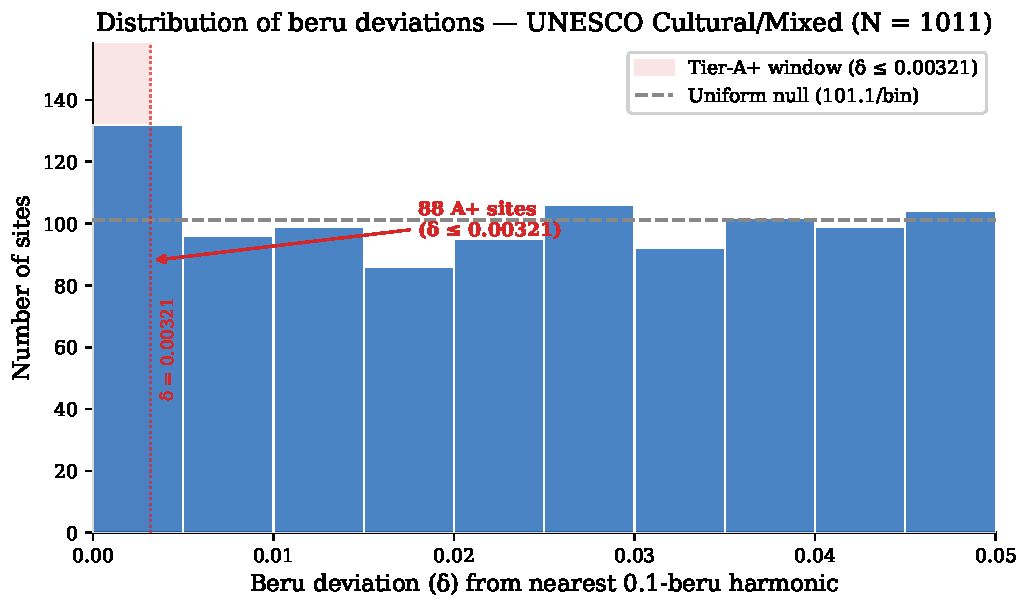
\includegraphics[width=0.9\textwidth]{../figures/fig_devhist}
\caption{Distribution of harmonic deviations for the full UNESCO corpus.
  The excess of sites within the Tier-A+ window ($\delta \leq \ApThreshDeg{}^\circ$,
  shaded) above the uniform null (dashed line) illustrates the corpus-level
  enrichment pattern; Tests~1 and~2 (domed monuments and cluster asymmetry)
  characterize its morphological and spatial structure.}
\label{fig:devhist}
\end{figure*}

The full UNESCO Cultural/Mixed corpus ($N = \NclusterTotal$) shows a
Tier-A+ rate of \clusterApRate\% (Figure~\ref{fig:devhist})
(\NclusterAp/\NclusterTotal; Clopper-Pearson 95\% CI
[\clusterApCIlo\%, \clusterApCIhi\%]),
above the \NullRateAp{} null
(binomial $p = \clusterApBinom$; supporting Test~4, not in the primary
diagnostic family).
The observed enrichment is $\clusterEnrichAp\times$, modest relative
to the dome subpopulation ($\circEnrichAp\times$) and the harmonic cluster
asymmetry. The primary threshold-free diagnostics are reported in
Table~\ref{tab:bonferroni_both}; they summarize structure within the
selected harmonic representation, not independent confirmation.

\textbf{Region-stratified audit.}
A region-specific empirical null (Fisher combination of per-region binomials)
yields $p = \pRegionEmpAll$ (\pRegionEmpAllSig{}), so it does not provide
region-stratified evidence against geographic concentration. The pre-2000
cohort remains elevated against the geometric null
($p = \pPreTwoK$~\pPreTwoKSig{}; \S\ref{sec:resultstemporal}), and is treated
as descriptive context.

\subsubsection*{World religion sites}
\label{sec:resultsrelig}
Religion sub-populations are defined by keyword sets documented in the supplementary audit archive~\citep{tenenbaum2026audit}.
A chi-squared test finds no significant A+ rate difference across the five main
religion groups ($\chi^2 = \religChiSqStat$, df\,=\,\religChiSqDof,
$p = \pReligChiSq$, \pReligChiSqSig{}).
Both Buddhism (\NbudATier/\NbudSitesRelig{} A-tier, \budATierRate\%;
\NbudInterHarmonic/\NbudSitesRelig{} C-band, \budInterHarmonicRate\%;
$p = \pBudJoint$~\pBudJointSig{}) and Hinduism (\NhinATier/\NhinSites{} A-tier, \hinATierRate\%;
\NhinInterHarmonic/\NhinSites{} C-band, \hinInterHarmonicRate\%;
$p = \pHinJoint$~\pHinJointSig{}) show a joint A-tier/C-band signal
(multivariate hypergeometric). Both persist in tradition-exclusive sites
($p = \pBudExclJoint$~\pBudExclJointSig{}, $p = \pHinExclJoint$~\pHinExclJointSig{}).

%------------------------------------------------------------------------------
\subsection{Domed and Spherical Monuments (Test~5, Supporting)}
\label{sec:resultscircular}

The keyword filter is described in \S\ref{sec:test_populations} ($N = \NcircTotal$).
The dome sub-corpus should be treated as a hypothesis-generating subpopulation:
the keyword set was refined iteratively during analysis, and the enrichment
should not be read as confirmatory evidence independent of that process.
\textbf{Test~1} (dome von~Mises mixture, Table~\ref{tab:bonferroni_both}): a two-component
von~Mises/uniform mixture with the mean fixed at the Gerizim phase yields
$\hat{w} = \targetedWdome$ ($\hat{\kappa} = \targetedKdome$),
$p_\mathrm{boot} = \targetedPdome$ (\targetedPdomeSig{};
Holm $p_\mathrm{adj} = \pHolmTestOne$, \pHolmTestOneSig{}).
Approximately $\targetedWdomePct\%$ of dome sites are concentrated at the Gerizim phase,
with an angular spread of ${\approx}\targetedSdDomeDeg$\textdegree{}.
The tier-based enrichment below provides complementary descriptive context.

\textbf{Tier-A++ concentration (supporting result).}
\NcircTierApp{} of \NcircTotal{} dome sites (\NcircAppRate\%, $\circEnrichApp\times$ the \NullRateApp{} null)
fall within Tier-A++ ($\delta \leq \AppThreshDeg{}^\circ$, $\lesssim\AppThreshKm{}$~km).
This concentration is directionally reproducible across three test statistics:
Fisher OR~$= \circAppFisherOR$, $p = \pCircAppFisher$~\pCircAppFisherSig{};
permutation $Z = \circAppPermZ$, $p = \circAppPermP$~\pCircAppPermSig{};
bootstrap $p = \circAppBootP$~\pCircAppBootSig{}.
Dome A++ gives consistent results across all three null models and remains directionally robust under full Bonferroni at $k = \NtotalTests$ (\S\ref{sec:multiple_comparisons}).

\textbf{Tier-A+ enrichment (supporting Test~5).}
\NcircTierAp/\NcircTotal{} sites at Tier-A+
(\NcircApRate\% [\circApCIlo, \circApCIhi], $\circEnrichAp\times$;
Fisher OR~$= \circApFisherOR$, $p = \pCircApFisher$~\pCircApFisherSig{};
binomial $p = \pCircAp$~\pCircApSig{}).
Tier-A: \NcircTierA/\NcircTotal{} (\circARate\%, $\circEnrichA\times$;
Fisher $p = \pCircAFisher$~\pCircAFisherSig{};
binomial $p = \pCircA$~\pCircASig{}).
The $\chi^2$-uniform test ($p = \pCircChi$, \pCircChiSig{}) is consistent with
concentration at harmonic nodes.
Tier-B (middle zone): \NcircTierB/\NcircTotal{} sites;
mean $\delta = \circMeanDev$\textdegree{}.

\noindent\textbf{Tier-A+ sites}:
Khoja Ahmed Yasawi (0.2~km),
Boyana Church (0.3~km),
Lumbini (0.8~km),
Humayun's Tomb (2.0~km),
Pyu Ancient Cities (2.3~km),
Silk Roads: Chang'an-Tianshan (2.5~km), Trulli of Alberobello (3.6~km),
Old City of Jerusalem (4.1~km),
Borobudur (4.3~km),
Kizhi Pogost (5.0~km), Echmiatsin/Zvartnots (6.2~km).

A leave-one-out binomial check shows that no single site drives the result:
removing any A+ site yields $N = \LOOdomeN$, A+$= \LOOdomeAp$,
$p = \LOOdomeP$.
Leave-2-out (worst case) across all $\binom{\LKOnAp}{2}$ combinations:
$p = \LKOworstTwoP$.
Leave-3-out (worst case): $p = \LKOworstThreeP$; the evolution corpus (Test~6) (\S\ref{sec:resultsevolution_inline}) 
and the A++ concentration are more robust. 
The A++ leave-3-out worst case across all
$\binom{\LKOAppNApp}{3} = \LKOAppNCombosThreeApp$ triples yields
$p = \LKOAppworstThreeP$, remaining below $\alpha = 0.05$ in this audit
(leave-2-out worst case $p = \LKOAppworstTwoP$).

\textbf{Multi-scale combined enrichment.}
\label{sec:multiscale}
A Fisher combination across \multiscaleK{} log-spaced proximity windows
(null rates 0.33\% to 40\%; canonical tiers A++, A+, A are three of the \multiscaleK{})
shows all windows enriched above their null (OR 1.2$\times$ to 6.7$\times$,
14 of 15 individually $p < 0.10$);
permutation-calibrated $p = \multiscaleDomeCombinedP$~\multiscaleDomeCombinedPSig{}.
No fixed tier cutoff enters this statistic.
Applied jointly across all four corpora (UNESCO domes, UNESCO full,
Wikidata Q180987 stupas, OWTRAD Silk Road vertices), the maximum joint enrichment
falls at approximately \multiscaleJointMaxKm{} km from a harmonic node
(1/10th of the \textasciitilde{}289 km inter-node spacing at 30\textdegree{}N),
with permutation-calibrated $p = \multiscaleJointMaxP$~\multiscaleJointMaxPSig{}.
Each corpus peaks within this \multiscaleJointMaxKm{} km bound
(4 to 29 km across corpora), a scale that emerges from the data rather than any
pre-specified threshold.

\textbf{Context-validated robustness (Test~5x).}
Sentence-level validation ($N = \NcircValidated$, \NcircContextRejected{} rejected):
A++ $p = \pCircAppValidatedFisher$~\pCircAppValidatedFisherSig{};
A+ $p = \pCircApValidatedFisher$~\pCircApValidatedFisherSig{}.
The A++ result strengthens when false positives are removed; A+ remains
directionally elevated under this stricter filter.
Keyword-stratified check: stupa/stupas alone ($n = \kwSensStupaN$) carries the strongest signal
(A++ $p = \kwSensStupaAppP$~\kwSensStupaAppPSig{});
dome/tholos/spherical without stupa ($n = \kwSensNoStupaN$) remains elevated
($p = \kwSensNoStupaAppP$~\kwSensNoStupaAppPSig{}).

\textbf{Geographic-concentration checks (dedicated simulation).}
\label{sec:geo_conc_null}
Domed monuments are concentrated in the Eurasian corridor:
\domeEurasianFraction\% fall in 20\textdegree{} to 120\textdegree{}E
versus \fullCorpusEurasianFraction\% of the full corpus.
Two targeted resampling checks evaluate whether this explains the dome enrichment
(\simNperms{} trials).

\textbf{Null~A (within-dome bootstrap stability check):} Draw $N = \NcircTotal$ longitudes
from the dome sites' own list. Mean $= \geoNullDomeBootMean$ A+,
$p = \geoNullDomeBootP$ (\geoNullDomeBootPSig{}). The dome sites' positions are concentrated
near harmonic longitudes; this check characterizes the observed dome
distribution rather than serving as an external geographic null.

\textbf{Null~C (restricted geographic-concentration null):} Pool all full-corpus sites
within $\pm W$\textdegree{} of any dome site and bootstrap the expected A+
count. Dome sites (\NcircTierAp~A+, \NcircApRate\%) exceed
the broader footprint at all three windows tested:
$\pm 2$\textdegree{} ($p = \geoNullDomeRestrictedPtwo$, \geoNullDomeRestrictedPtwoSig{});
$\pm 5$\textdegree{} ($p = \geoNullDomeRestrictedP$, \geoNullDomeRestrictedPSig{});
$\pm 10$\textdegree{} ($p = \geoNullDomeRestrictedPten$, \geoNullDomeRestrictedPtenSig{}).
Results are stable across the tested window widths.


\begin{figure*}[!t]
\centering
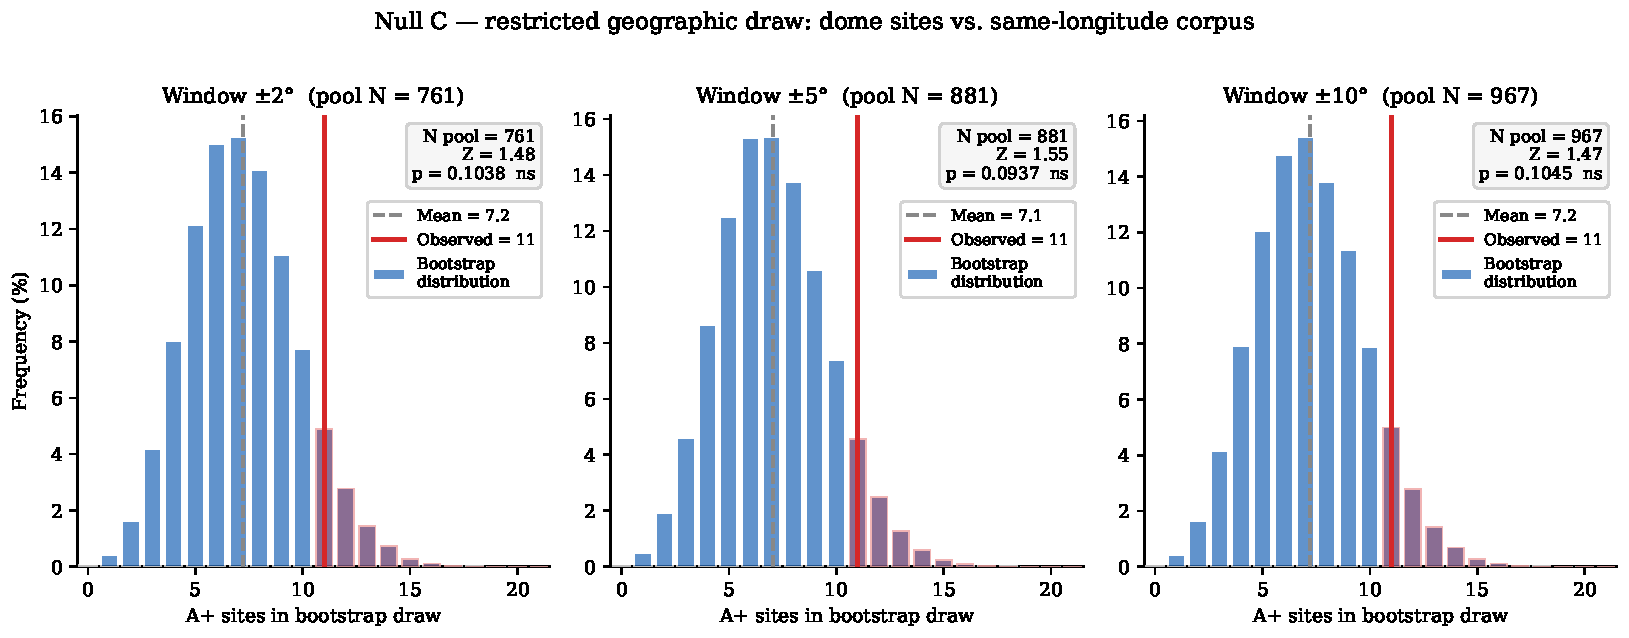
\includegraphics[width=0.9\textwidth]{../figures/fig_null_c}
\caption{Null~C bootstrap distributions for the dome sub-population
  ($N = \NcircTotal$, observed A+ $= \NcircTierAp$) at three
  window widths. For each window $\pm W$\textdegree{}, all full-corpus
  sites within $\pm W$\textdegree{} of any dome longitude form the
  restricted pool; $10^5$ draws of size $N = \NcircTotal$ from that
  pool define the expected A+ distribution (blue bars). The observed
  count (red line) exceeds the pool mean by $Z \approx 2.7$ in all three
  windows ($\pm 2$\textdegree{}: $p = \geoNullDomeRestrictedPtwo$, \geoNullDomeRestrictedPtwoSig{};
  $\pm 5$\textdegree{}: $p = \geoNullDomeRestrictedP$, \geoNullDomeRestrictedPSig{};
  $\pm 10$\textdegree{}: $p = \geoNullDomeRestrictedPten$, \geoNullDomeRestrictedPtenSig{}),
  showing stability across the tested window widths.}
\label{fig:null_c}
\end{figure*}

In the global anchor sweep (\S\ref{sec:sensitivity_global}),
Gerizim scores \GerizimSweepAp{} A+ (\anchorSweepPctile{}\textsuperscript{th}
percentile); Jerusalem scores \JerusalemSweepAp{}
(\JerusalemSweepPctile{}\textsuperscript{th}).

\subsection{Hemispherical Mound Evolution (Test~6, Sensitivity)}
\label{sec:resultsevolution_inline}

Extending the dome keyword subset of Test~5 with earthen mound-stage keywords (see \S\ref{sec:test_populations});
the combined population ($N = \NevoTotal$) adds
\NevoMoundOnly{} mound-stage sites to the core
domed/spherical population, with \NevoOverlap{}
sites matching both keyword sets.

\noindent\textbf{Stage-by-stage breakdown} (Table~\ref{tab:evostages1b}):

\begin{table*}[!t]
\centering
\caption{Test~6 enrichment by evolutionary stage ($N = \NevoTotal$).
  Null rates: A++~$P_0 = \NullRateApp{}$, A+~$P_0 = \NullRateAp{}$, A~$P_0 = \NullRateA{}$.
  Fisher exact tests: stage vs.\ full corpus background.}
\label{tab:evostages1b}
\small
\adjustbox{max width=\textwidth}{%
\begin{tabular}{lrrllrllrl}
\toprule
 & & \multicolumn{2}{c}{Tier~A++ ($\leq\AppThreshKm{}$\,km)} & & \multicolumn{2}{c}{Tier~A+ ($\leq\ApThreshKm{}$\,km)} & & \multicolumn{2}{c}{Tier~A ($\leq\ATierThreshKm{}$\,km)} \\
\cmidrule(lr){3-4}\cmidrule(lr){6-7}\cmidrule(lr){9-10}
Stage & $N$ & A++ & Rate OR ($p$) & & A+ & Rate OR ($p$) & & A & Rate OR ($p$) \\
\midrule
Mound\textsuperscript{a} & \NevoMound
  & \NevoMoundApp & \evoMoundAppRate\% $\evoMoundAppFisherOR\times$ (\pEvoMoundAppFisher~\pEvoMoundAppFisherSig{}) &
  & \NevoMoundAp  & \evoMoundApRate\%  $\evoMoundFisherOR\times$ (\pEvoMoundFisher~\pEvoMoundFisherSig{}) &
  & \NevoMoundA   & \evoMoundARate\%   $\evoMoundAFisherOR\times$ (\pEvoMoundAFisher~\pEvoMoundAFisherSig{}) \\
Stupa\textsuperscript{b} & \NevoStupa
  & \NevoStupaApp & \evoStupaAppRate\% $\evoStupaAppFisherOR\times$ (\pEvoStupaAppFisher~\pEvoStupaAppFisherSig{}) &
  & \NevoStupaAp  & \evoStupaApRate\%  $\evoStupaFisherOR\times$ (\pEvoStupaFisher~\pEvoStupaFisherSig{}) &
  & \NevoStupaA   & \evoStupaARate\%   $\evoStupaAFisherOR\times$ (\pEvoStupaAFisher~\pEvoStupaAFisherSig{}) \\
Dome\textsuperscript{c}  & \NevoDome
  & \NevoDomeApp  & \evoDomeAppRate\%  $\evoDomeAppFisherOR\times$ (\pEvoDomeAppFisher~\pEvoDomeAppFisherSig{}) &
  & \NevoDomeAp   & \evoDomeApRate\%   $\evoDomeFisherOR\times$ (\pEvoDomeFisher~\pEvoDomeFisherSig{}) &
  & \NevoDomeA    & \evoDomeARate\%    $\evoDomeAFisherOR\times$ (\pEvoDomeAFisher~\pEvoDomeAFisherSig{}) \\
\midrule
\textbf{Combined} & \textbf{\NevoTotal}
  & \textbf{\NevoApp} & \textbf{\evoAppRate\%} $\mathbf{\evoAppFisherOR\times}$ (\textbf{\pEvoAppFisher~\pEvoAppFisherSig{}}) &
  & \textbf{\NevoAp}  & \textbf{\evoApRate\%}  $\mathbf{\evoApFisherOR\times}$ (\textbf{\pEvoApFisher~\pEvoApFisherSig{}}) &
  & \textbf{\NevoA}   & \textbf{\evoARate\%}   $\mathbf{\evoAFisherOR\times}$ (\textbf{\pEvoAFisher~\pEvoAFisherSig{}}) \\
\bottomrule
\multicolumn{10}{p{1.2\linewidth}}{\footnotesize
  \textsuperscript{a}tumulus/barrow/kofun.\;
  \textsuperscript{b}stupa/stupas.\;
  \textsuperscript{c}dome/tholos/spherical.
  OR = odds ratio; $p$ = one-sided Fisher exact vs.\ full UNESCO cultural corpus ($N = \NclusterTotal$).
  Stage $N$ values sum to more than the combined total because \NevoOverlap{} sites match multiple stages.} \\
\end{tabular}}
\end{table*}

\noindent The combined population ($N = \NevoTotal$, A+ = \evoApRate\%;
Table~\ref{tab:evostages1b}) is consistent with Test~1. The mound stage does not reach
significance (\evoMoundApRate\%, OR $= \evoMoundFisherOR\times$, Fisher $p = \pEvoMoundFisher$, \pEvoMoundFisherSig{}). The signal is carried
by the stupa (A+ \evoStupaApRate\%, OR $= \evoStupaFisherOR\times$, $p = \pEvoStupaFisher$~\pEvoStupaFisherSig{}) and dome
sub-stages (A+ \evoDomeApRate\%, OR $= \evoDomeFisherOR\times$, $p = \pEvoDomeFisher$~\pEvoDomeFisherSig{}).
Leave-one-out checks confirm stability.
Leave-3-out (worst case, $\EvoLKOnCombosThree{}$ triples):
$p = \EvoLKOworstThreeP$.

\textbf{Stupa geographic-concentration null.}
\label{sec:stupa_geo_null}
Stupa sites are concentrated in South/Southeast Asia
(\stupaHeartlandFrac\% in 70\textdegree{} to 110\textdegree{}E).
Null~A (within-stupa bootstrap): $p = \stupaGeoBootP$ (\stupaGeoBootPSig{}).
Null~C (restricted $\pm 5$\textdegree{} draw): $p = \stupaGeoRestrictedP$ (\stupaGeoRestrictedPSig{}).

\subsection{Temporal Gradient (Test~7, Descriptive)}
\label{sec:resultstemporal}

The Tier-A++ rate in the founding canon (1978 to 1984) is \cohortAppArate\%
(\NcohortAppAapp/\NcohortAppA{}; $\canonEnrich\times$ the \NullRateApp{} null,
$p = \pCanonApp$~\pCanonAppSig{}), declining monotonically toward the null
in later cohorts (2000 to 2025: \cohortAppErate\%).
Cochran-Armitage three-cohort trend test (A++, decreasing):
$Z = \ZcochranAppThree$, $p = \pCochranAppThree$~(\pCochranAppThreeSig{}).
The five-cohort trend is marginal ($p = \pCochranAppFive$~\pCochranAppFiveSig{}).
By contrast, the A+ rate shows no significant decreasing trend
($p = \pCochranThree$~\pCochranThreeSig{}), consistent with the gradient
being specific to the highest-precision tier.
This is consistent with UNESCO's founding canon over-representing
historically prominent monuments, some of which are also precisely aligned
to harmonic nodes.
The Mantel-Haenszel stratified test is underpowered at the sub-group level;
Logistic regression with region as a covariate is directionally consistent
with the A++ gradient
($Z = \zLogRegCohortApp$, $p = \pLogRegCohortApp$~\pLogRegCohortAppSig{},
OR~$= \orLogRegCohortApp$).
The declining rate may partly reflect UNESCO's expansion into regions where hemispherical traditions are less prevalent.
The gradient is treated as descriptive context only (Figure~\ref{fig:temporal}).

\begin{figure*}[!t]
\centering
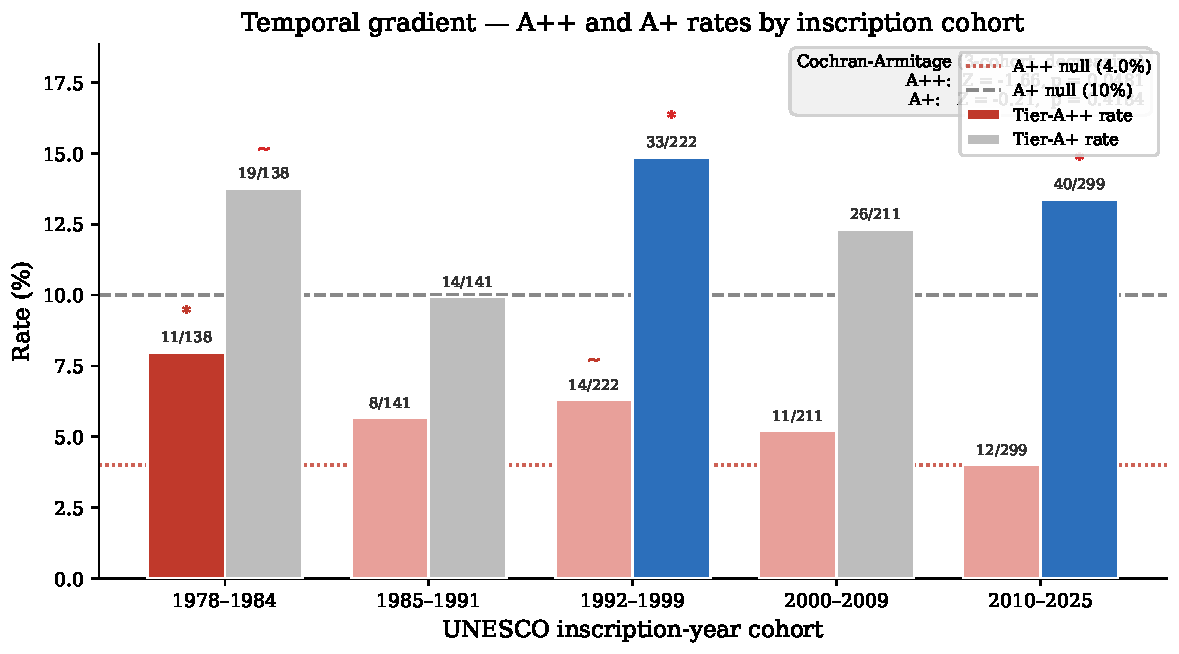
\includegraphics[width=0.9\textwidth]{../figures/fig_temporal}
\caption{Tier-A++ and Tier-A+ rates by UNESCO inscription-year cohort.
  The founding canon (1978 to 1984) shows an elevated A++ rate
  (\cohortAppArate\%, $p = \pCanonApp$~\pCanonAppSig{}) that declines
  monotonically across later cohorts toward the \NullRateApp{} null (dotted line;
  Cochran-Armitage $Z = \ZcochranAppThree$, $p = \pCochranAppThree$~\pCochranAppThreeSig{}).
  The A+ rate (right bars) shows no significant trend ($p = \pCochranThree$~\pCochranThreeSig{}).}
\label{fig:temporal}
\end{figure*}

\begin{table*}[tp]
\centering\small
\caption{Multiple-comparisons summary.
  Primary diagnostic family: Tests~1 to~3 (threshold-free, $k = \BonfK$).
  Supporting enrichment tests (Tests~4 and~5) use a pre-specified $p_0 = \NullRateAp{}$
  proximity window; see \S\ref{sec:enrichment_tests}.}
\label{tab:bonferroni_both}
\adjustbox{max width=\textwidth}{%
\begin{tabular}{lcrll}
\toprule
Test & $N$ & Raw $p$ & Holm $p_\mathrm{adj}$, $k{=}\BonfK$ & Status \\
\midrule
Test~1 (dome VM mix.)  & \NcircTotal     & \targetedPdome$^{b}$ ($w = \targetedWdome$, $\kappa = \targetedKdome$) & \pHolmTestOne~\pHolmTestOneSig{}  & \textbf{Diagnostic} \\
Test~2 (Spearman)      & \NclusterTotal  & \spearmanDevClusterP$^{b}$ ($\rho = \spearmanDevClusterRho$) & \pHolmTestTwo~\pHolmTestTwoSig{}  & \textbf{Diagnostic} \\
Test~3 (mean dev.)     & \NclusterTotal  & \fullMeanDevPermP$^{b}$ & \pHolmTestThree~\pHolmTestThreeSig{} & \textbf{Diagnostic} \\
\midrule
Test~4 (full-corpus A+) & \NclusterTotal & \clusterApBinom$^{a}$ & N/A  & Supporting \\
Test~5 (dome A+)        & \NcircTotal    & \pCircAp$^{a}$ (OR~$= \circApFisherOR$) & N/A & Supporting \\
Test~6 (mound evol.)   & \NevoTotal      & \pEvoApFisher$^{a}$ (OR~$= \evoApFisherOR$) & N/A  & Sensitivity \\
\midrule
Test~7 (temporal)      & \NoriginCorpus  & \pCochranThree$^{b}$ & N/A  & Descriptive \\
\bottomrule
\multicolumn{5}{p{0.95\textwidth}}{\footnotesize
  $^{a}$Binomial or Fisher exact $p$ vs.\ $\NullRateAp{}$ geometric null (window $= \ApThreshDeg{}^\circ$; convenience choice, sensitivity-audited over $2\%$ to $10\%$ null rates in Supplementary~S1);
  $^{b}$permutation or bootstrap $p$.
  Tests~1 to~3 are threshold-free; no tier cutoff enters any primary diagnostic.
  Adjusted $p$-values describe calibration within the selected representation,
  not confirmatory rejection of a global discovery null.
  Holm (1979) step-down \citep{holm1979simple}.} \\
\end{tabular}}
\end{table*}

\subsection{FDR audit and Bonferroni correction}
\label{sec:fdraudit}

Results are consolidated in Table~\ref{tab:bonferroni_both}.
A comprehensive FDR audit (\NtotalTests{} tests;
\citealt{benjamini1995controlling}) retains \NsurviveFDR{} at $q < 0.05$;
\NsurviveBonfAll{} remain below the full-Bonferroni audit threshold at $k = \NtotalTests$:
dome/spherical A++ ($p = \BonfAllSurvivepCircApp$),
cluster permutation ($p = \BonfAllSurviveclusterPermP$),
harmonic Mann-Whitney ($p = \BonfAllSurviveclusterHarmonicMWp$),
sequential-peak permutation ($p = \BonfAllSurvivepeakSigP$),
and evolution combined A++ ($p = \BonfAllSurvivepEvoApp$).

\section{Robustness Checks}
\label{sec:robustness}

\subsection{Unit Sweep and Sensitivity Slope}
\label{sec:metrology}

Unit sweep and sensitivity slope results are in \S\ref{sec:results_unit_sweep}.
Briefly: nearby non-harmonic spacings are non-significant; a $\pm 0.3\%$
shift collapses joint significance; Monte Carlo sweep
(\S\ref{sec:limitations_geo}) supports the relative peak;
Tests~C and~D (\S\ref{sec:results_rayleigh}) support phase specificity
within the selected 3\textdegree{} frame.

\subsection{Global Anchor Sweep}
\label{sec:sensitivity_global}

The global sweep (\anchorSweepNanchors{} trial anchors, 0.01\textdegree{}
resolution) uses the full corpus plus synthetic Gerizim
(\S\ref{sec:geodetic}), with each anchor self-excluding
($N = \NgerizimSweepCorpus$ per trial).

Both anchors place the corridor in the global top \anchorSweepTopPct\%
(\anchorSweepNanchors{} trial anchors, 0 to 360\textdegree{}E;
Gerizim: \GerizimSweepAp{} A+, \anchorSweepPctile\textsuperscript{th} percentile;
Jerusalem: \JerusalemSweepAp{} A+, \JerusalemSweepPctile\textsuperscript{th}
percentile). The result is anchor-invariant within the
\GerizimJerusalemKm\,km corridor window.
Other historical meridians tested here do not show comparable enrichment.

\subsubsection*{The 35.25\textdegree{}E modulo-3\textdegree{} phase band}
\label{sec:phase_peak_artifact}

Every longitude congruent to 35.25\textdegree{}E modulo 3\textdegree{}
(\NharmonicsCoarse{} anchors)
produces identically the maximum A+ count, spaced 3\textdegree{} apart.
The flat-top width is a function of the tier threshold chosen:
A++ ($\pm\AppThreshDeg{}^\circ$), A+ ($\pm\ApThreshDeg{}^\circ$), A ($\pm\ATierThreshDeg{}^\circ$);
the number of tied anchors is a methodological artifact, not a physical feature.
Mount Gerizim is a fixed landmark at \GerizimLon\textdegree{}E (phase $\GerizimPhase$\textdegree{},
gap $\phaseGap$\textdegree{} $\approx \phaseGapKm$~km). It lies within the A and A+ flat-top
bands but not A++.

\subsubsection*{Formal statistical tests for the 35.25\textdegree{}E modulo-3\textdegree{} phase band}
\label{sec:phase_peak_formal}

The full-corpus Rayleigh ($p_\mathrm{perm} = \fullRayleighPermP$, \fullRayleighPermPSig{}) shows no
global 3\textdegree{} spectral periodicity; Test~B is tautological.
Tests~C ($p_\mathrm{perm} = \anchorShiftPermP$, \anchorShiftPermPSig{}) and~D ($p_\mathrm{boot} = \targetedPfull$, \targetedPfullSig{})
are positive anchor-specific tests; Test~E ($p = \anchorMaxPermP$, \anchorMaxPermPSig{}, marginal) is the anchor discovery correction.
The unit sensitivity sweep (\S\ref{sec:metrology}) and Monte Carlo unit sweep
(\S\ref{sec:limitations_geo}) identify 3\textdegree{} as the highest-scoring
spacing under the template score, \emph{given} the pre-specified Gerizim anchor;
neither sweep constitutes anchor-free or period-free discovery.

\textbf{Corridor and landmark ranking.}
Of the \corridorUniqueGer{} A+ sites unique to Gerizim and
\corridorUniqueJer{} unique to Jerusalem, \corridorSharedAp{} are shared;
the enrichment belongs to the corridor, not to either anchor individually.
Using each UNESCO site as anchor, Gerizim ranks
\#\GerizimTempleRank{} among the extended candidate landmarks
(\GerizimPctileAp\textsuperscript{th} percentile).

\subsection{Spatial Autocorrelation}
\label{sec:autocorrelation}

A+ harmonics host $\clusterHarmonicRatio\times$ as many total UNESCO
sites as non-A+ harmonics ($p\ \clusterHarmonicMWpStr$).
DEFF correction via ICC ($\pm 0.5$\textdegree{}, $\rho = \ICChalf$):
DEFF~$= \DEFFhalf$, $N_\mathrm{eff} = \NeffHalf$,
corrected $p = \pNeffHalf$.
Block bootstrap (3\textdegree{} blocks, \simNperms{} resamples):
95\% CI $[\blockBootCIlo\%, \blockBootCIhi\%]$ excludes the \NullRateAp{} null.
Within-group permutation is non-discriminating for alignment vs.\ geographic
concentration; the restricted geographic-concentration null
(\S\ref{sec:geo_conc_null}) addresses that comparison directly.

\subsection{Null Model Validation}
\label{sec:simulation_null}

Three simulation nulls (\simNperms{} trials each, seed~$= \simSeed{}$,
\citealt{good2005permutation}):
(1)~Longitude permutation: dome ($N = \NcircValidated$)
$p_\mathrm{perm} = \simDomePermP$~\simDomePermPSig{};
1978-1984 canon ($N = \NcanonSites$) $p = \simCanonPermP$~\simCanonPermPSig{};
pre-2000 ($N = \NpreTwoK$) $p = \simPreTwoKPermP$~\simPreTwoKPermPSig{}.
(2)~Bootstrap from full corpus: dome $p_\mathrm{boot} = \simDomeBootP$~\simDomeBootPSig{}.
(3)~KDE-smoothed null: expected $\simKDEMean \pm \simKDEStd$, observed \Nap{}, $Z = \simKDEZ$,
$p = \simKDEP$~\simKDEPSig{}.
The KDE null ($p = \simKDEP$~\simKDEPSig{}) supports dome enrichment; permutation and bootstrap
are marginal at the A+ level but stronger for the A++ sub-population
(permutation $p = \circAppPermP$~\pCircAppPermSig{},
bootstrap $p = \circAppBootP$~\pCircAppBootSig{}).
The within-dome bootstrap characterizes the observed concentration near
harmonic longitudes, while the restricted geographic-concentration null
(Null~C; \S\ref{sec:geo_conc_null}) indicates that longitude footprint
alone is not sufficient to explain the dome enrichment.

\subsection{Pipeline Portability: Wikidata Q180987 Stupa Corpus}
\label{sec:stupas_q180987}

The pipeline was applied to $N = \wikiStupaTotal{}$ Wikidata-attested stupas
(class Q180987) in a separately assembled corpus \citep{tenenbaum2026audit}.
The Kedu Plain (Java) hosts the densest cluster at the 75\textdegree{} harmonic (75\textdegree{}E from Gerizim),
anchored by Borobudur (c.\ 800~CE, \wikiStupaBorobudurDevKm~km, Tier~A+)
\citep{miksic1990borobudur}; the World Peace Pagoda at Lumbini achieves
A++ precision ($\sim$\wikiStupaLumbiniDevM~m) under the Gerizim reference
frame.

Using the identical anchor and null, the corpus yields
\wikiStupaATierCount/\wikiStupaTotal{} Tier-A sites
(\wikiStupaATierRate\%, $\wikiStupaATierEnrich\times$ null;
binomial $p\ \wikiStupaATierBinomP$, \wikiStupaATierBinomStar;
permutation $Z = \wikiStupaPermZ$, $p_\mathrm{perm} = \wikiStupaPermP$,
\wikiStupaPermStar).
Tier-A+ is nominally elevated under the simple binomial count
(\wikiStupaApCount/\wikiStupaTotal{}, \wikiStupaApRate\%,
binomial $p = \wikiStupaApBinomP$~\wikiStupaApBinomStar), but the
portable signal is strongest at Tier-A because this external-corpus
analysis ranks cluster-level occupancy rather than individual-site
precision. Its tier emphasis should therefore not be read as mechanically
identical to the UNESCO dome scoring.
Harmonic nodes with at least one Tier-A site carry $\wikiStupaClusterRatio\times$
more stupa sites on average than empty nodes, mirroring the cluster-asymmetry
result of Test~3.

\textbf{Geographic tier breakdown and bimodal structure.}
All regional p-values below are one-sided Fisher exact tests.
A sub-regional breakdown reveals a bimodal pattern consistent with the
Buddhist and Hindu bimodal enrichment in the UNESCO religion audit (\S\ref{sec:resultsrelig}).
The Java/Sumatra node (105\textdegree{} to 115\textdegree{}E, near the 75\textdegree{} harmonic at 110.3\textdegree{}E)
concentrates \wikiJavaNodeATierN{} of \wikiJavaNodeN{} sites at Tier-A (\wikiJavaNodeATierRate\%, OR $= \wikiJavaNodeATierOR\times$, $p~\wikiJavaNodeATierP$~\wikiJavaNodeATierPSig{}),
rising to \wikiJavaTightATierN/\wikiJavaTightN{} (\wikiJavaTightATierRate\%, OR $= \wikiJavaTightATierOR\times$, $p~\wikiJavaTightATierP$~\wikiJavaTightATierPSig{}) in the 107\textdegree{} to 112\textdegree{}E window,
where A+ is also elevated at \wikiJavaTightApRate\% (OR $= \wikiJavaTightApOR\times$, $p\ \wikiJavaTightApP$~\wikiJavaTightApPSig{}).
The physical heartland, India/Nepal (70\textdegree{} to 90\textdegree{}E) and Myanmar/Cambodia
(90\textdegree{} to 105\textdegree{}E), is A-tier depleted (combined OR $= \wikiHeartlandATierOR\times$,
$p~\wikiHeartlandATierP$~\wikiHeartlandATierPSig{}, one-sided depletion test)
but strongly enriched in the inter-harmonic C-band:
Myanmar/Cambodia reaches \wikiMyanmarCbandRate\% (OR $= \wikiMyanmarCbandOR\times$, $p~\wikiMyanmarCbandP$~\wikiMyanmarCbandPSig{}) and the
combined heartland \wikiHeartlandCbandRate\% (OR $= \wikiHeartlandCbandOR\times$, $p~\wikiHeartlandCbandP$~\wikiHeartlandCbandPSig{}).
This A/C anti-correlation mirrors the bimodal pattern in the religion audit (\S\ref{sec:resultsrelig}).
Non-heartland Wikidata stupas (outside 70\textdegree{} to 110\textdegree{}E,
$N = \wikiNonHeartlandN{}$) show the same A-enriched, C-depleted profile:
\wikiNonHeartlandATierRate\% reach Tier-A (OR $= \wikiNonHeartlandATierOR\times$, $p~\wikiNonHeartlandATierP$~\wikiNonHeartlandATierPSig{})
with no C-band enrichment (OR~$= \wikiNonHeartlandCbandOR\times$, $p = \wikiNonHeartlandCbandP$~\wikiNonHeartlandCbandPSig{}).

\subsection{Multiple Comparisons}
\label{sec:multiple_comparisons}

See \S\ref{sec:bonferroni} for the full protocol.
Gerizim ranks at the \anchorSweepPctile{}\textsuperscript{th} percentile;
a $\pm 0.3\%$ unit shift collapses joint significance.
FDR audit (\NtotalTests{} tests) retains \NsurviveFDR{} at $q < 0.05$;
\NsurviveBonfAll{} remain below the Bonferroni audit threshold at $k = \NtotalTests$.

\section{Limitations}
\label{sec:limitations}

\subsection{Exploratory Status and Multiple-Comparisons Exposure}
\label{sec:limitations_circularity}
\label{sec:circularity}

The analysis is exploratory: spacing, phase, anchor, sub-corpus, and tier
thresholds were all examined iteratively on a public dataset for which
prospective constraint is not applicable. The Holm correction covers only
the three primary diagnostics; $p$-values are descriptive, not confirmatory.
They are not tests of discovery. They quantify how sharply the selected
representation describes the data.
Key degrees of freedom (3\textdegree{} spacing, Gerizim phase, keyword set,
tier thresholds) have external motivation; threshold sensitivity is in
Supplementary~S1. External corpora are not independent of UNESCO
(\S\ref{sec:transmission}).

\subsection{Geographic and Cultural Selection Bias}
\label{sec:limitations_geo}

The UNESCO list over-represents Europe and the Mediterranean-to-South-Asian
corridor (Europe/N.~America \CorpusPctEurope\%; Arab States \CorpusPctArabStates\%;
Asia-Pacific \CorpusPctAsiaPac\%; Latin America \CorpusPctLatAm\%; Africa \CorpusPctAfrica\%).
Domed monuments exceed the A+ rate of other monuments from the same longitude
footprint (Null~C, $p = \geoNullDomeRestrictedP$, \geoNullDomeRestrictedPSig{}),
which indicates that architectural type may contribute to the enrichment beyond
longitude footprint alone.

A Monte Carlo unit sweep (\mcNperms{} permutations, \mcNcandidates{} candidate
spacings 0.5\textdegree{} to 15\textdegree{}) gives the highest template score
at 3\textdegree{} ($p < 0.001$), with harmonics at 6\textdegree{} and
12\textdegree{} also elevated under the same score.
The dome subset yields \mcDomeNsigCollapsed{} independent high-scoring spacing
($P = \mcDomeCollapsedPEqOne{}$ under the geographic null).

\subsection{Representation Dependence}
\label{sec:repn_dependence}

The observed structure depends on the representation. It is recovered under
nearest-harmonic-deviation scoring but not by invariant spectral methods
(no Rayleigh peak at 3\textdegree{} in any sub-corpus).
Three converging diagnostics: (i)~a $\pm 0.3\%$ unit perturbation
collapses joint significance (\S\ref{sec:results_unit_sweep});
(ii)~multi-scale enrichment is broad, not a sharp spectral line;
(iii)~the anchor-sweep maximum is marginal ($p = \anchorMaxPermP$,
\anchorMaxPermPSig{}) while targeted tests at the identified frame
are stronger (\S\ref{sec:sensitivity_global}).
The pattern appears under the representation, not as intrinsic
periodicity. It arises from the interaction between the scoring function
and the imposed coordinate frame.
A clustered control shows that the unconstrained global maximum over
all $(\omega,\phi)$ is typical under realistic dome-site clustering
($p = \clusterCtrlPermP$, $N_{\mathrm{sim}} = \clusterCtrlNsim$) and does
not uniquely recover the hypothesised frame.
The free-sweep maximizer returns $\omega = \clusterCtrlObsOmega$\textdegree{},
a spacing with no metrological or waypoint interpretation, confirming
that the unconstrained maximum reflects spatial clustering rather than
any meaningful periodicity.
This outcome is expected: the enrichment statistic uses a fixed absolute
threshold (0.15\textdegree{}), so large spacings receive an artificially
low null rate and therefore inflate the enrichment ratio regardless of
any real structure. The free sweep is uninformative precisely because it
is not scale-invariant; the metrologically motivated prior $\omega = 3$\textdegree{}
is tested conditionally, not recovered by unconstrained search.

\subsection{Americas Negative Control}
\label{sec:americas_negative_control}
The UNESCO Americas sub-corpus ($N = \AmericasN$) shows A+ rate
\AmericasApRate\%, below the \NullRateAp{} null
($p = \AmericasOneSidedP$~\AmericasOneSidedStar{}, one-sided depletion).

\subsection{Other Limitations}

\textbf{Geocoding precision.}
UNESCO XML coordinates are administrative centroids (unsystematic noise, no directional bias).

\textbf{Metrological evidence.}
The 3\textdegree{} template was initially motivated as a base-10 subdivision
of the 30\textdegree{} b\={e}ru \citep{hunger2019mul,powell1987metrological}.
No ancient surveying instrument calibrated to such sub-units has been
recovered, and the metrological parallel is treated as heuristic motivation,
not evidence. All thresholds are degree-denominated.

%------------------------------------------------------------------------------
\section{Discussion}
\label{sec:discussion}

\subsection{Template Alignment vs.\ Intrinsic Periodicity}
\label{sec:template_vs_intrinsic}

The present results are best treated as \emph{template alignment}
(\S\ref{sec:repn_dependence}): a reproducible, phase-localized pattern
appears under the representation but is not invariant and does not imply a
periodic generative model. The analysis does not demonstrate an underlying
spatial law or intentional placement. It shows that coordinate-aligned
statistics can produce reproducible deviations in clustered datasets.
Interpretation should focus on properties of the representation, not the
existence of a latent periodic structure.

\subsection{Alternative Explanations}
\label{sec:alt_explanations}

\textbf{(1) Independent convergence.}
Hemispherical structures recur across cultures
\citep{aveni2001skywatchers,aveni2003archaeoastronomy}, but convergence
predicts no longitude specificity.

\textbf{(2) Geographic concentration.}
Null~C: other monuments from the same longitude footprint are less
enriched than the dome subset ($p = \geoNullDomeRestrictedP$,
\geoNullDomeRestrictedPSig{}); these checks reduce, but do not eliminate,
the possibility that enrichment partly reflects corridor concentration.

\textbf{(3) Random coincidence.}
Simulation nulls (KDE, permutation, bootstrap) support dome enrichment within
the selected representation,
most strongly at A++ (permutation $p = \circAppPermP$~\pCircAppPermSig{};
full results in \S\ref{sec:simulation_null}).
Tests~C and~D support phase specificity within the selected frame
(\S\ref{sec:results_rayleigh}).

\subsection{Cross-Corpus Consistency: OWTRAD and Wikidata}
\label{sec:transmission}

Two additional corpora (the Wikidata Q180987 stupa inventory and the
OWTRAD route network \citep{ciolek2004owtrad}) are analyzed under the
same harmonic-deviation representation. These datasets are not statistically
independent of the UNESCO corpus, as they share geographic and cultural
structure. Their role here is not replication, but to assess whether the
observed alignment behavior is stable across related datasets under a
common representation.

\textbf{OWTRAD route network.} The OWTRAD route network contains
\NOwtradEdges{} route segments and \NOwtradVertices{} unique endpoints.
Under the same representation, the degree-weighted endpoint distribution
shows A++ enrichment (\NOwtradDegWApp{} of \NOwtradDegW{} endpoint positions,
$z = \zOwtradDegWApp$, $p\ \pOwtradDegWApp$~\pOwtradDegWAppSig{}), while the deduplicated endpoint
distribution is weaker (\NOwtradVertexApp{}/\NOwtradVertices{}, $p =
\pOwtradVertexApp$~\pOwtradVertexAppSig{}). A phase-shift test gives
$p = \pOwtradVertexAppPhase$~\pOwtradVertexAppPhaseSig{}, and a
cluster-asymmetry check gives $p = \pOwtradClustDeg$~\pOwtradClustDegSig{}.
These results are treated as shared-representation consistency, not
independent replication. The Silk Road corridor is illustrated in
Figure~\ref{fig:geo_trail}; harmonic tier distributions for both OWTRAD
populations are shown in Figure~\ref{fig:owtrad_tiers}.

\begin{figure*}[!t]
  \centering
  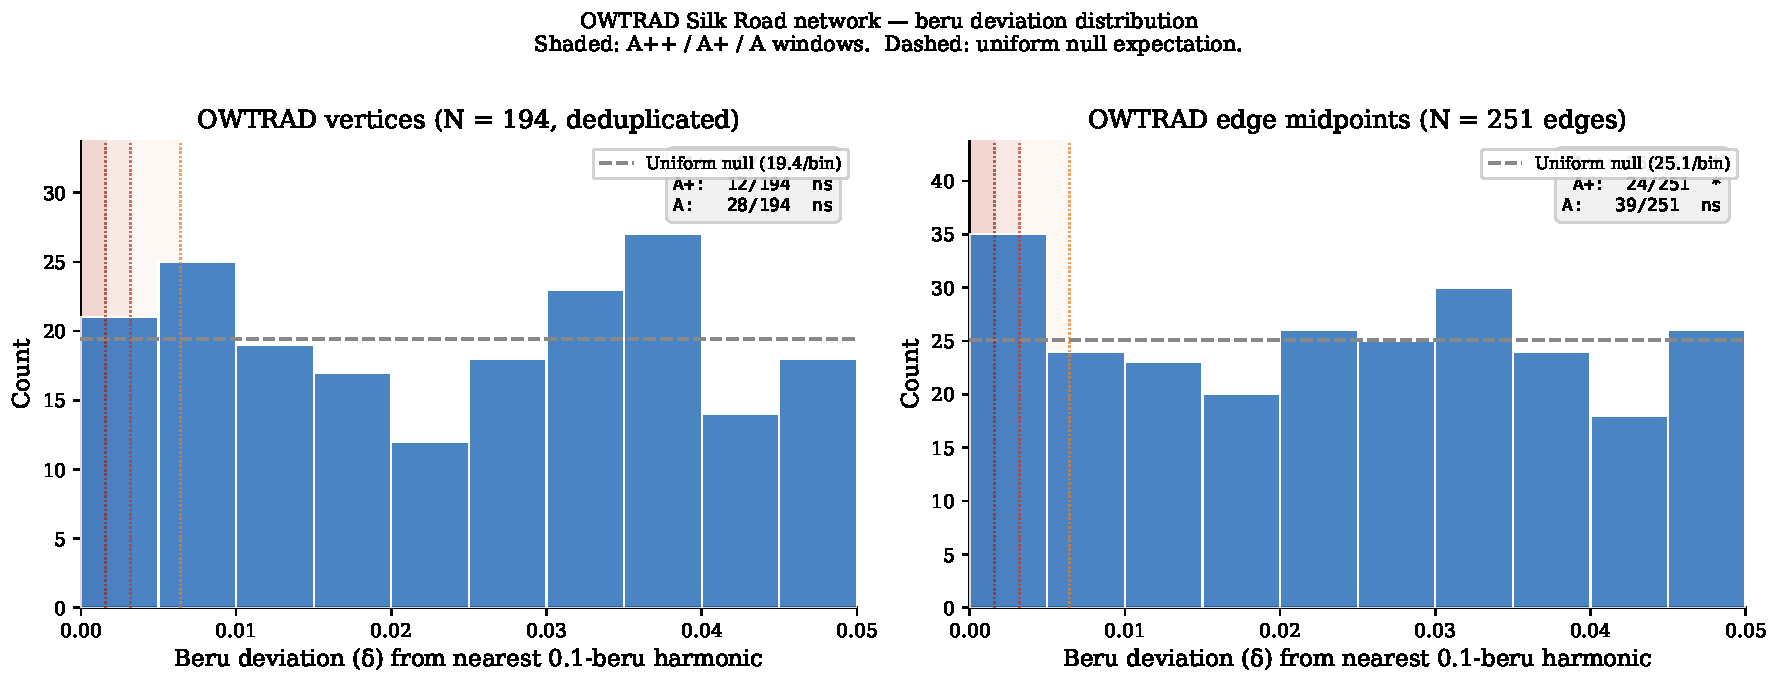
\includegraphics[width=\textwidth]{../figures/fig_owtrad_tiers}
  \caption{OWTRAD Silk Road endpoint tier distributions:
  \NOwtradVertices{} deduplicated endpoints (left) and \NOwtradDegW{} degree-weighted
  route endpoint positions (right).
  The degree-weighted distribution shows A++ enrichment
  ($z = \zOwtradDegWApp$, $p\ \pOwtradDegWApp$~\pOwtradDegWAppSig{});
  the deduplicated endpoint distribution is weaker
  ($z = \zOwtradVertexApp$, $p = \pOwtradVertexApp$~\pOwtradVertexAppSig{}).}
  \label{fig:owtrad_tiers}
\end{figure*}

\begin{figure*}[!t]
  \centering
  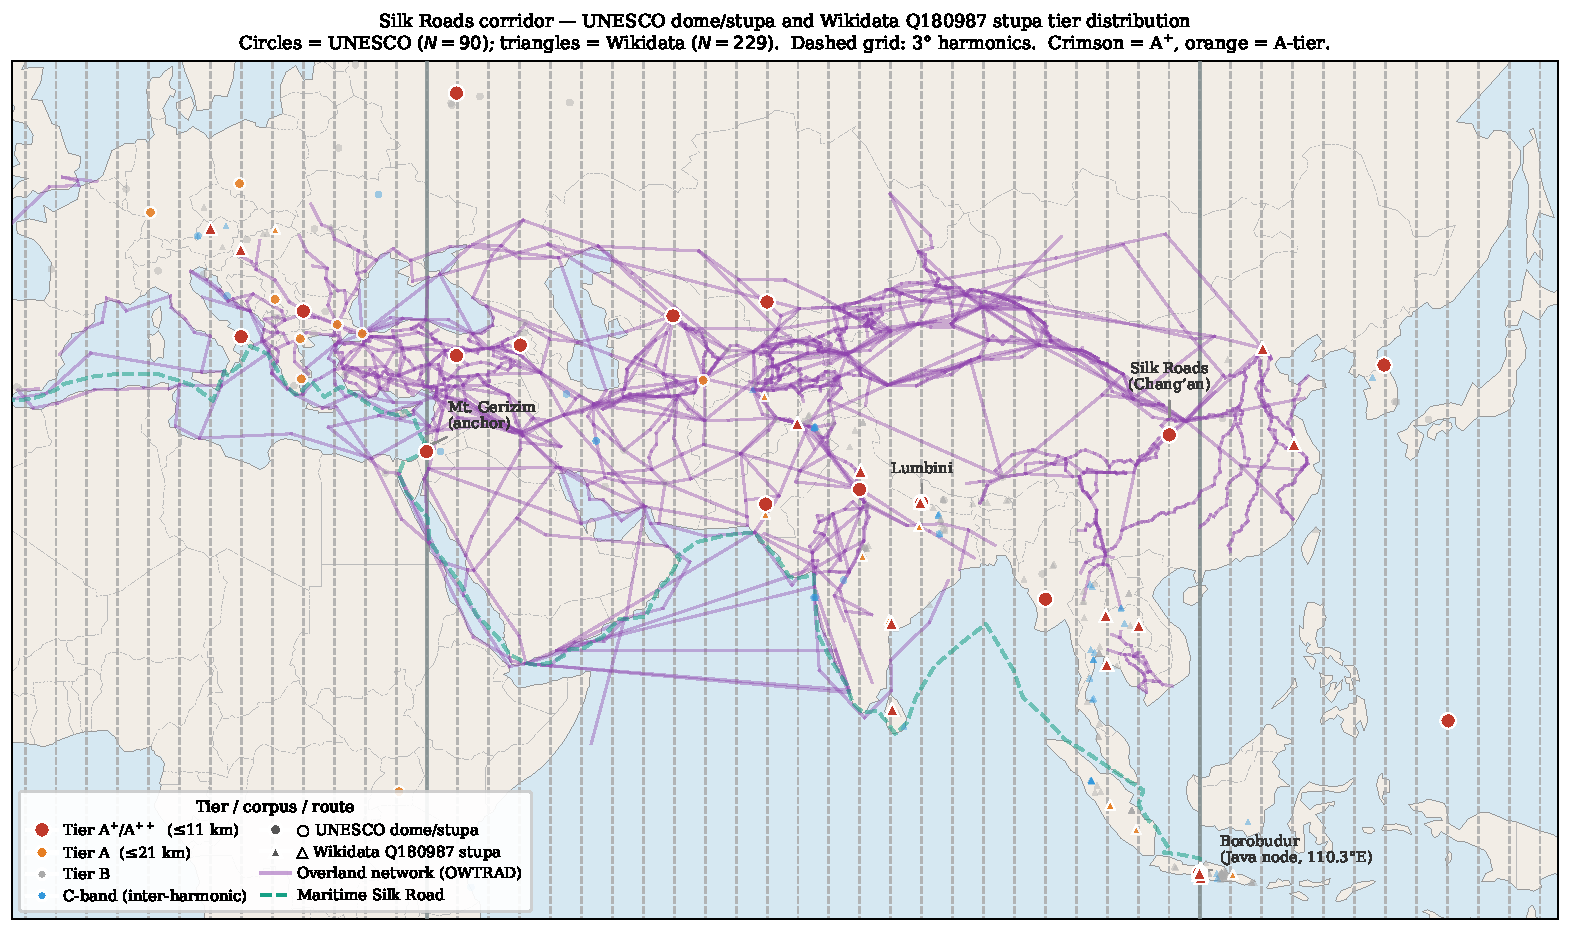
\includegraphics[width=\textwidth]{../figures/fig_geo_trail}
  \caption{Tier distribution of UNESCO domed/stupa and Wikidata Q180987
  stupa sites along the Eurasian corridor.
  Overland route edges from the OWTRAD attested-route database
  \citep{ciolek2004owtrad}.
  Maritime route is a schematic coastal polyline after
  \citet{casson1989periplus}, \citet{sen2014silk}, and \citet{tomber2008rome}.
  An interactive version is provided as supplementary material
  (\texttt{supplementary/interactive\_map/silkroad\_interactive.html}).}
  \label{fig:geo_trail}
\end{figure*}

\section{Conclusion}

This paper reports an exploratory pattern: the UNESCO
Cultural and Mixed corpus shows a consistent template-alignment excess near
the $\sim$35\textdegree{}E corridor under multiple diagnostic checks
(Table~\ref{tab:bonferroni_both}; $p_\mathrm{adj} = \pHolmTestOne$,
$\pHolmTestTwo$, $\pHolmTestThree$), with small effect sizes and
corridor-level rather than point localization. These $p$-values describe
within-frame consistency, not confirmatory evidence.

A multi-scale combined test reduces dependence on any
single tier choice (dome subset $p = \multiscaleDomeCombinedP$~\multiscaleDomeCombinedPSig{};
joint enrichment peaks near \multiscaleJointMaxKm{}~km,
$p = \multiscaleJointMaxP$~\multiscaleJointMaxPSig{}).
The Wikidata stupa corpus and OWTRAD route network show similar enrichment
patterns under the same reference frame (\S\ref{sec:transmission}).

In short, a harmonic-alignment statistic identifies a weak but reproducible
pattern under a specific coordinate representation.
This pattern is not invariant, does not support a periodic generative model,
and is consistent with the interaction between geographic clustering and
the imposed harmonic frame. Its primary contribution is methodological. It
shows how representation choice can induce stable but non-invariant spatial
patterns in culturally clustered datasets.
Independent re-examination on corpora without UNESCO's Eurasian
sampling structure is the appropriate next step.


\appendix

\section{Von Mises Mixture Characterisation of External Corpora}
\label{app:vonmises}

A von~Mises + uniform mixture model
$f(\theta|\kappa) = w \cdot \mathrm{VM}(0,\kappa) + (1-w)\cdot\mathrm{Uniform}(0,2\pi)$
was fitted to the harmonic phase deviations ($\theta \in [0,\pi]$, $\theta=0$
on-harmonic) of two external corpora using maximum likelihood with a
grid of starting values.

OWTRAD Silk Road nodes ($N = \vmNOwtrad{}$):
$\hat{\kappa} = \vmKappaOwtrad{}$, $\hat{w} = \vmMixtureWeightOwtrad{}$,
$\hat{\sigma} = \kappa^{-1/2} = \vmSigmaDegOwtrad{}^\circ$.

Wikidata Q180987 stupas ($N = \vmNStupa{}$):
$\hat{\kappa} = \vmKappaStupa{}$, $\hat{w} = \vmMixtureWeightStupa{}$,
$\hat{\sigma} = \vmSigmaDegStupa{}^\circ$.

$N$-weighted pooled $\hat{\sigma} = \vmSigmaDegPooled{}^\circ$;
$\kappa$ ratio = \vmKappaRatio{} across corpora.

These values characterize external-corpus clustering and are not used to
derive tier boundaries; agreement with tier widths is descriptive context.

\section{Tier-Threshold Sensitivity Audit}
\label{app:tier_sensitivity}

A log-scale null-rate sweep across \logSweepNtaus{} thresholds supports
the interpretation that enrichment is not an artifact of the specific tier width:
\logSweepNsig{} of \logSweepNtaus{} thresholds reach $p < 0.05$ for the
dome subset; dome OR ranges \logSweepMinEnrichCanon{}$\times$--\logSweepMaxEnrichCanon{}$\times$
across the three canonical tiers (A, A+, A++).
Within $\pm$1 log-decade of the A+ threshold,
\logSweepAregionNsig{} of \logSweepAregionNtaus{} thresholds are significant.
Full results in \texttt{supplementary/audit/tier\_sensitivity\_audit.txt}.


%------------------------------------------------------------------------------
\section{Keyword Audit Summary}
\label{sec:kwdaudit}

Full site-by-site audit files are indexed in Supplementary~S1
(\path{supplementary/Supplementary_S1.md}; \citealt{tenenbaum2026audit});
regenerate all with \texttt{bash} \path{tools/update_all_audits.sh}.

\subsection{Dome/Spherical Monument Filter (Tests~1, 5, 5x, 6x)}
\label{sec:kwdaudit_dome}

\NcircKeywords{} morphological keywords from four roots
(\textit{stupa/stupas}, \textit{tholos}, \textit{dome/domed/domes},
\textit{spherical}) are matched as whole words against each site's
name, XML description, and extended OUV text. All \NcircTotal{} matching
sites are included in the Test~1 dome mixture and Test~5 tier-enrichment
analyses without context gating.

For Test~5x, ambiguous keywords (\textit{dome, domed, domes, spherical})
are subject to a two-gate context check: Gate~1 (\NdomeGateNeg{} negative
patterns) rejects non-architectural uses; Gate~2 (\NdomeGatePos{} positive
patterns) requires architectural confirmation. Unambiguous keywords
(\textit{stupa/stupas}, \textit{tholos}) are accepted without validation.
The seven
rejected sites are: Hiroshima Peace Memorial, Richtersveld, Gyeongju,
Vi\~{n}ales Valley, Rock Islands Southern Lagoon, Uluru-Kata Tju\d{t}a,
and Diqu\'{i}s Stone Spheres.

\hyperref[sec:resultsevolution_inline]{Test~6} adds earthen mound-stage
keywords (\textit{tumulus, tumuli, barrow, barrows, kofun} unambiguous;
\textit{mound} context-validated) to trace the hemispherical tradition
from burial mound through stupa to architectural dome. Test~6x applies
the same architectural context gates to the extended population.
Statistics for all four variants are reported in
\hyperref[sec:resultscircular]{\S\ref*{sec:resultscircular}} and
\hyperref[sec:resultsevolution_inline]{\S\ref*{sec:resultsevolution_inline}}.

\subsection{Founding-Origin Classifier (Post-Hoc)}
\label{sec:kwdaudit_founding}

\textbf{Results.} The classifier finds \foundKwApRate\% of A+ sites
carry a founding keyword versus \foundKwBaseRate\% in the full corpus
(Fisher OR~$= \foundKwFisherOR$, $p = \pFoundKwFisher$~\pFoundKwFisherSig{}).
The A++ sub-population (\NfoundKwTotalApp{} sites) shows a stronger
signal: \foundKwAppRate\% carry a founding keyword
(OR~$= \foundKwAppFisherOR$, $p = \pFoundKwAppFisher$~\pFoundKwAppFisherSig{}),
consistent with the most precisely aligned sites being disproportionately
historically foundational monuments.

The classifier assigns sites to five founding-related categories; full
keyword definitions and the site-by-site listing are in the supplementary
archive \citep{tenenbaum2026audit}.



%------------------------------------------------------------------------------

\begin{thebibliography}{99}
%------------------------------------------------------------------------------

\bibitem[Aveni(2001)]{aveni2001skywatchers}
Aveni, A.~F. (2001).
\textit{Skywatchers: A Revised and Updated Version of Skywatchers of
Ancient Mexico}.
University of Texas Press.

\bibitem[Aveni(2003)]{aveni2003archaeoastronomy}
Aveni, A.~F. (2003).
Archaeoastronomy in the ancient Americas.
\textit{Journal of Archaeological Research}, 11(2), 149--191.

\bibitem[Casson(1989)]{casson1989periplus}
Casson, L. (1989).
\textit{The Periplus Maris Erythraei: Text with Introduction, Translation,
and Commentary}.
Princeton University Press.

\bibitem[Ciolek(2004)]{ciolek2004owtrad}
Ciolek, T.~M. (2004).
\textit{Old World Trade Routes (OWTRAD) Project}.
Asia Pacific Research Online, Canberra.
\url{http://www.ciolek.com/OWTRAD/DATA/tmcOWTRAD.html}

\bibitem[Benjamini \& Hochberg(1995)]{benjamini1995controlling}
Benjamini, Y. \& Hochberg, Y. (1995).
Controlling the false discovery rate: a practical and powerful approach
to multiple testing.
\textit{Journal of the Royal Statistical Society, Series B}, 57(1), 289--300.

\bibitem[Crown(1989)]{crown1989}
Crown, A.~D. (1989).
\textit{The Samaritans}.
J.~C.~B. Mohr (Paul Siebeck).

\bibitem[Freeman(1976)]{freeman1976}
Freeman, P.~R. (1976).
A Bayesian analysis of the megalithic yard.
\textit{Journal of the Royal Statistical Society, Series A}, 139(1), 20--35.

\bibitem[Good(2005)]{good2005permutation}
Good, P.~I. (2005).
\textit{Permutation, Parametric, and Bootstrap Tests of Hypotheses}
(3rd ed.).
Springer.

\bibitem[Holm(1979)]{holm1979simple}
Holm, S. (1979).
A simple sequentially rejective multiple test procedure.
\textit{Scandinavian Journal of Statistics}, 6(2), 65--70.

\bibitem[Hansen(2012)]{hansen2012silkroad}
Hansen, V. (2012).
\textit{The Silk Road: A New History}.
Oxford University Press.

\bibitem[Harvey(1987)]{harvey1987mappamundi}
Harvey, P.~D.~A. (1987).
Medieval maps of the world.
In J.~B.~Harley \& D.~Woodward (Eds.),
\textit{The History of Cartography, Volume~1:
Cartography in Prehistoric, Ancient, and Medieval Europe
and the Mediterranean} (pp.~283--370).
University of Chicago Press.

\bibitem[Burton(1893)]{burton1893pilgrimage}
Burton, R.~F. (1893).
\textit{Personal Narrative of a Pilgrimage to Al-Madinah \& Meccah},
vol.~2 (Memorial Edition), p.~63, n.~2.
Tylston and Edwards.

\bibitem[Hunger \& Steele(2019)]{hunger2019mul}
Hunger, H. \& Steele, J. (2019).
\textit{The Babylonian Astronomical Compendium MUL.APIN}.
Routledge.

\bibitem[Thureau-Dangin(1921)]{thureau1921}
Thureau-Dangin, F. (1921).
\textit{Num\'eration et m\'etrologie sum\'eriennes}.
Revue d'Assyriologie et d'arch\'eologie orientale, 18, 123--142.

\bibitem[Kendall(1974)]{kendall1974}
Kendall, D.~G. (1974).
Hunting quanta.
\textit{Philosophical Transactions of the Royal Society A}, 276(1257), 231--266.

\bibitem[MacDonald(1964)]{macdonald1964}
MacDonald, J. (1964).
\textit{The Theology of the Samaritans}.
SCM Press.

\bibitem[Mardia \& Jupp(2000)]{mardia2000directional}
Mardia, K.~V. \& Jupp, P.~E. (2000).
\textit{Directional Statistics}.
Wiley.

\bibitem[Magli(2013)]{magli2013}
Magli, G. (2013).
\textit{Architecture, Astronomy and Sacred Landscape in Ancient Egypt}.
Cambridge University Press.

\bibitem[Magli(2016)]{magli2016}
Magli, G. (2016).
\textit{Archaeoastronomy: Introduction to the Science of Stars and Stones}.
Springer.

\bibitem[Miksic(1990)]{miksic1990borobudur}
Miksic, J.~N. (1990).
\textit{Borobudur: Golden Tales of the Buddhas}.
Periplus Editions.

\bibitem[Neugebauer(1975)]{neugebauer1975history}
Neugebauer, O. (1975).
\textit{A History of Ancient Mathematical Astronomy}, 3~vols.
Springer.

\bibitem[Powell(1987)]{powell1987metrological}
Powell, M.~A. (1987).
Masse und Gewichte.
In D. O. Edzard (Ed.),
\textit{Reallexikon der Assyriologie und Vorderasiatischen Arch\"aologie},
vol.~7, pp.~457--517. Walter de Gruyter.

\bibitem[Purvis(1968)]{purvis1968}
Purvis, J.~D. (1968).
\textit{The Samaritan Pentateuch and the Origin of the Samaritan Sect}.
Harvard University Press.

\bibitem[Robson(2008)]{robson2008mathematics}
Robson, E. (2008).
\textit{Mathematics in Ancient Iraq: A Social History}.
Princeton University Press.

\bibitem[Ruggles(1999)]{ruggles1999astronomy}
Ruggles, C.~L.~N. (1999).
\textit{Astronomy in Prehistoric Britain and Ireland}.
Yale University Press.

\bibitem[Ruggles \& Cotte(2010)]{ruggles2010icomos}
Ruggles, C.~L.~N. \& Cotte, M. (Eds.) (2010).
\textit{Heritage Sites of Astronomy and Archaeoastronomy in the Context
of the UNESCO World Heritage Convention: A Thematic Study}.
ICOMOS \& International Astronomical Union.

\bibitem[Ruggles(2015)]{ruggles2015handbook}
Ruggles, C.~L.~N. (Ed.) (2015).
\textit{Handbook of Archaeoastronomy and Ethnoastronomy}.
Springer.

\bibitem[Sen(2014)]{sen2014silk}
Sen, T. (2014).
The spread of Buddhism.
In B.~Z.~Kedar \& M.~E.~Wiesner-Hanks (Eds.),
\textit{The Cambridge World History, Vol.~5: Expanding Webs of Exchange
and Conflict, 500 CE--1500 CE} (pp.~447--479).
Cambridge University Press.

\bibitem[Silva(2020)]{silva2020statistical}
Silva, F. (2020).
A probabilistic framework and significance test for the analysis
of structural orientations in skyscape archaeology.
\textit{Journal of Archaeological Science}, 118, 105138.

\bibitem[Tenenbaum(2026)]{tenenbaum2026audit}
Tenenbaum, S. (2026).
\textit{Longitude Quantization in the UNESCO World Heritage Corpus: Domes, Stupas, and 3\textdegree{} Harmonics: Code and Data} (v1.6.0).
Zenodo. \url{https://doi.org/10.5281/zenodo.19938283}

\bibitem[Tomber(2008)]{tomber2008rome}
Tomber, R. (2008).
\textit{Indo-Roman Trade: From Pots to Pepper}.
Duckworth.

\bibitem[Thom(1964)]{thom1964}
Thom, A. (1964).
The larger units of length of megalithic man.
\textit{Journal of the Royal Statistical Society, Series~A}, 127(4), 527--533.

\bibitem[Thom(1967)]{thom1967}
Thom, A. (1967).
\textit{Megalithic Sites in Britain}.
Oxford University Press.

\bibitem[Thom(1971)]{thom1971}
Thom, A. (1971).
\textit{Megalithic Lunar Observatories}.
Oxford University Press.

\bibitem[UNESCO World Heritage Centre(2024)]{unescowhc2024xml}
{UNESCO World Heritage Centre}. (2024).
\textit{World Heritage List} [XML dataset].
Retrieved from \url{https://whc.unesco.org/en/list/xml/}.

\bibitem[Watson \& Horowitz(2011)]{watson2011writing}
Watson, R.~T. \& Horowitz, W. (2011).
\textit{Writing Science Before the Greeks: A Naturalistic Analysis of the
Babylonian Astronomical Treatise MUL.APIN}.
Brill.

\bibitem[Williamson \& Bellamy(1983)]{williamson1983leylines}
Williamson, T. \& Bellamy, L. (1983).
\textit{Ley Lines in Question}.
World's Work.

\end{thebibliography}


\section*{Data Availability Statement}
\label{sec:data_code}
All data and code are openly available; a permanent snapshot (v1.6.0) is
deposited at Zenodo (\citealt{tenenbaum2026audit};
\url{https://doi.org/10.5281/zenodo.19938283}); UNESCO XML: \citealt{unescowhc2024xml}.
Scripts, audit files, and maps are indexed in
Supplementary~S1 (\texttt{supplementary/Supplementary\_S1.md}), with each
file's role, macros produced, and paper section noted.
Full reproduction: \texttt{reproduce\_all\_macros.sh},
\texttt{update\_all\_audits.sh}, \texttt{generate\_figures.py}.

\section*{Acknowledgements}
The UNESCO World Heritage Centre maintains the publicly accessible XML
dataset on which this study depends. This research was conducted independently and without external institutional affiliation.

\section*{Conflict of Interest}
The author declares no conflict of interest.

\section*{Software and AI Disclosure}
All statistical analyses were performed in Python~3 using NumPy, SciPy, and pandas.
Large-language-model tools were used during preparation of this manuscript:
Claude (Anthropic) assisted with prose drafting and editing;
GitHub Copilot (Microsoft) assisted with code autocompletion.
These tools were used solely as writing and coding aids.
All scientific hypotheses, analytical choices, keyword-list decisions,
interpretation of results, and conclusions are solely the responsibility of the author.
No AI tool was used to generate, fabricate, or substitute for primary data or statistical analysis.


\end{document}
